\documentclass[a4paper,12pt]{report}

% Pacotes ----------------------------------------------------------------------
% Margens ----------------------------------------------------------------------
\usepackage[top=3cm,left=3cm,right=2cm,bottom=2cm]{geometry}

% Pacotes Principais -----------------------------------------------------------
\usepackage[portuges,brazil]{babel}
\usepackage[utf8]{inputenc}
\usepackage[T1]{fontenc} 
\usepackage{ae}
\usepackage{indentfirst} % Indenta os primeiros parágrafos

% Fórmulas
\usepackage{icomma}
\usepackage{cancel}

% Formatação
\usepackage{url}

% Figuras e Imagens ------------------------------------------------------------
\usepackage{graphicx}
% Figuras lado a lado
\usepackage{epsfig}
\usepackage{subfigure}
\usepackage{color}

% Utilizar H para inserir as imagens REALMENTE onde eu desejo
\usepackage{float}

% Fontes -----------------------------------------------------------------------
\usepackage[T1]{fontenc}
\usepackage{pslatex}

% Simbolos ---------------------------------------------------------------------
\usepackage{textcomp}
\usepackage{amsmath}
\usepackage{mathrsfs}

% Tabelas ----------------------------------------------------------------------
%\usepackage{multicol}
\usepackage{multirow}

% Codigos ----------------------------------------------------------------------
% Comentários em bloco
\usepackage{verbatim}
\usepackage{listings}

% Biliografia ------------------------------------------------------------------
\usepackage{harvard}
\harvardparenthesis{square}
\harvardyearparenthesis{round}
\renewcommand{\harvardand}{e}


% Comandos ---------------------------------------------------------------------
\setlength{\parindent}{1cm}
\newcommand{\mbf}[1]{\mathbf{#1}}
\let\D\displaystyle


% In�cio do documento ----------------------------------------------------------
\begin{document}

%\tableofcontents
\begin{titlepage}
\begin{center}

\begin{table}[h]
\centering
\setlength{\arrayrulewidth}{3.5\arrayrulewidth}
    \begin{tabular}{cc}
    \hline\\
    \multirow{5}{*}{
\includegraphics[height=3cm]{imgs/ufrn}}&\\
    & \textsc{Universidade Federal do Rio Grande do Norte}\\
    & \textsc{Programa de P�s-Gradua��o em}\\
    & \textsc{Engenharia El�trica e de Computa��o}\\
    & \textsc{[EEC 2101] Controle Avan�ado}\\
    &\\
    &\\
    \hline
    \end{tabular}
\end{table}


\vfill

\LARGE
\textbf{1\textordfeminine\ Lista de Exerc�cios}

\vfill

\normalsize
\textbf{Anna Giselle C�mara Dantas Ribeiro}\\
\textbf{Cristiano Gurgel de Castro}\\
\textbf{Diogo Leite Rebou�as}\\
\textbf{Thiago Medeiros Barros}

\vfill
\textbf{Natal -- RN\\
        2010.1 }

\end{center}
\end{titlepage}

\section*{Questão 1}
% Enunciado
\noindent {\it Um sistema com realimentação unitária tem a seguinte função de
transferência de malha aberta:}

\begin{equation}\nonumber
G(s) = \frac{9}{s(s+p)}
\end{equation}

\noindent {\it em que $p$ é normalmente igual a 3. Determine a sensibilidade da
função de transferência de malha fechada $T(s)$ em relação ao parâmetro $p$ e
plote os diagramas de Bode (módulo e fase) para $p$ variando entre 1 e 5.
Analise os resultados.}

\vspace{0.5cm}

\noindent{\bf Resolução:}

\vspace{0.25cm}

Antes de realizar a análise da sensibilidade em malha fechada, deve-se verificar
a estabilidade relativa do sistema em malha aberta quanto à variação do
parâmetro $p$. 

Sabe-se que essa estabilidade relativa pode ser observada a partir de duas
medidas dos diagramas de Bode, denominadas {\it margem de ganho} e {\it margem
de fase}. Para \citeasnoun{dorf:2009}, a {\it margem de ganho} é definida como
um acréscimo no ganho do sistema quando a fase é igual a -180\textdegree,
resultando em um sistema marginalmente estável, enquanto que a {\it margem de
fase} é definida como a quantidade de deslocamento de fase com magnitude
unitária que resultará em um sistema marginalmente estável.

Assim sendo, ao se observar a Fig. \ref{fig:bode_ma}, verifica-se que essas duas
medidas variam conforme Tab. \ref{tab:margem_ganho_fase_ma} para o sistema em
malha aberta\footnote{Apesar dos diagramas de Bode exibidos ao longo de toda a
resolução estarem sendo referenciados às equações no domínio de {\it Laplace}
com a variável complexa $s$, obter equações no domínio da frequência resume-se a
substituir a variável $s$ por $j\omega$.}.

\begin{figure}[htb]
\centering
    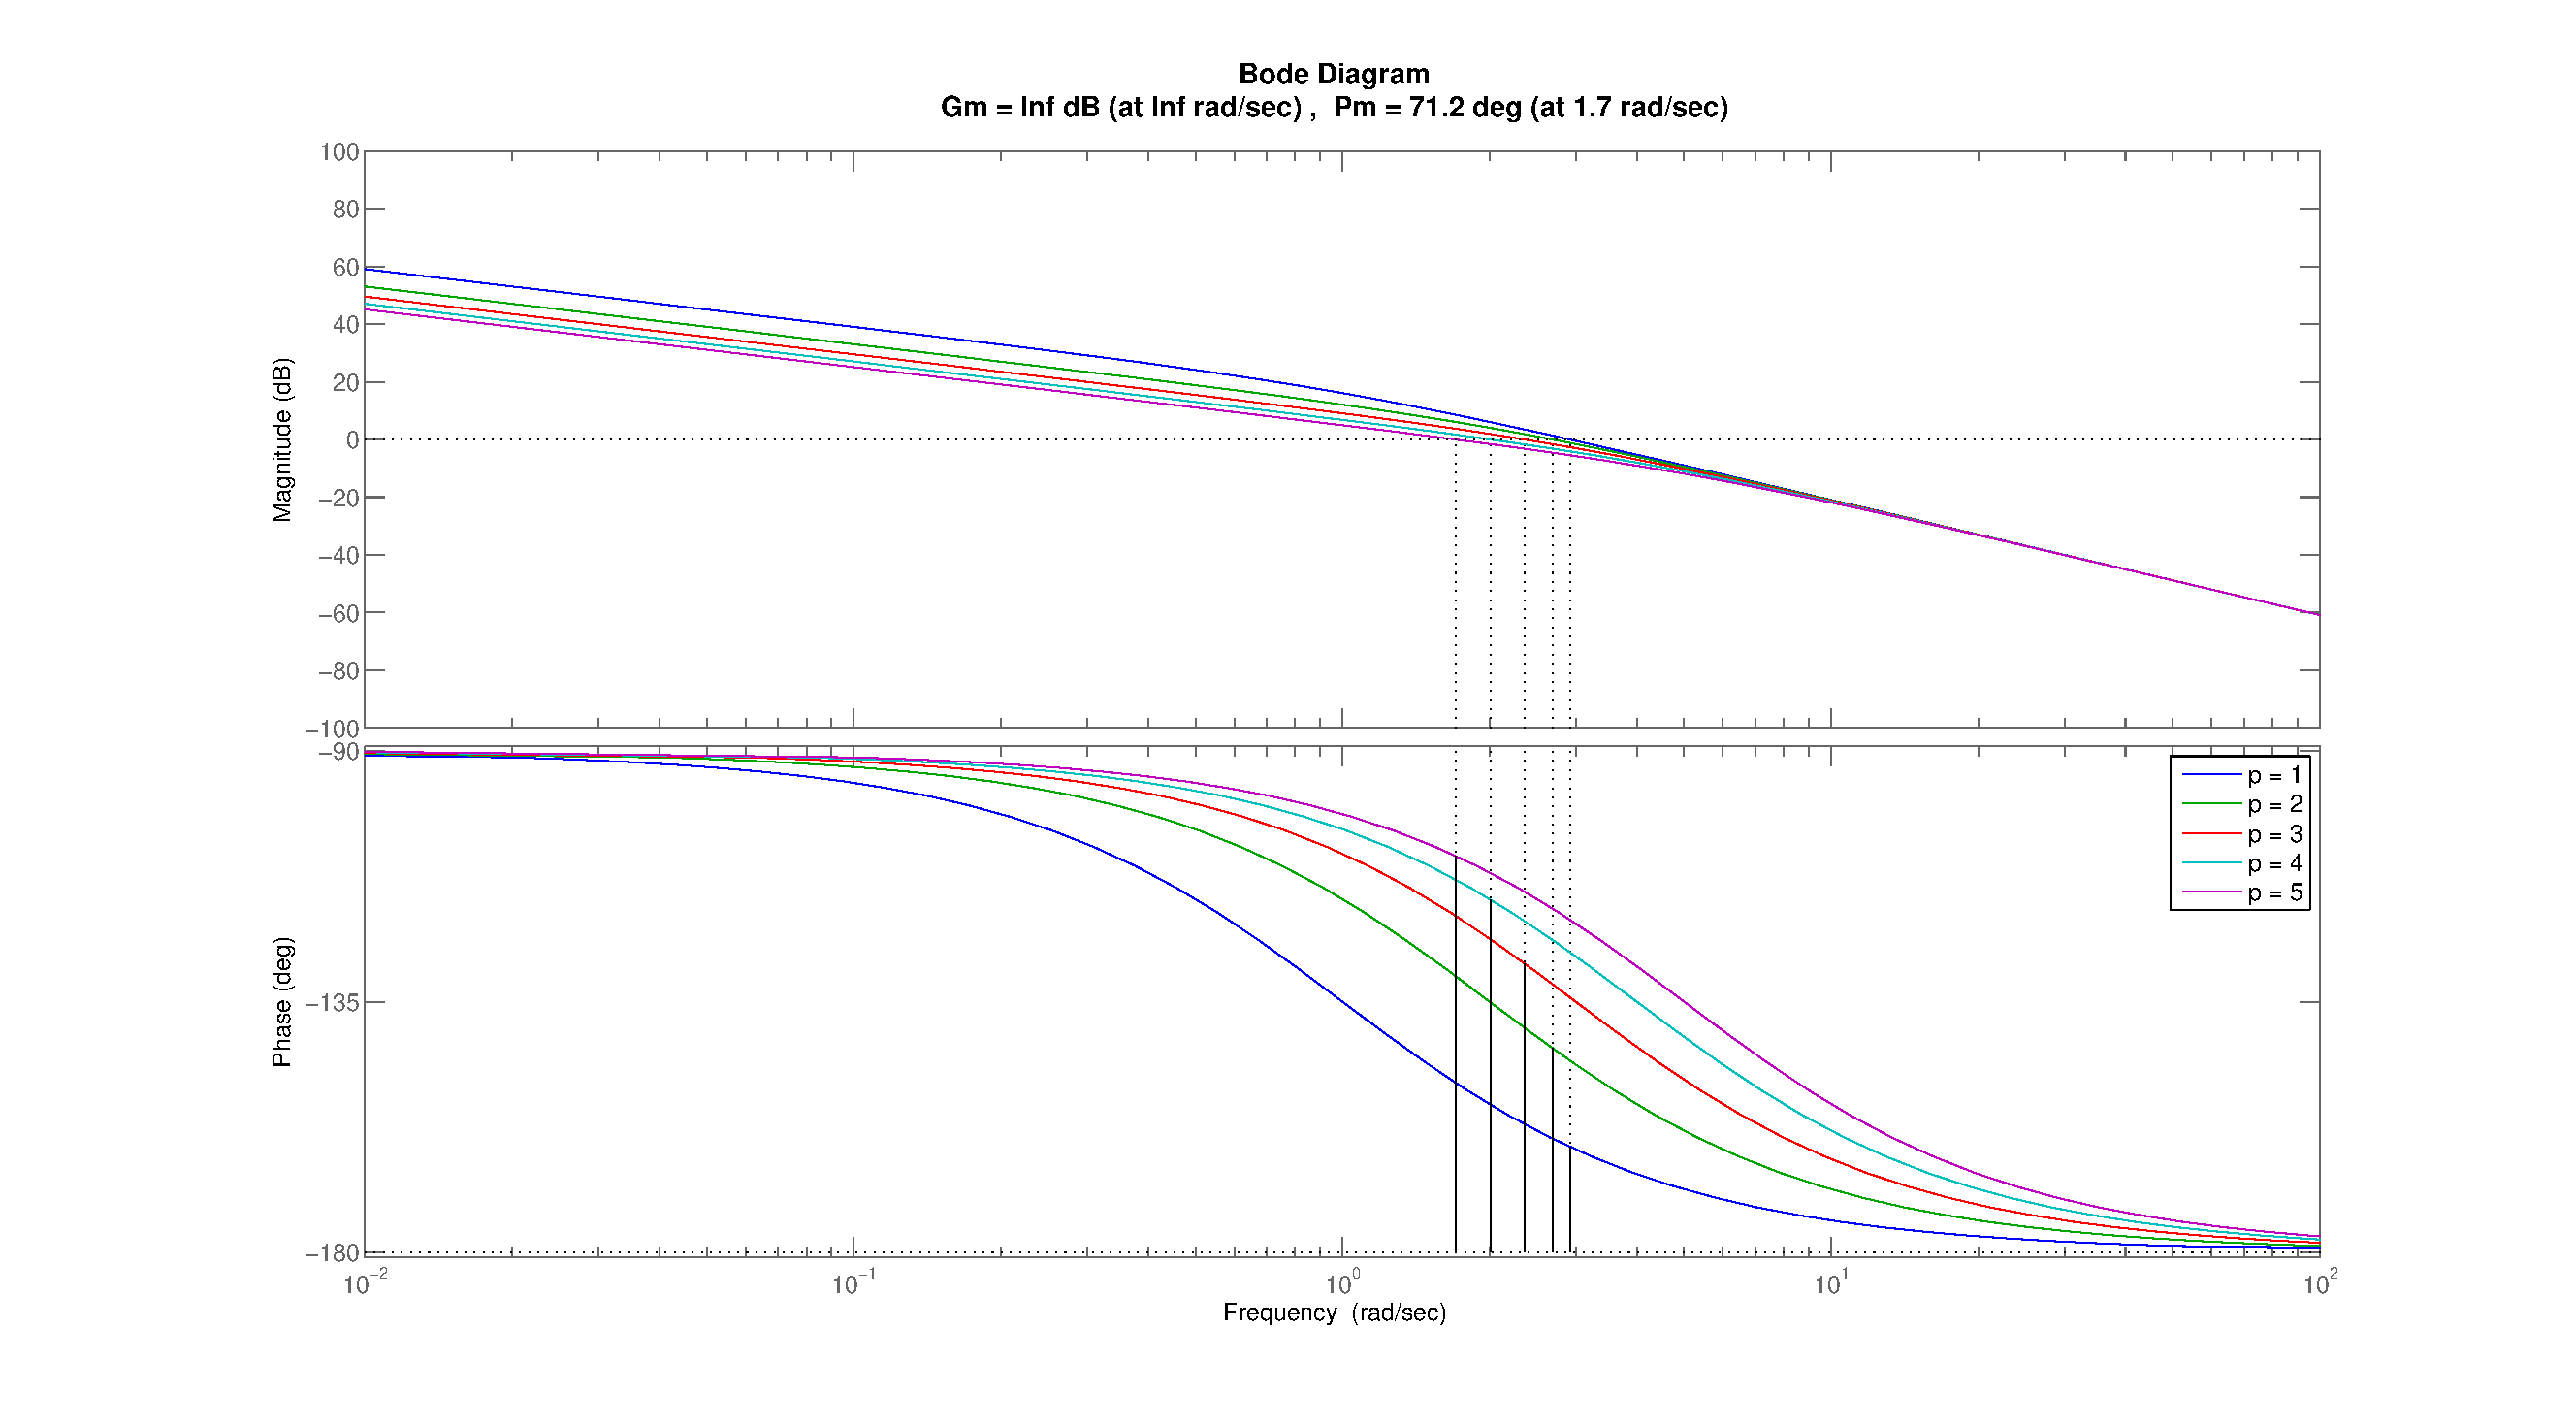
\includegraphics[width=0.95\textwidth]{imgs/questao1/bode_ma}
    \caption{Diagrama de bode para o sistema em malha aberta.}
    \label{fig:bode_ma}
\end{figure}

\begin{table}
\centering
    \caption{Margem de ganho e margem de fase para o sistema em malha aberta.}
    \label{tab:margem_ganho_fase_ma}
    \vspace{0.25cm}
\begin{tabular}{|c|c|c|c|c|}
\hline
$p$ & Margem de Ganho (MG) & $\omega_\text{MG}$ & 
Margem de Fase (MF) & $\omega_\text{MF}$\\
\hline
\hline
1 & $\infty$ & $\infty$ & 18.9175 & 2.9179\\
\hline
2 & $\infty$ & $\infty$ & 36.6620 & 2.6869\\
\hline
3 & $\infty$ & $\infty$ & 51.8273 & 2.3585\\
\hline
4 & $\infty$ & $\infty$ & 63.3162 & 2.0104\\
\hline
5 & $\infty$ & $\infty$ & 71.1830 & 1.7038\\
\hline
\end{tabular}
\end{table}

Sabendo que o sistema será estável quando a margem de ganho e a margem de fase
forem positivas, percebe-se que para os valores de $p = 1\text{,}\ 2\text{,}\ 
\ldots\text{,}\ 5$, o sistema é estável.

Dessa maneira, deseja-se agora realizar a análise em malha fechada. Para isso, a
função de transferência de malha fechada pode ser obtida a partir da Eq.
\ref{eq:G_MF}:

\begin{equation}\label{eq:G_MF}
G_{MF}(s) = \frac{G(s)}{1+G(s)H(s)}
\end{equation}

\noindent na qual $G(s)$ é função de transferência de malha aberta e $H(s)$ a
função de transferência do bloco da realimentação, conforme Fig.
\ref{fig:diag_bloco}. Assim sendo, a função de transferência de malha fechada
para o sistema do enunciado com realimentação unitária é dada pela Eq.
\ref{eq:G_MF_q1}:

\begin{figure}[htb]
\centering
    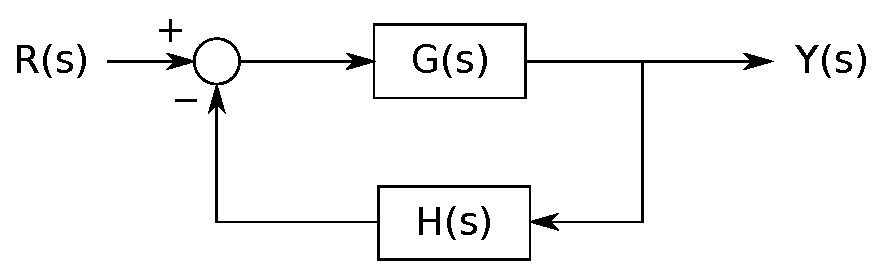
\includegraphics[width=0.55\textwidth]{imgs/questao1/diag_bloco}
    \caption{Diagrama de blocos de um sistema realimentado.}
    \label{fig:diag_bloco}
\end{figure}

\begin{eqnarray}
G_{MF}(s) & = & \frac{G(s)}{1+G(s)H(s)}\nonumber\\
          & = & \frac{G(s)}{1+G(s)}\nonumber\\
          & = & \frac{\D\frac{9}{s(s+p)}}{1+\D\frac{9}{s(s+p)}}\nonumber\\
          & = & \frac{\D\frac{9}{s(s+p)}}{\D\frac{s(s+p)+9}{s(s+p)}}\nonumber\\
          & = & \frac{9}{s(s+p)+9}\nonumber\\
          & = & \frac{9}{s^2 + ps + 9}\label{eq:G_MF_q1}
\end{eqnarray}

Observando a Fig. \ref{fig:bode_mf}, percebe-se que o sistema possuirá um
comportamento oscilatório característico das curvas com picos no diagrama de
Bode. Tal comportamento é comprovado a partir da resposta ao degrau unitário,
conforme Fig. \ref{fig:resp_deg_mf}.

\begin{figure}[htb]
\centering
    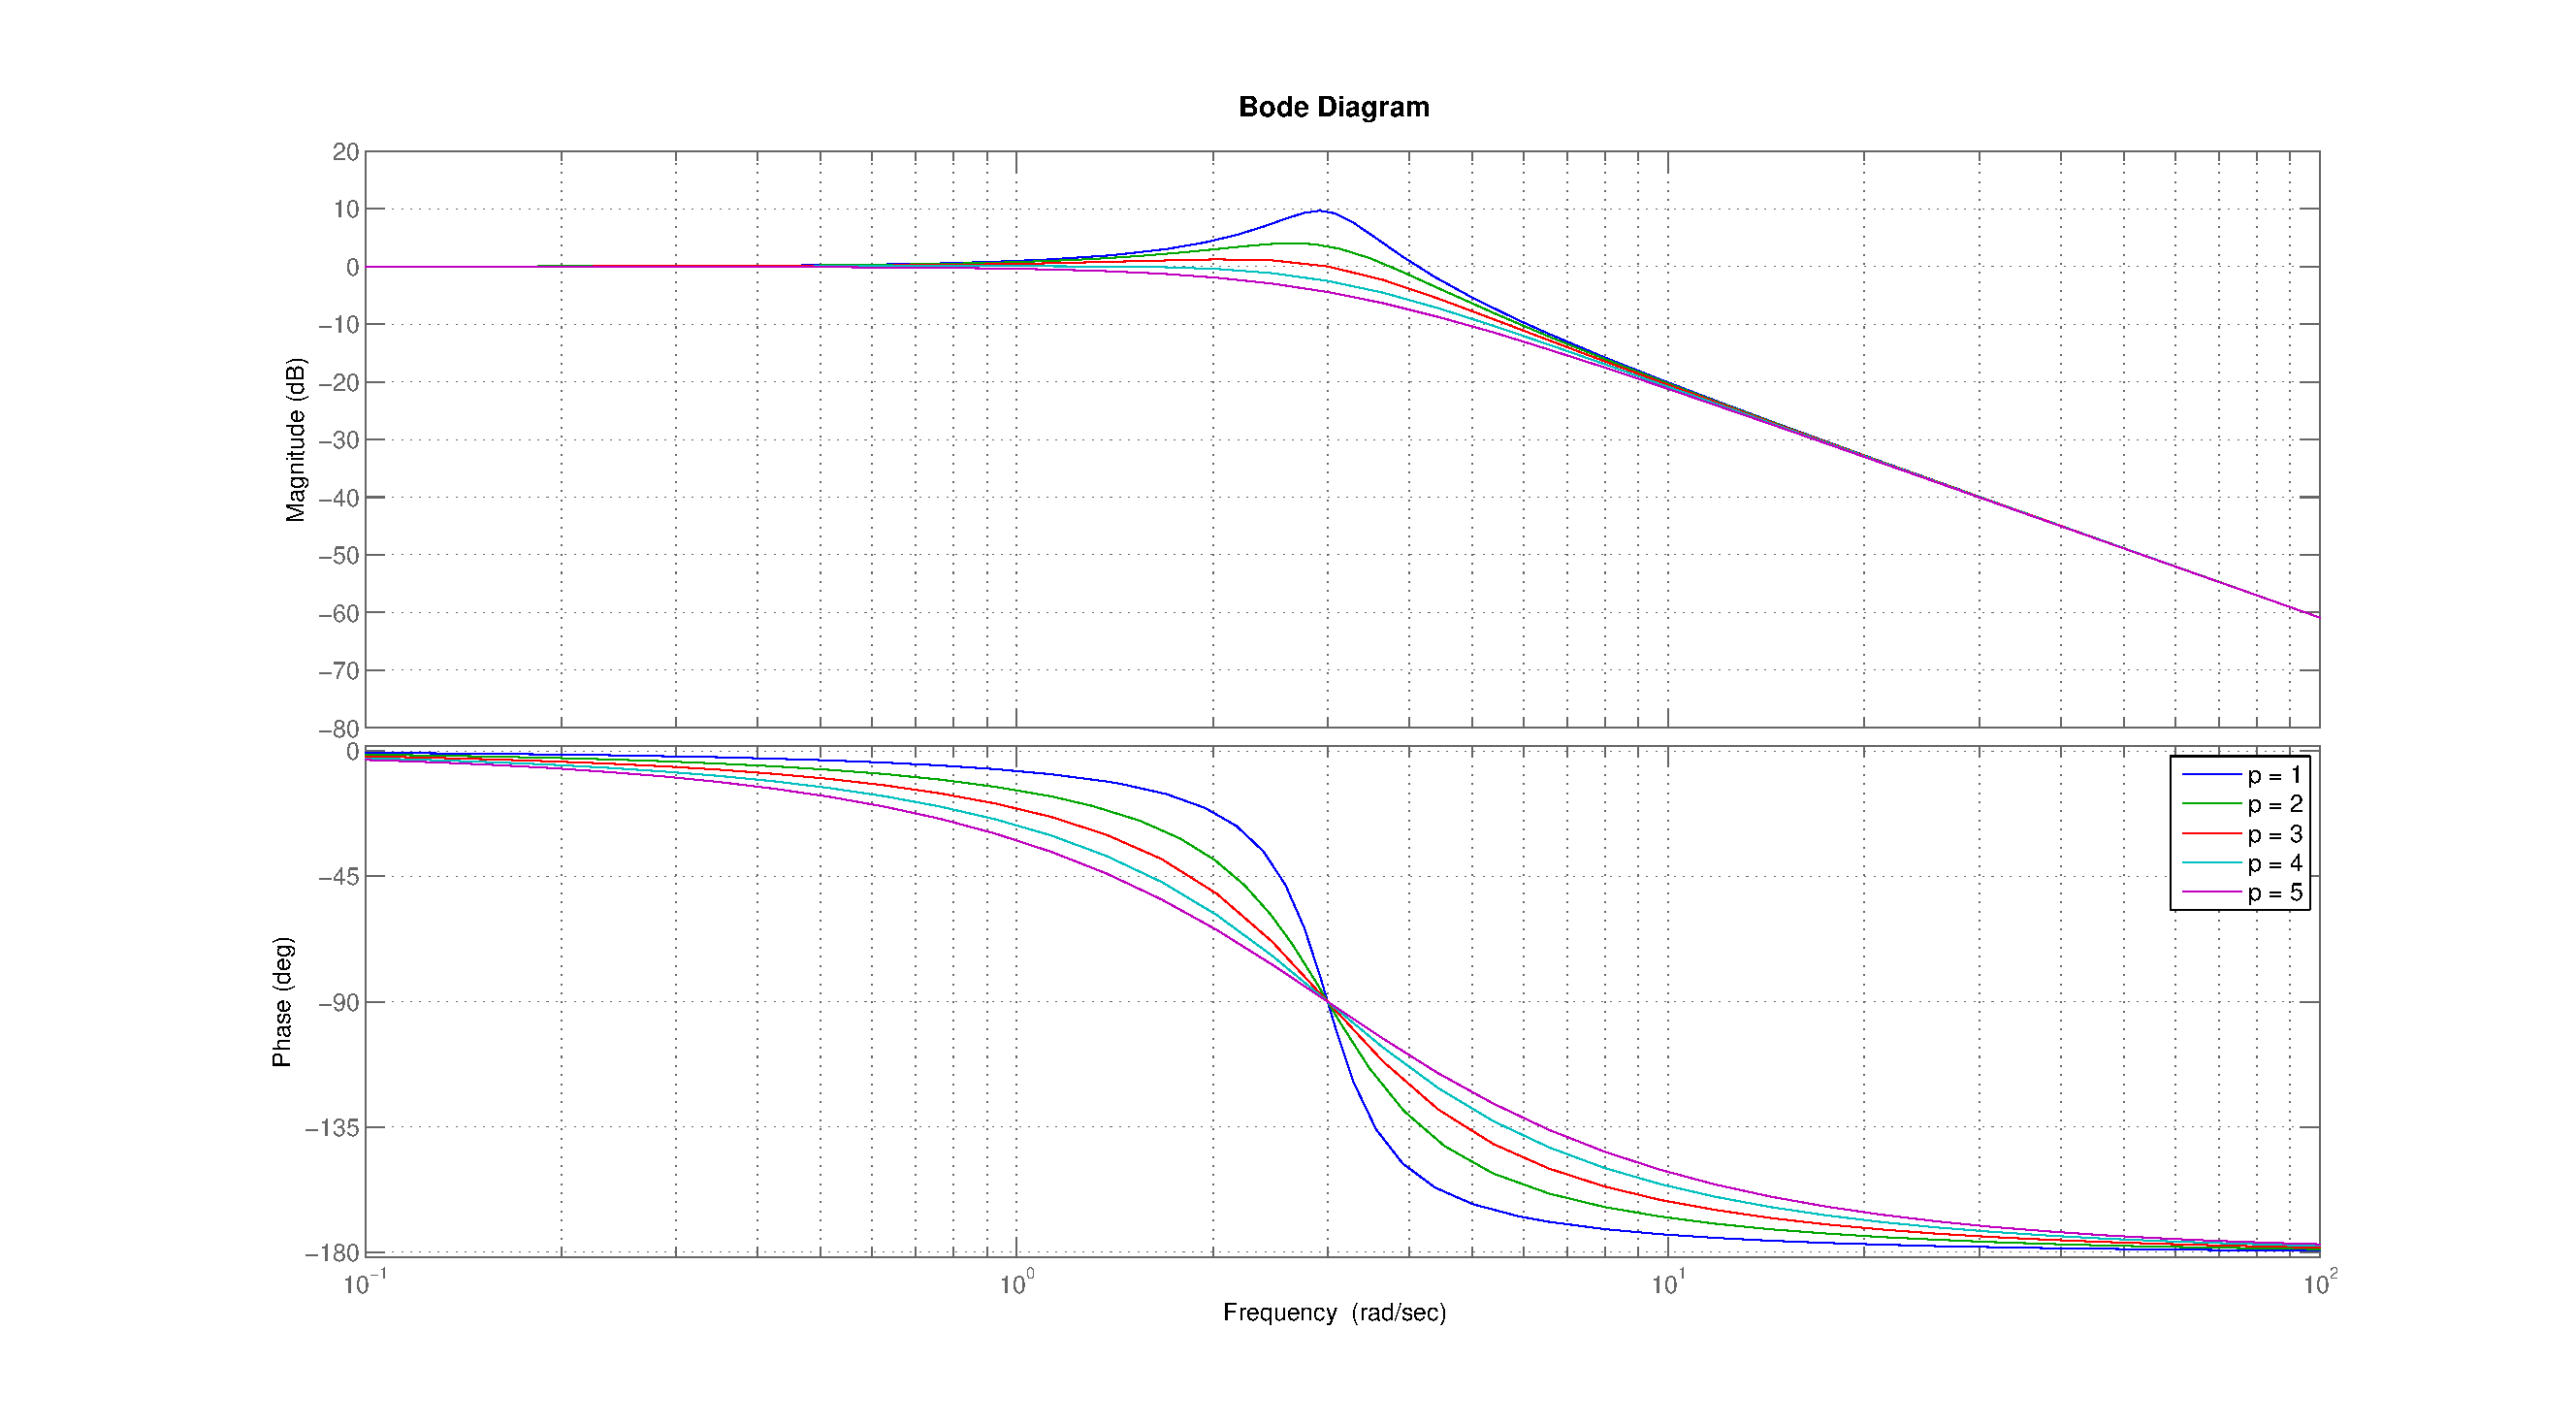
\includegraphics[width=0.95\textwidth]{imgs/questao1/bode_mf}
    \caption{Diagrama de bode para o sistema em malha fechada.}
    \label{fig:bode_mf}
\end{figure}

\begin{figure}[htb]
\centering
    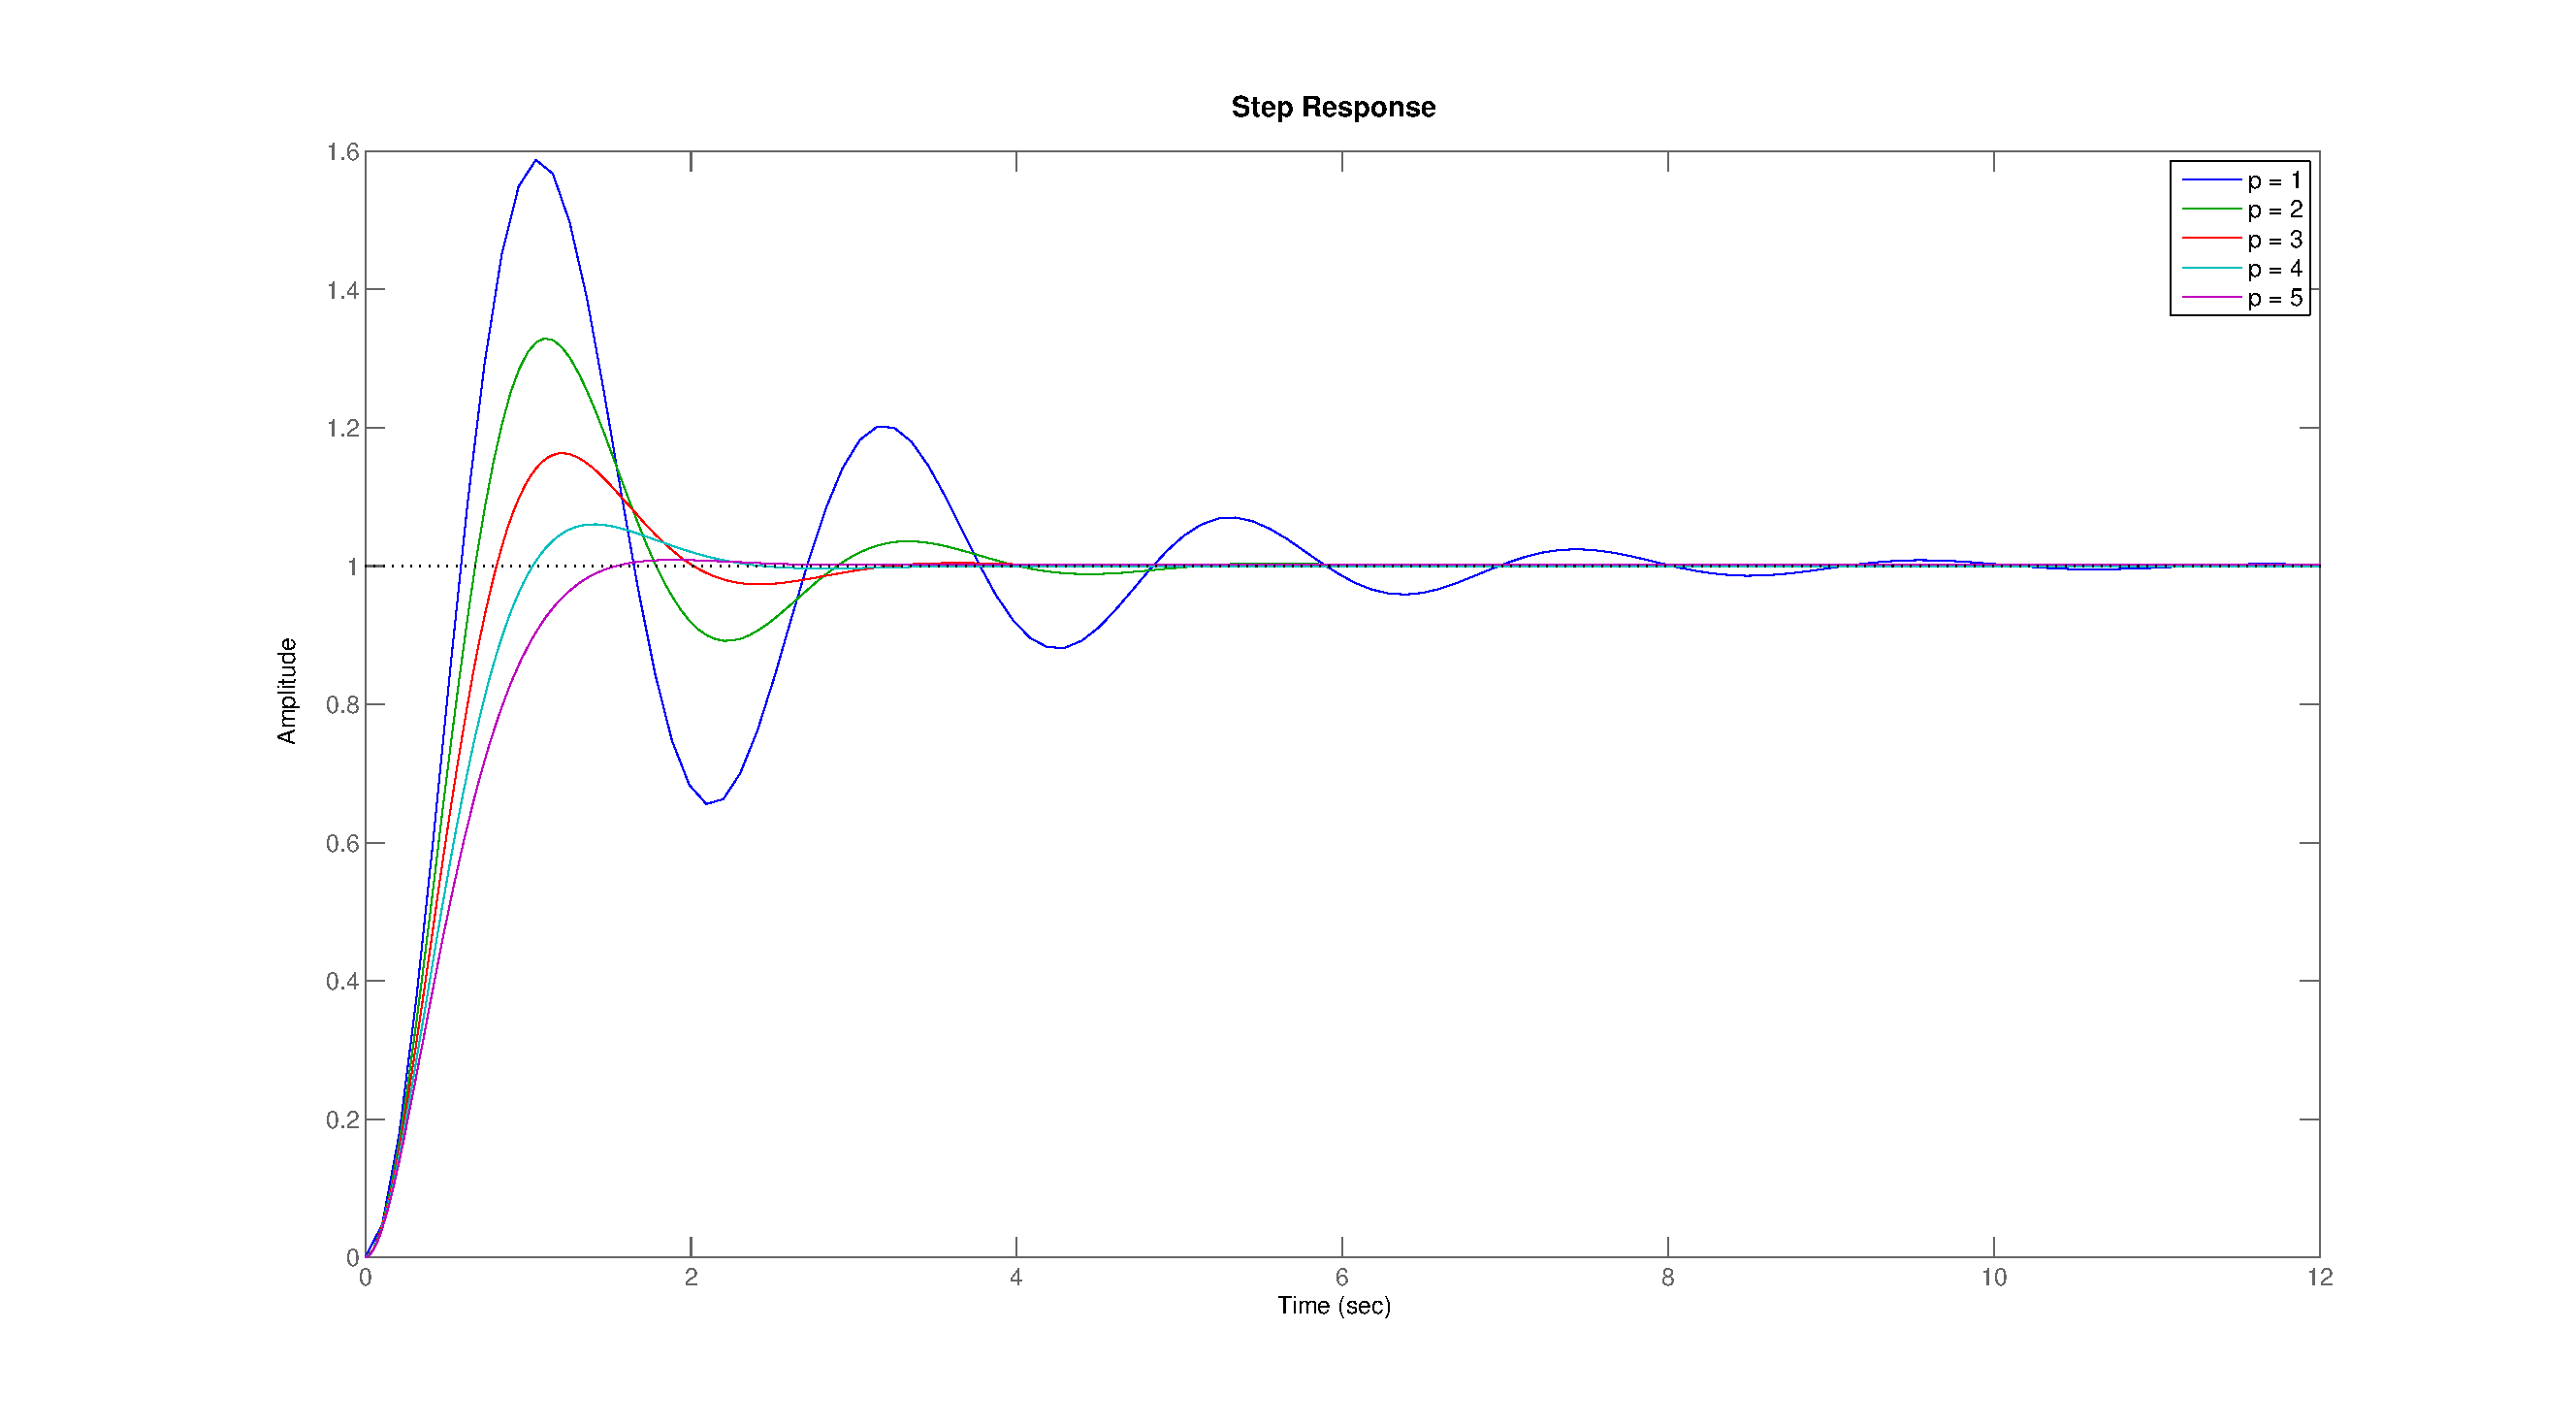
\includegraphics[width=0.95\textwidth]{imgs/questao1/resp_deg_mf}
    \caption{Resposta ao degrau unitário do sistema em malha fechada.}
    \label{fig:resp_deg_mf}
\end{figure}

Para \citeasnoun{dorf:2009}, a sensibilidade de um sistema é definida como sendo
a razão entre a variação percentual da função de transferência do sistema e a
variação percentual da função de transferência do processo (ou parâmetro). Ou
seja, para uma dada função de transferência do sistema $T(s)$, tem-se:

\begin{equation}
S = \frac{\Delta T(s)/T(s)}{\Delta G(s)/G(s)}
\end{equation}

No limite, para pequenas variações incrementais, tem-se:

\begin{equation}
S_G^T(s) = \frac{\partial T / T}{ \partial G / G} 
         = \frac{\partial T}{\partial G} \cdotp \frac{G}{T}
\end{equation}

Assim, para o parâmetro $p$ da função de transferência de malha fechada
obtida pela Eq. \ref{eq:G_MF_q1}, tem-se:

\begin{eqnarray}
S_p^G(s) & = & \frac{\partial G}{\partial p} \cdotp \frac{p}{G}\nonumber \\
         & = & \frac{0(s^2 + ps + 9) - 9(s)}{(s^2 + ps + 9)^2} \cdotp
               \frac{p}{\D\frac{9}{s^2 + ps + 9}}\nonumber\\
         & = & - \frac{9ps}{9(s^2 + ps + 9)}\nonumber\\
         & = & - \frac{ps}{s^2 + ps + 9}\label{eq:sensib}
\end{eqnarray}

Considerando $p = 1\text{,}\ 2\text{,}\ \ldots\text{,}\ 5$, obtém-se os
diagramas de Bode ilustrados pela Fig. \ref{fig:diag_bode_sensib}.

\begin{figure}[H]
\centering
    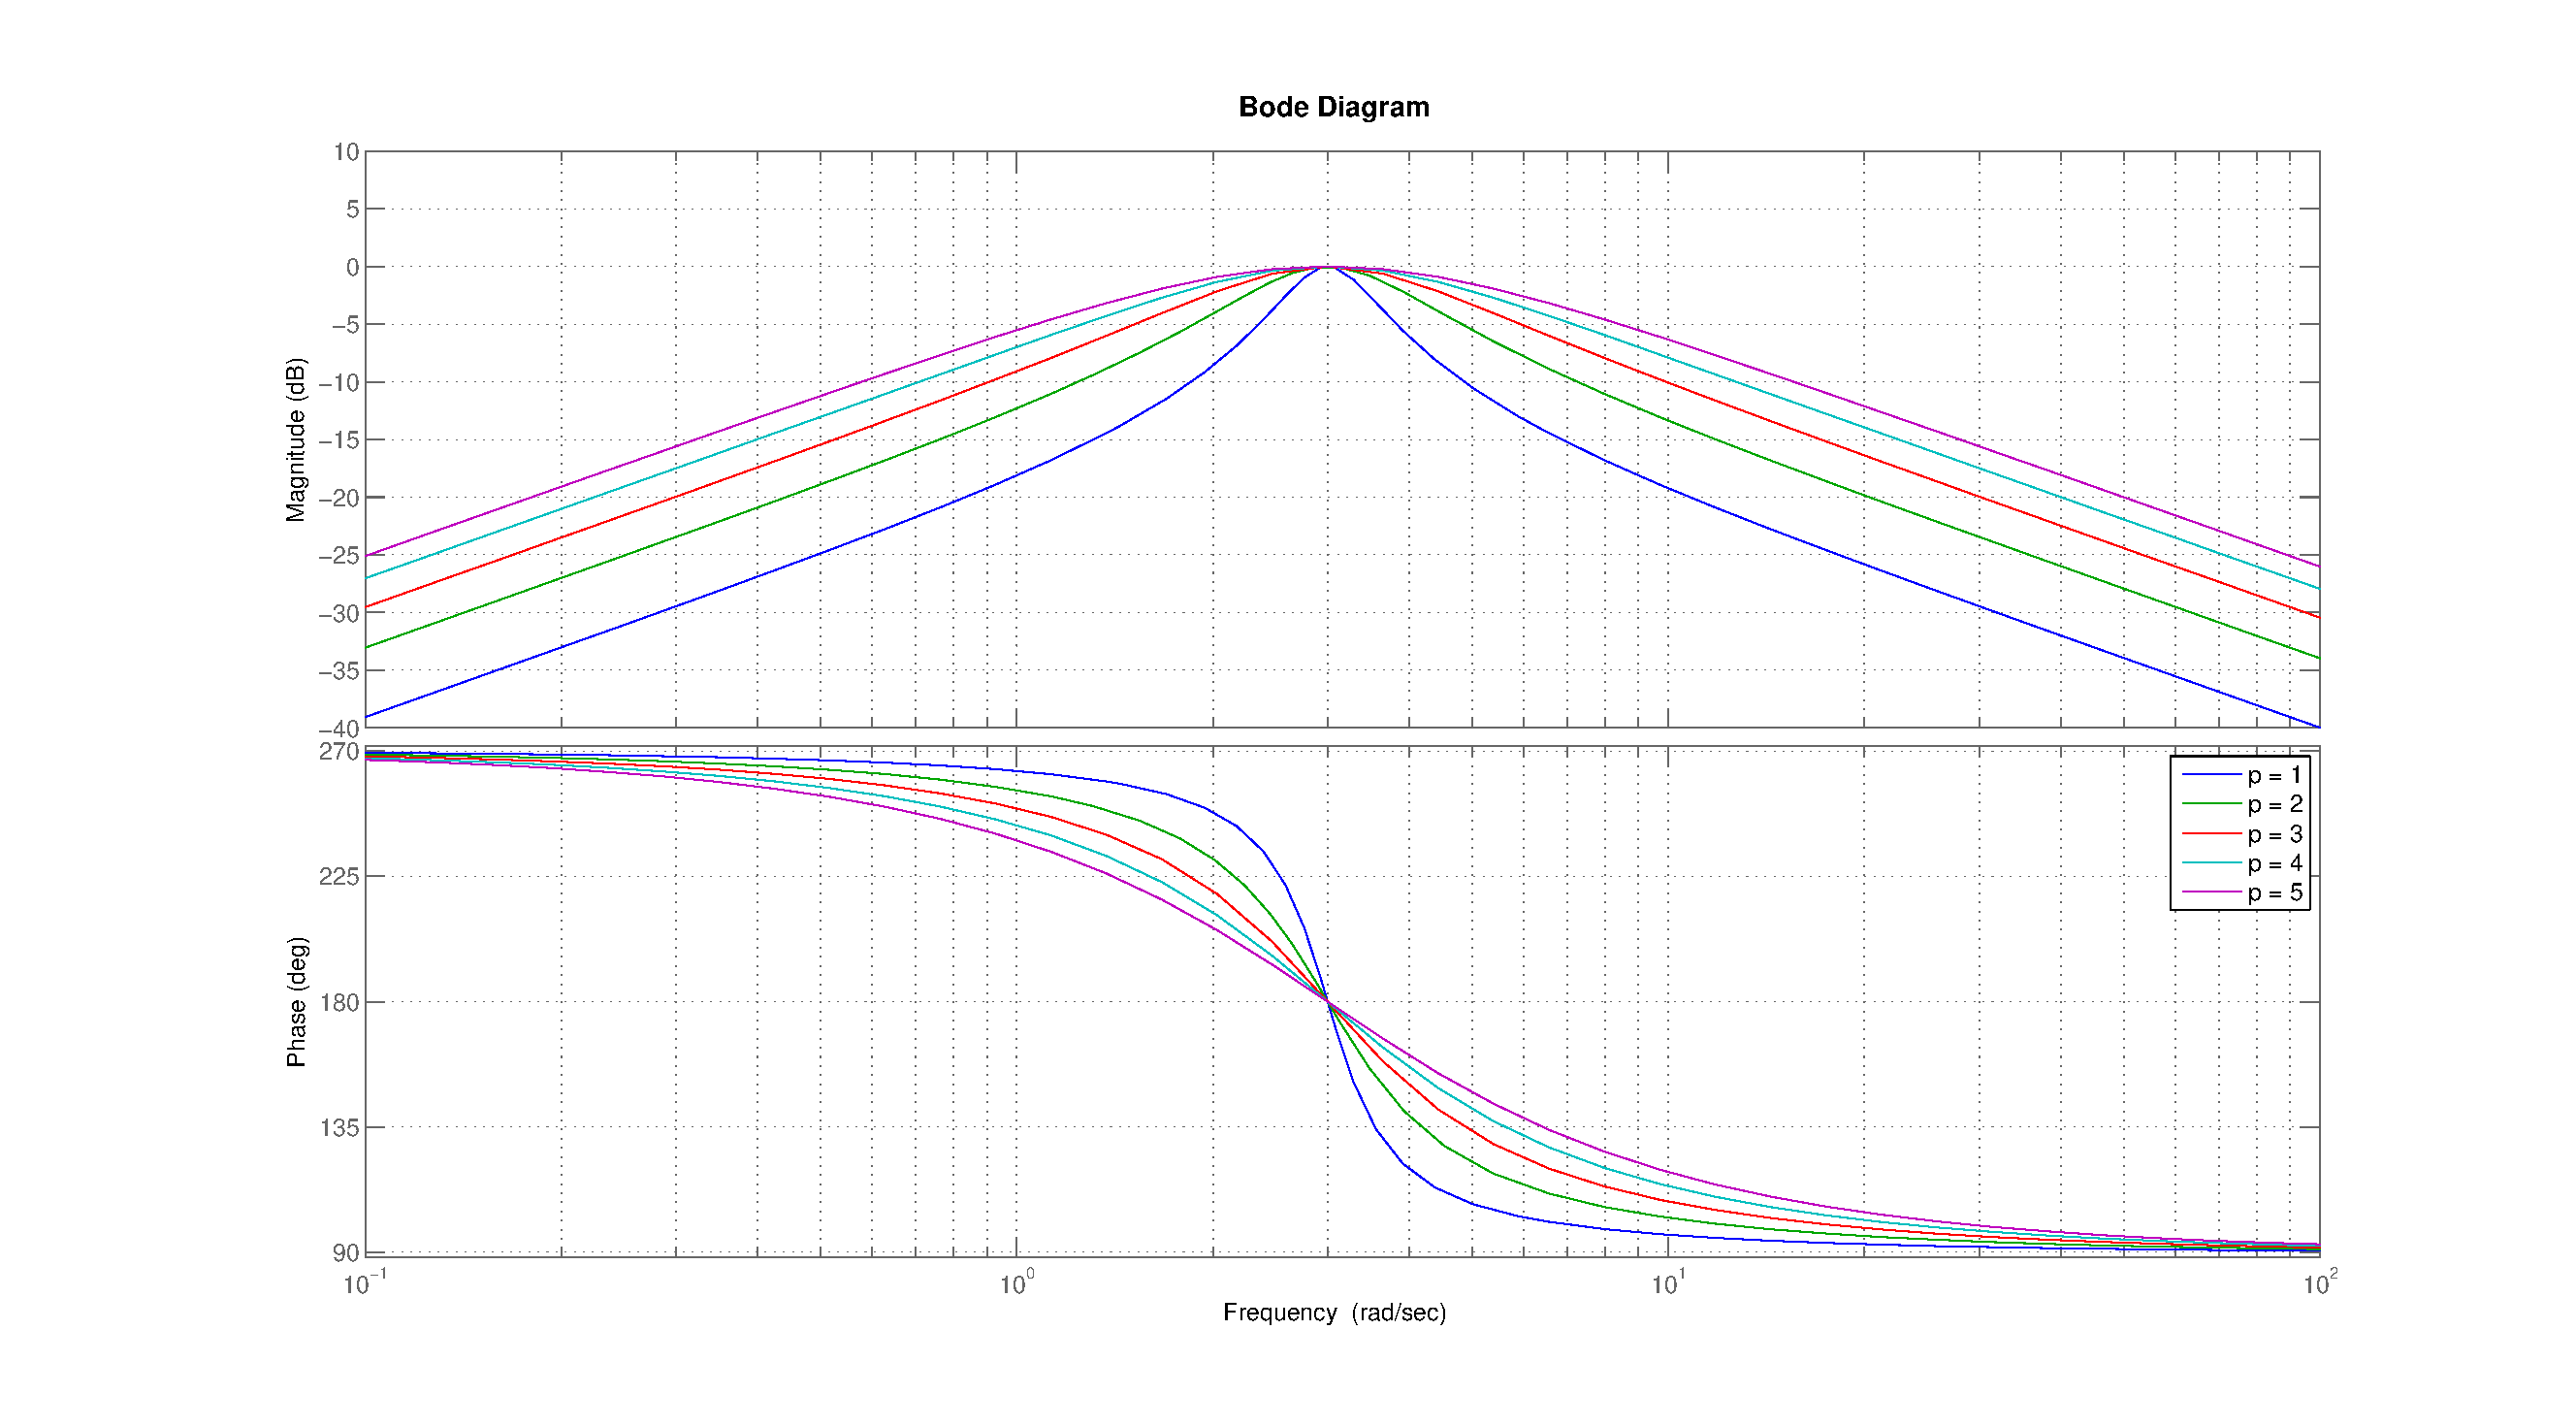
\includegraphics[width=0.95\textwidth]{imgs/questao1/bode_sensib}
    \caption{Diagrama de bode para a Eq. \ref{eq:sensib}.}
    \label{fig:diag_bode_sensib}
\end{figure}

Tendo em vista que os sistemas robustos são aqueles que apresentam baixa
sensibilidade à variação dos parâmetros, pode-se dizer que, para os sistemas
mais robustos, a sensibilidade ideal é tão baixa quanto possível.

Analisando então as curvas de módulo da Fig. \ref{fig:diag_bode_sensib},
verifica-se que todas elas apresentam baixa sensibilidade para frequências
baixas e altas. Entretanto, observa-se uma equivalência quanto a sensibilidade
para frequências em torno de 3 rad/s.

Fazendo uma análise comparativa, pode-se dizer que o sistema é estável para a
faixa de variação do parâmetro $p$ e que apresenta maior robustez quando $p =
1$, pois é a curva que apresenta os menores valores dentre as curvas de módulo
do diagrama de Bode. Contudo, observa-se que o sistema se torna bastante
oscilatório para esse valor de $p$, o que era esperado, uma vez que a relação
desempenho/robustez é inversa.

O {\it script} do Matlab\textsuperscript{\textregistered} desenvolvido para a
resolução dessa questão pode ser encontrado no Apêndice \ref{ap:cod_q1}.

\pagebreak
% UFRN - CT - DCA
% Controle Avançado - Lista 1
% Questão 2
% Autor: Cristiano Gurgel de Castro <crisgc@dca.ufrn.br>

\section*{Questão 2}

\textit{Um sistema com realimentação unitária tem a seguinte função de
transferência de malha aberta:}

\begin{flalign*}
G(s) = \frac{s+r}{(s+p)(s+q)}
\end{flalign*}

\noindent \textit{em que $0 \leq p \leq 5$, $0 \leq q \leq 1$ e $1 \leq r \leq
2$.  Selecione os parâmetros (todos reais) de um controlador atraso-avanço de
fase, de forma que o sistema em malha fechada tenha um desempenho robusto. Faça
simulações no \emph{Matlab} para comprovar o desempenho do sistema.}

\vspace{0.5cm}

\noindent{\bf Resolução:}

\vspace{0.25cm}

Para efeitos de análise e projeto dos controladores, utilizamos os valores médio
de cada um dos parâmetros, a saber $\vmedio{r} = 1,5$, $\vmedio{p} = 4$ e
$\vmedio{q} = 0,5$ e a função de transferência de malha aberta é escrita como

\begin{flalign}
\vmedio{G}(s) & = \frac{s+\vmedio{r}}{(s+\vmedio{p})(s+\vmedio{q})}  =
\frac{s+1,5}{(s+4)(s+0,5)} = {\frac{1,5+s}{2+4,5s+s^{2}}} \label{eq:q2:gma}
\end{flalign}

\noindent e o lugar das raízes para esse sistema é mostrado a seguir:

\begin{figure}[htb]
\centering
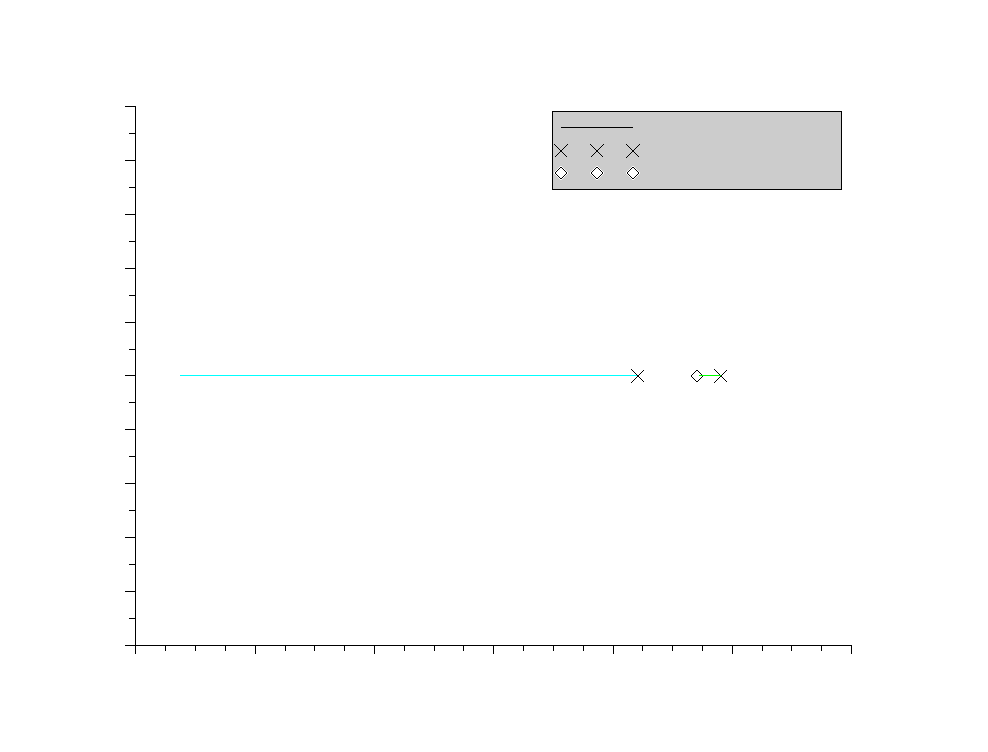
\includegraphics[width=0.8\textwidth]{imgs/questao2/rlocus_gma}
\caption{Lugar das raízes para os valores médios ($\vmedio{G}(s)$).}
\label{fig:q2:rlocus_gma}
\end{figure}

% TODO(crisgc): colocar diagrama de bloco com a malha fechada
Como um passo inicial, fechamos a malha e testamos a sua robustez segundo os
polinômios de Kharitonov. A função de transferência em malha fechada é mostrada a
seguir.

\begin{flalign}
G_{\text{MF}}(s) & = \frac{s+r}{(s+p)(s+q) + s+r} =
\frac{s+r}{s^{2}+\underbrace{(p+q+1)}_{a_1}s +
\underbrace{pq+r}_{a_0}} \nonumber \\
\vmedio{G_{\text{MF}}}(s) & = {\frac{1,5+s}{3,5+5,5s+s^{2}}} =
\frac{1,5+s}{(s+4,7656)(s+0,7344)} \quad
\bigtriangleup
\quad \text{Tomando os valores médios} \label{eq:q2:gmf}
\end{flalign}

Analisando a função de transferência de malha fechada, temos que:

\begin{flalign*}
a_0 &= pq+r & \alpha_0 & = \mymin{p}\mymin{q} + \mymin{r} = 1 \quad 
&\beta_0 &= \mymax{p}\mymax{q} + \mymax{r} = 7 \\
a_1 &= p + q + 1 & \alpha_1 &= \mymin{p} + \mymin{q} + 1 = 4 \quad
&\beta_1 &=\mymax{p} + \mymax{q} + 1 = 7
\end{flalign*}

Os quatro polinômios retirados do \textit{Teorema de Kharitonov} para o teste da
estabilidade são os seguintes:

\begin{flalign*}
q_0 & = \alpha_0 + \alpha_1s + s^{2} = 1 + 4s + s^{2} = (s + 3,7321)(s + 0,2679) \\ 
q_1 & = \alpha_0 + \beta_1s + s^{2} = 1 + 7s + s^{2} = (s + 6,8541)(s + 0,1459)\\ 
q_2 & = \beta_0 + \alpha_1s + s^{2} = 7 + 4s + s^{2} = (s + 2 + 1,7321i)(s + 2 -
1,7321i)\\ 
q_3 & = \beta_0 + \beta_1s + s^{2} = 7 + 7s + s^{2} = (s + 5,7913)(s + 1,2087)\\ 
\end{flalign*}

Logo como nenhum polo do sistema está situado no semiplano direito, ou seja,
todos os polos tem parte real negativa, o sistema é estável para qualquer valor
dos parâmetros dentro do seus intervalos de variação. Calculamos então o valor
final da resposta ao degrau unitário para avaliar seu valor no regime
permanente:

\begin{flalign*}
\lim_{t \tende \infty}{y(t)} & = \lim_{s \tende 0}sY(s) \\
Y(s) & = R(s)\vmedio{G_{\text{MF}}}(s) = \frac{1}{s}\frac{1,5+s}{3,5+5,5s+s^{2}} \\
\lim_{t \tende \infty}{y(t)} & =  \lim_{s \tende
0}s\frac{1}{s}\frac{1,5+s}{3,5+5,5s+s^{2}} = \frac{1,5}{3,5} = \frac{3}{7}
\approx 0,429
\end{flalign*}

\noindent o que condiz com o valor obtido por simulação (ver figura
\ref{fig:q2:resposta_gmf}).

\begin{figure}[htb]
\centering
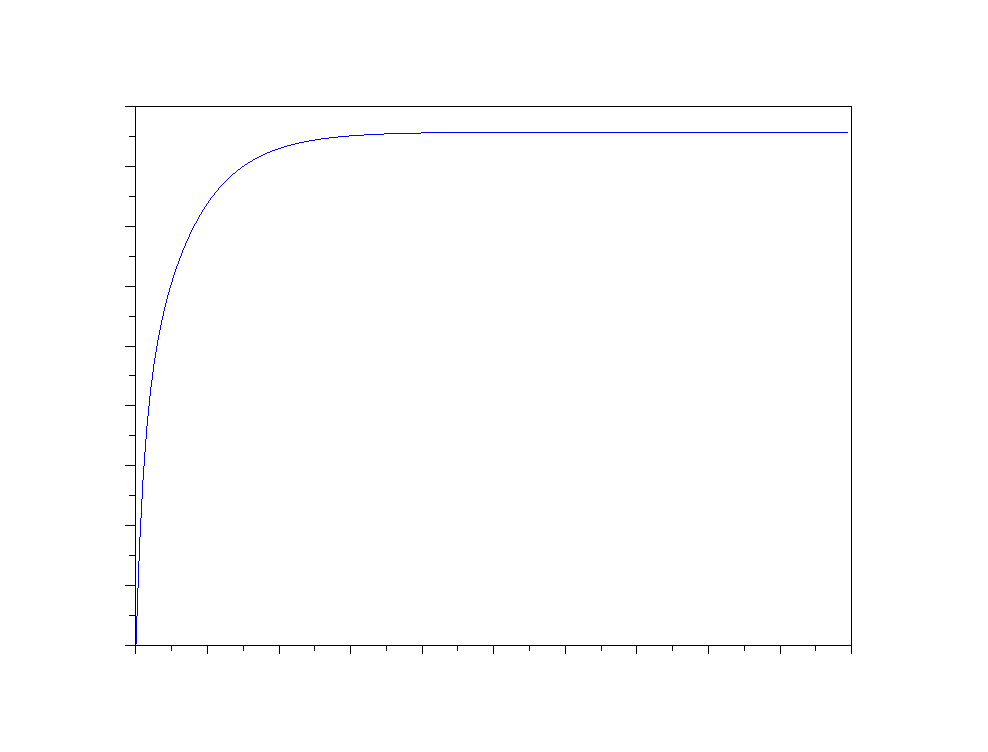
\includegraphics[width=0.8\textwidth]{imgs/questao2/resposta_gmf}
\caption{Resposta do sistema em malha fechada ao degrau unitário para um tempo de $20$s.}
\label{fig:q2:resposta_gma}
\end{figure}

O primeiro passo do projeto foi, então, um projeto de um controlador em atraso
de fase \cite{dorf:2009,maitelli2002} para a melhora do erro de regime a uma entrada
em degrau. A constante de erro de posição do sistema que obtivemos é dado por
$K_{p} = G(0) = 0,75$, o que resulta no erro de regime previamente calculado.
Decidimos adotar uma tolerância do erro de regime de aproximadamente  $1\%$ e
projetamos um compensador de modo que a constante de erro ficasse em $K'_p = 100$. O
controlador em atraso de fase tem a seguinte função de transferência:

% TODO(crisgc): Colocar a figura da resposta em malha fechada simples
\begin{flalign*}
G_c(s) & = k_c \frac{s+z_c}{s+p_c} \quad \text{onde} \quad |z_c| > |p_c| \\
\end{flalign*}

Portanto para obter a constante de erro desejada teríamos então que fazer:

\begin{flalign}
\underbrace{K'_{p}}_{100} & = G_c(0)G(0) = G_c(0)K_{p} = k_c \frac{z_c}{p_c}
\underbrace{K_{p}}_{0,75} \nonumber \\
k_c \frac{z_c}{p_c}& = \frac{100}{0,75} =  \frac{400}{3} \approx 133,333
\label{eq:q2:comp_atraso}
\end{flalign}

Como o polo dominante do sistema de malha aberta está localizado em $-0,5$ (ver
equação \ref{eq:q2:gma}) decidimos por alocar o zero do controlador à sua
direita, para que a interferência no regime transitório não seja muito
significante, fizemos então $z_c = 0,3$, optamos em um primeiro momento não
adicionar o ganho no controlador, portante fizemos $k_c = 1$. O polo, calculado
a partir de \ref{eq:q2:comp_atraso} foi então $p_c = 0,0022$. 

A função de transferência em malha fechada do sistema, $G_{\text{cMF}}$ (ver
figura \ref{fig:q2:malha_comp}) já com o controlador pode ser obtida através da
redução do diagrama de blocos e é mostrada a seguir:

\begin{figure}[htb]
\centering
\scalebox{0.7}{\input{imgs/questao2/compensador_malha.pstex_t}}
\caption{Diagrama de blocos para o sistema com o compensador.}
\label{fig:q2:malha_comp}
\end{figure}

\begin{flalign}
G_\text{cMF}(s) & = \frac{G_c(s)G(s)}{1 + G_c(s)G(s)} =
\frac{k_c(s+z_c)(s+r)}{k_c(s+z_c)(s+r) + (s+p)(s+q)(s+p_c)} \nonumber \\
& = \frac{k_cs^{2} + k_c(z_c + r)s + k_crz_c}{s^{3} + \underbrace{[k_c + p_c +
(p+q)]}_{a_2}s^{2} +
\underbrace{[k_c(r+z_c) + p_c(p+q)+pq]}_{a_1}s + \underbrace{rz_c + pqp_c}_{a_0}
} \label{eq:q2:testeKharitonov}
\end{flalign}

Testamos a estabilidade do sistema segundo o \textit{teorema de Kharitonov}
utilizando o o script mostrado no apêndice \ref{ap:q2:testeKharitonov}.
Os quatro polinômio para os valores calculador do controlador, a saber $z_c = 0,3$, $k_c 
= 1$ e $p_c = 0,0022$, são os seguintes:

\begin{flalign*}
q_1 & = 0,3+1,3066s+7,0022s^{2}+s^{3} \\
q_2 & = 0,3+7,3132s+7,0022s^{2}+s^{3} \\
q_3 & = 0,611+1,3066s+5,0022s^{2}+s^{3} \\
q_4 & = 0,611+7,3132s+5,0022s^{2}+s^{3}
\end{flalign*}

\noindent e os polos de cada um desses polinômios podem ser visualizados na
seguinte matriz, onde cada coluna é referente a um polinômio. 

\begin{flalign*}
\begin{pmatrix}-0,093+0,188i&-0,043&-0,124+0,336i&-0,089\cr
-0,093-0,188i&-1,223&-0,124-0,336i&-2,457+0,917i\cr
-6,817&-5,736&-4,754&-2,457-0,917i\cr \end{pmatrix}
\end{flalign*}

\noindent logo podemos ver que o controlador desenvolvido é robusto para a faixa
estabelecida de variação dos parâmetros. E o resultado da resposta ao degrau com
o controlador pode ser visualizada na figura \ref{fig:q2:resposta_gcomp1}.
Através da análise da figura podemos ver que embora o desempenho do regime
permanente tende para o valor desejado (próximo a 1), a demora do sistema na
subida pode ser um problema que precisa ser evitado.
 
\begin{figure}[htb]
\centering
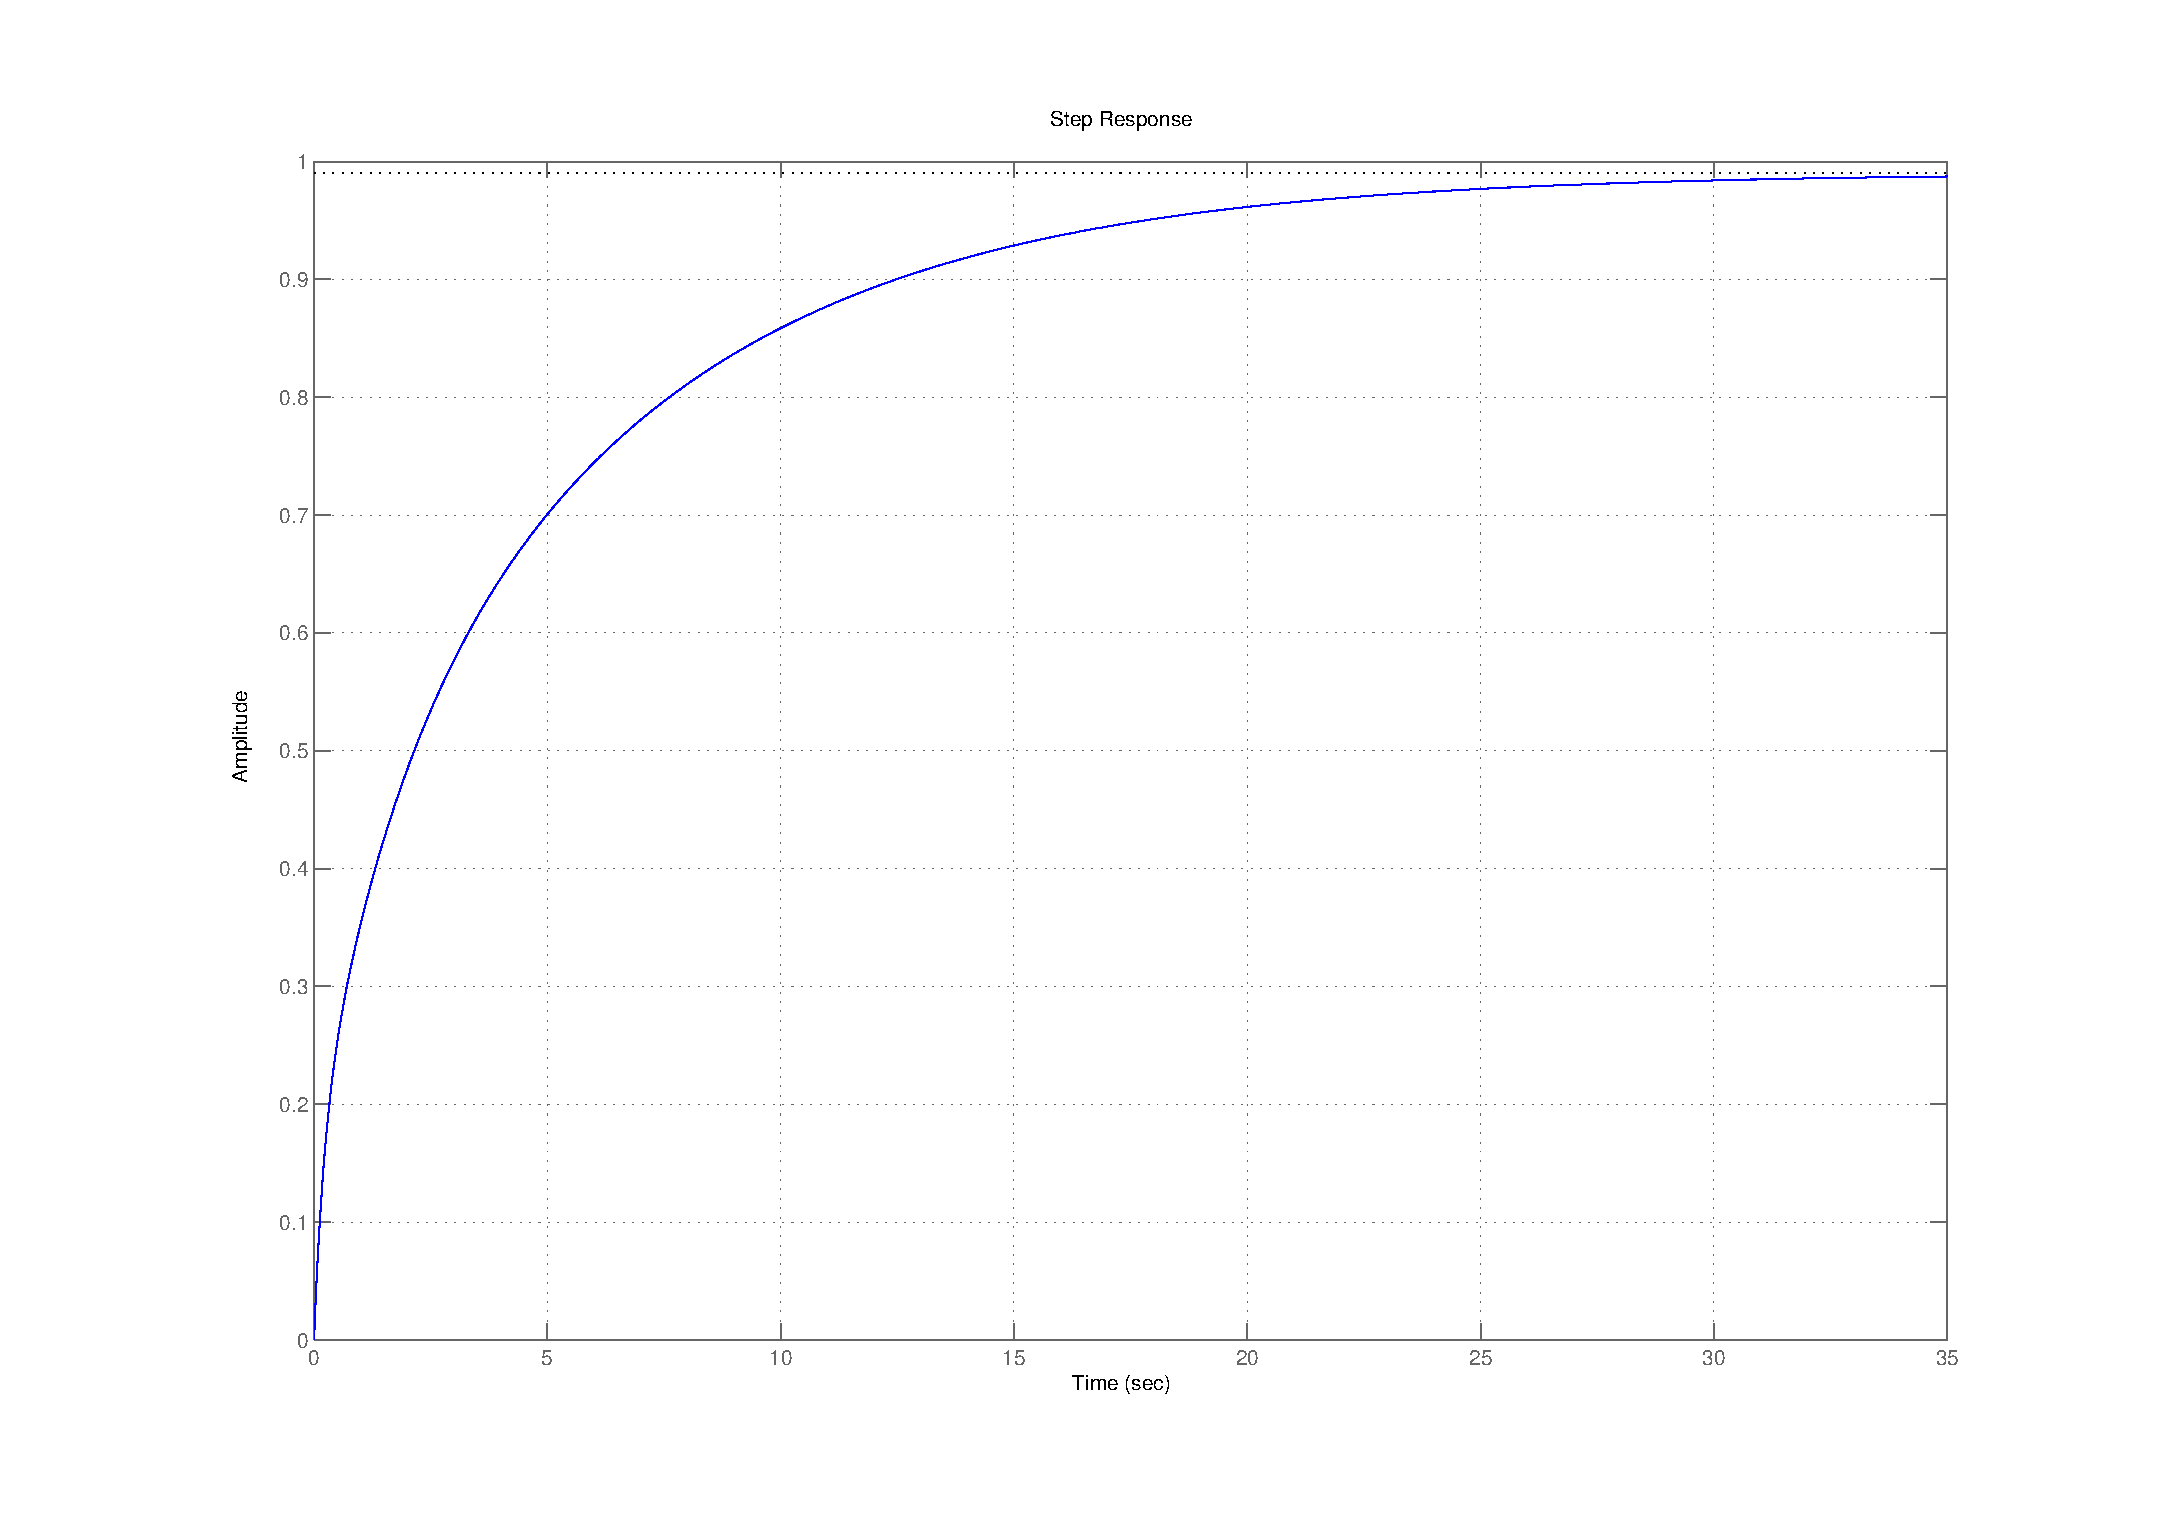
\includegraphics[width=0.8\textwidth]{imgs/questao2/resposta_gcomp1}
\caption{Resposta ao degrau para o controlador $G_c(s) = \frac{s+0,3}{s+0,0022}$}
\label{fig:q2:resposta_gcomp1}
\end{figure}

Então, para evitar esse problema, analisamos mais o lugar das raízes do sistema
em malha aberta com o controlador (ver figura \ref{fig:q2:rlocus_gcomp1}), e,
para melhorar o desempenho do tempo de subida decidimos por aumentar o ganho do
sistema, distanciando, dessa forma, os polos do eixo imaginário, dessa forma
tornando o sistema mais rápido. Testamos com um ganho para o controlador $k_c =
20$ e obtivemos, a resposta para o sistema em malha fechada mostrada na figura
\ref{fig:q2:resposta_gcomp2}.

\begin{figure}[htb]
\centering
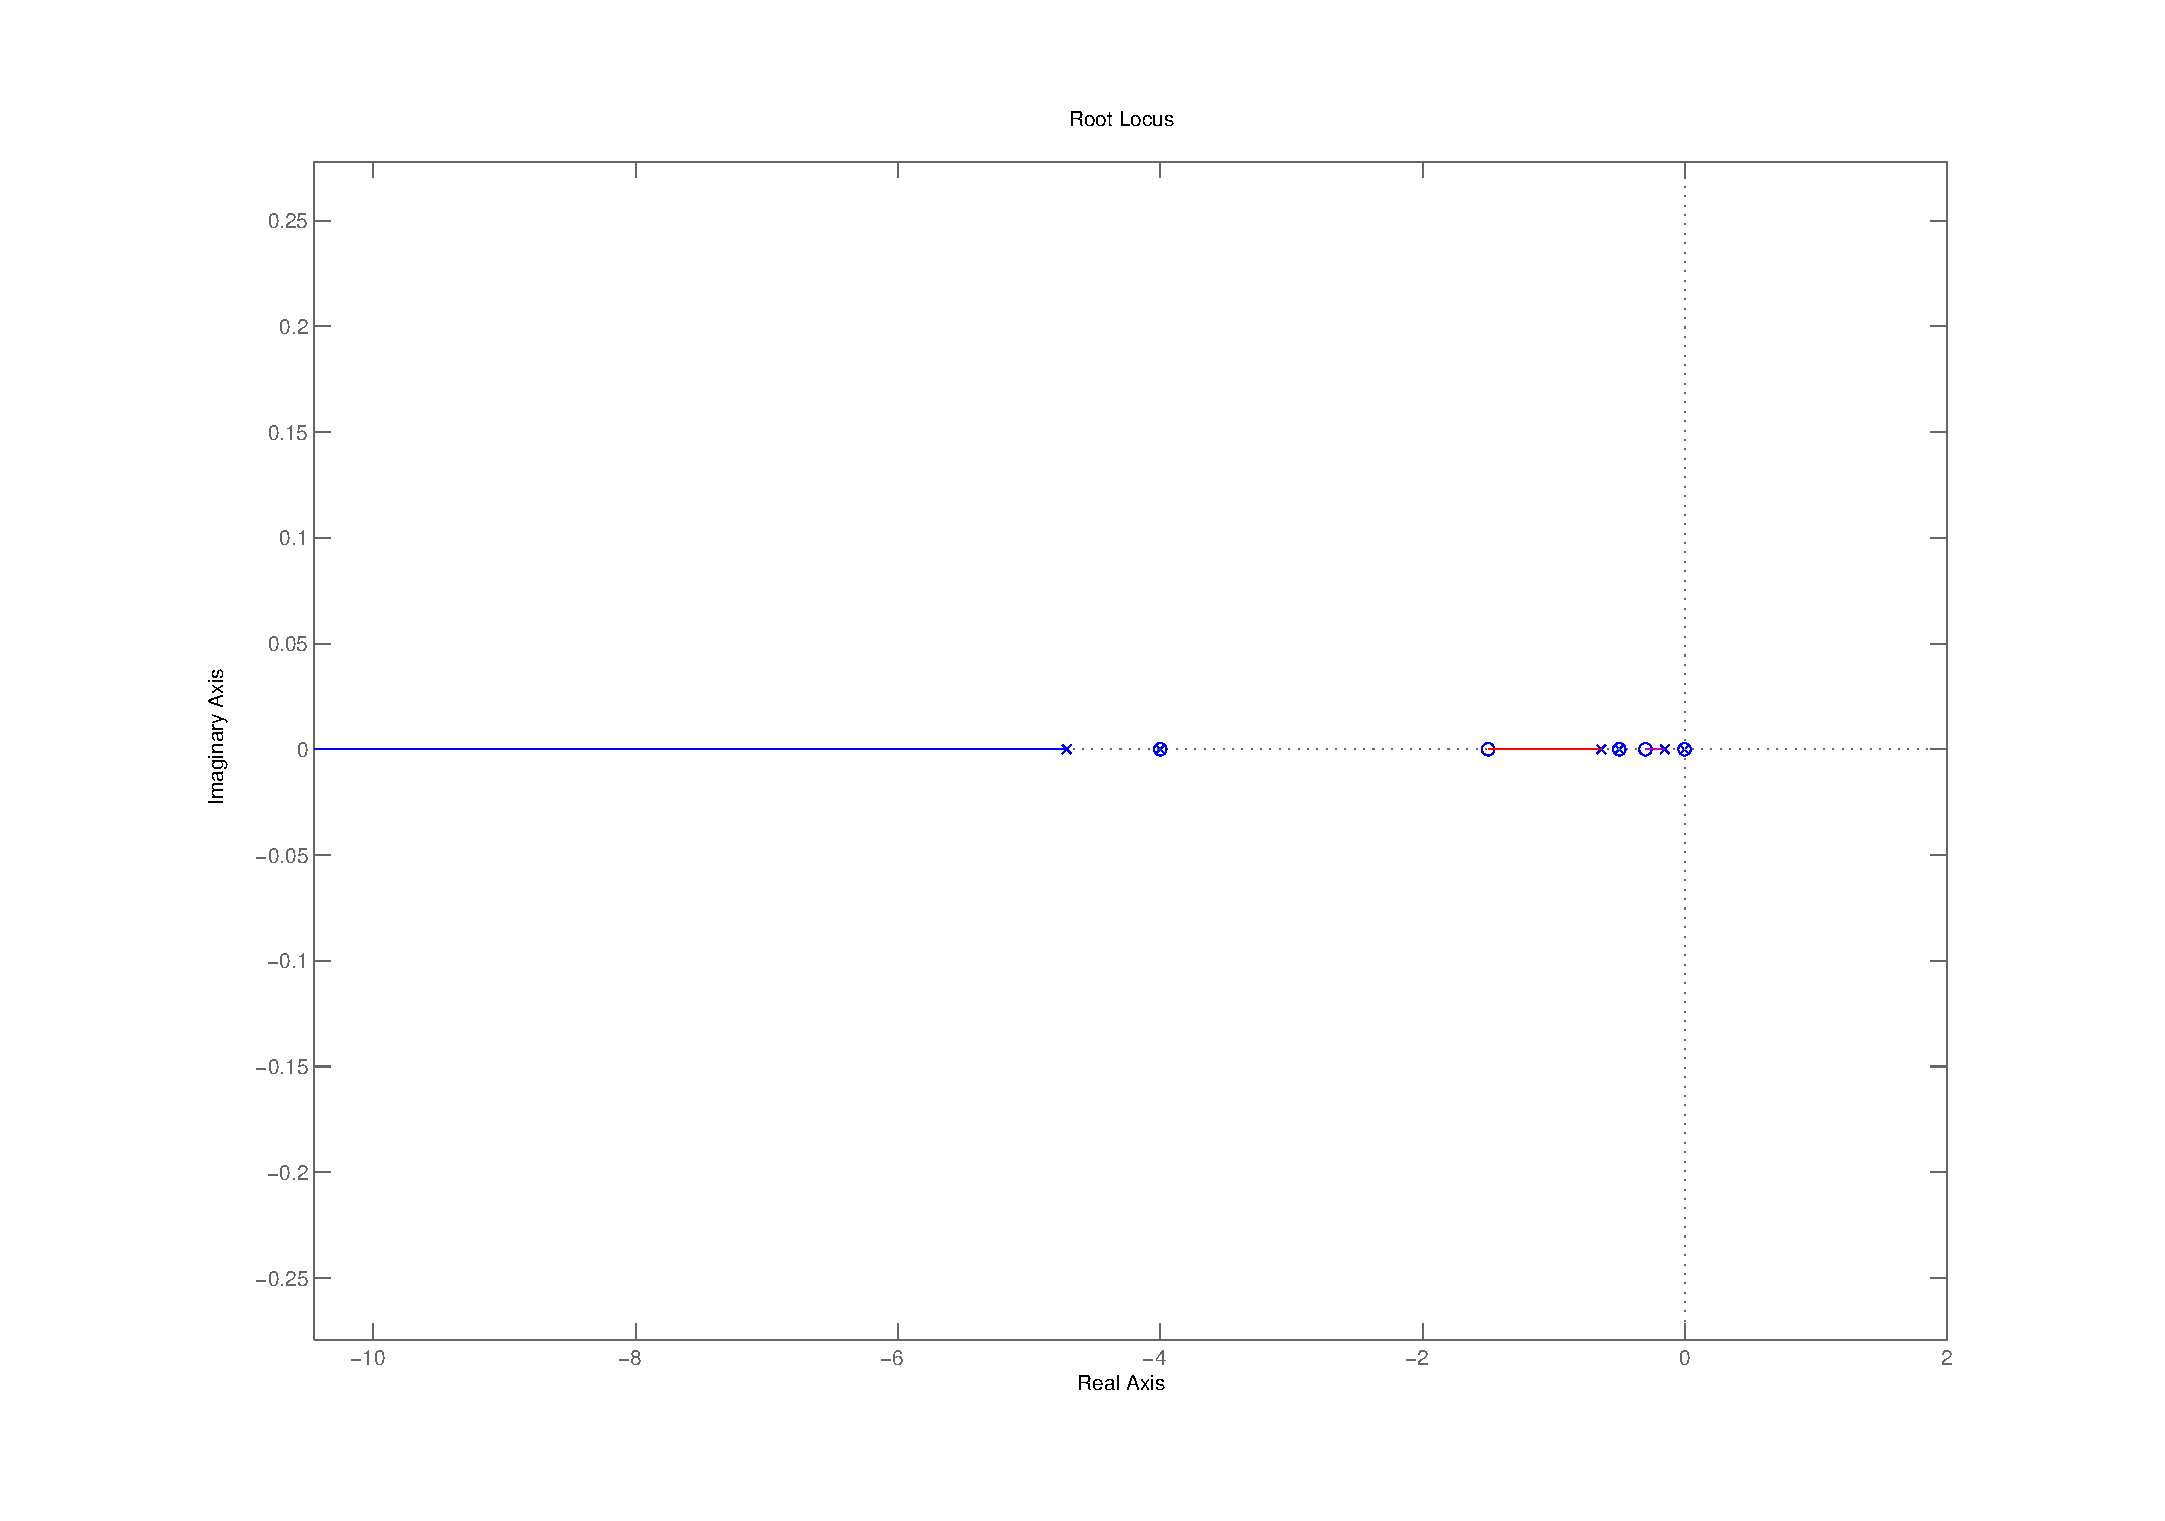
\includegraphics[width=0.8\textwidth]{imgs/questao2/rlocus_gcma}
\caption{Lugar das raízes para o sistema com o controlador $G_c(s)$}
\label{fig:q2:rlocus_gcomp1}
\end{figure}
 
\begin{figure}[H]
\centering
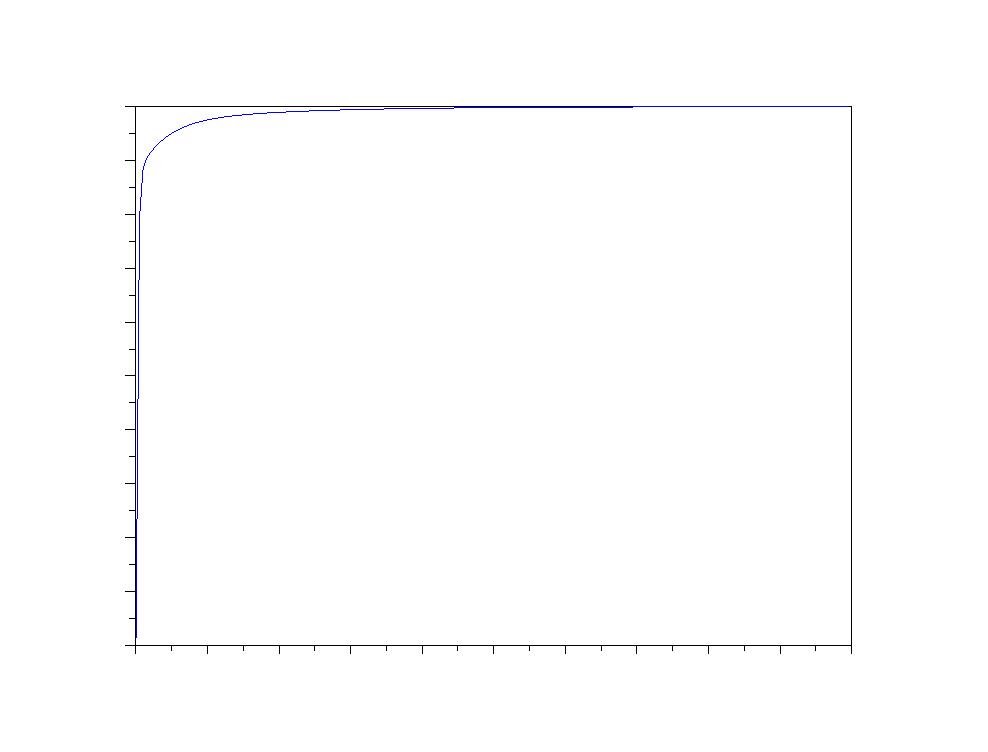
\includegraphics[width=0.8\textwidth]{imgs/questao2/resposta_gcomp2}
\caption{Reposta do sistema com o controlador $G_c(s) = 20\frac{s+0,3}{s+0,0022}$ }
\label{fig:q2:resposta_gcomp2}
\end{figure}

Podemos visualizar a melhora substancial no tempo de subida do sistema. Testamos
então a estabilidade do sistema para a faixa de variação de parâmetros mais uma
vez através dos polinômios de Kharitonov (ver equação
\ref{eq:q2:testeKharitonov} e o apêndice \label{ap:q2:testeKharitonov}) e
obtivemos os seguintes polinômios:

\begin{flalign*}
q_1 & = 0.3+26.0066s+26.0022s^{2}+s^{3} \\
q_2 & = 0.3+51.0132s+26.0022s^{2}+s^{3} \\
q_3 & = 0.611+26.0066s+24.0022s^{2}+s^{3} \\
q_4 & = 0.611+51.0132s+24.0022s^{2}+s^{3}
\end{flalign*}

\noindent e as suas raízes:

\begin{flalign*}
\begin{pmatrix}-0.012&-0.006&-0.024&-0.012\cr -1.03&-2.131&-1.112&-2.343\cr
-24.961&-23.865&-22.866&-21.647\cr \end{pmatrix}
\end{flalign*}

O sistema é estável na faixa de variação dada dos parâmetros de $G(s)$. Logo o
controle é robusto. Como a resposta em regime permanente como em
regime transitório é satisfatória, o controlador em atraso de fase foi
suficiente para o projeto do sistema, e a parte em avanço de fase não foi
projetada. O controlador projetado é portanto:

\begin{flalign*}
G_c(s) = 20\frac{s+0,3}{s+0,0022}
\end{flalign*}

% TODO(crisgc): Colocar o desempenho do controlador para alguns valores
% "randômicos" da função de transferência

\pagebreak
% Universidade Federal do Rio Grande do Norte
% Programa de Pos-Graduacao em Engenharia Eletrica e de Computacao
% Lista 1 - Questao 1
% Autores: Anna Giselle Camara Dantas Ribeiro
%          Cristiano Gurgel de Castro
%          Diogo Leite Reboucas
%          Thiago Medeiros Barros

\chapter*{Questão 3}
% Enunciado
\noindent {\it Considere o sistema descrito pelo modelo}

\begin{equation}\label{eq:enunc_1}
\ddot{y} = -\dot{y} - y  + u 
\end{equation}

\noindent {\it com o modelo de referência}

\begin{equation}\label{eq:enunc_2}
\ddot{y}_m = -2\dot{y}_m - y_m  + u
\end{equation}

\noindent {\it Implementar um controlador MRAC e utilize como entrada uma onda
quadrada para avaliar o comportamento do sistema.}

\vspace{0.5cm}

\noindent{\bf Resolução:}

\vspace{0.25cm}

Dadas as Eqs. \ref{eq:enunc_1} e \ref{eq:enunc_2}, pode-se generalizá-las de
modo a obter as Eqs. \ref{eq:modelo} e \ref{eq:ref}.

\begin{eqnarray}
\ddot{y}(t) & = &-a\dot{y}(t) - by(t) + cu(t) \label{eq:modelo}\\
\ddot{y}_m(t) & = &-a_m\dot{y}(t) - b_my(t) + c_mr(t) \label{eq:ref}
\end{eqnarray}

A partir das Eqs. \ref{eq:modelo} e \ref{eq:ref}, deriva-se a Eq.
\ref{eq:lei_cont} referente a lei de controle:

\begin{equation}\label{eq:lei_cont}
u(t) = \theta_1r(t) - \theta_2\dot{y}(t) - \theta_3y(t)
\end{equation}

Essa equação mostra três parâmetros $\theta_1$, $\theta_2$ e $\theta_3$, que
foram escolhidos de maneira a satisfazer as seguintes condições:

\begin{equation}
\theta_1 = \frac{c_m}{c}
\qquad
\theta_2 = \frac{a_m - a}{c}
\qquad
\theta_3 = \frac{b_m - b}{c}
\end{equation}

A partir dessas condições, para a aplicação da regra {\it MIT} faz-se necessário
introduzir a variável erro $\epsilon = y - y_m$, na qual $y$ representa a saída
do sistema em malha fechada. Segundo tal regra, o mecanismo para ajuste de
parâmetros é dado por:

\begin{equation}
J(\theta) = \frac{\epsilon^2}{2}
\end{equation}

Minimizar o erro implica em minimizar $J(\theta)$. Por sua vez, para minimizar o
valor de $J$, troca-se os parâmetros na direção do gradiente negativo de $J$, de
tal maneira que:

\begin{equation}\label{eq:J}
\frac{d\theta}{dt} = -\gamma\ \frac{\partial J}{\partial \theta} = 
                     -\gamma\ \epsilon\ \frac{\partial \epsilon}
                                             {\partial \theta}
\end{equation}

Aplicando a Eq. \ref{eq:lei_cont} na Eq. \ref{eq:modelo}, tem-se:

\begin{eqnarray}
\ddot{y} & = & -a\dot{y} - by + c \left( \theta_1r - 
                                         \theta_2\dot{y} - 
                                         \theta_3y\right)\nonumber\\
\ddot{y} & = & -a\dot{y} - by + c\theta_1r - 
                                c\theta_2\dot{y} -
                                c\theta_3y\nonumber\\
\ddot{y} & = & -(a + c\theta_2)\dot{y} - (b + c\theta_3)y + c\theta_1r\nonumber
\end{eqnarray}

Considerando o operador diferencial $p = \frac{d}{dt}$, tem-se que:

\begin{eqnarray}
p^2y & = & - (a + c\theta_2)py - 
             (b + c\theta_3)y + 
             c\theta_1r\nonumber\\
y & = & \frac{c\theta_1}{p^2 + 
                         (a + c\theta_2)p + 
                         (b + c\theta_3)}r\label{eq:y}
\end{eqnarray}

Isolando $\theta_1$, tem-se:

\begin{equation}\label{eq:theta_1}
\theta_1 = \frac{y}{cr}\left[ p^2 + (a + c\theta_2)p + (b + c\theta_3) \right]
\end{equation}

A partir das Eqs. \ref{eq:y} e \ref{eq:theta_1}, obtém-se as Eqs.
\ref{eq:dtheta_1} a \ref{eq:dtheta_3}, referentes as derivadas com relação aos
parâmetros $\theta_1$, $\theta_2$ e $\theta_3$:

\begin{eqnarray}
\frac{\partial \epsilon}{\partial \theta_1} = \frac{\partial y}{\partial \theta_1} & = &
    \frac{c}{p^2 + (a + c\theta_2)p + (b + c\theta_3)}\ r 
    \label{eq:dtheta_1}\\
\frac{\partial \epsilon}{\partial \theta_2} = \frac{\partial y}{\partial \theta_2}  & = &
    -\frac{cp}{p^2 + (a + c\theta_2)p + (b + c\theta_3)}\ y 
    \label{eq:dtheta_2}\\
\frac{\partial \epsilon}{\partial \theta_3} = \frac{\partial y}{\partial \theta_3}  & = &
    -\frac{c}{p^2 + (a + c\theta_2)p + (b + c\theta_3)}\ y 
    \label{eq:dtheta_3}
\end{eqnarray}

Uma vez que os parâmetros $a$, $b$ e $c$ podem não ser conhecidos, as Eqs.
\ref{eq:dtheta_1} a \ref{eq:dtheta_3} não podem ser utilizadas de maneira
direta. Entretanto, sabe-se que:

\begin{eqnarray}
p^2 + (a + c\theta_2)p + (b + c\theta_3) & \approx & 
p^2 + 
\left[a + c\left( \frac{a_m - a}{c} \right)\right]p + 
\left[b + c\left( \frac{b_m - b}{c} \right)\right] \nonumber\\ 
 & \approx & p^2 + a_mp + b_m \nonumber
\end{eqnarray}

Assim, pela Eq. \ref{eq:J}, obtém-se as Eqs. \ref{eq:dtheta_1dt} a
\ref{eq:dtheta_3dt}, em que o fator $\frac{c}{b_m}$ está incluso em $\gamma$:

\begin{eqnarray}
\frac{d\theta_1}{dt} & = & -\gamma\ \left(\frac{b_m}
                                             {p^2 + a_mp + b_m}\ r
                                  \right)\epsilon \label{eq:dtheta_1dt}\\
\frac{d\theta_2}{dt} & = & \gamma\ \left(\frac{b_m p}
                                            {p^2 + a_mp + b_m}\ y
                                 \right)\epsilon \label{eq:dtheta_2dt}\\
\frac{d\theta_3}{dt} & = & \gamma\ \left(\frac{b_m}
                                          {p^2 + a_mp + b_m}\ y
                               \right)\epsilon \label{eq:dtheta_3dt}
\end{eqnarray}

Para realizar a simulação do sistema, foram utilizados os parâmetros dados na
questão:

\begin{eqnarray}
a = 1 \qquad a_m = 2\\
b = 1 \qquad b_m = 1\\
c = 1 \qquad c_m = 1
\end{eqnarray}

Os diagramas de blocos do ambiente de simulação ({\it Simulink}) podem ser
vistos nas Figs. \ref{fig:q3_sistema} a \ref{fig:q3_sinal_cont}.

\begin{figure}[htb]
    \centering
    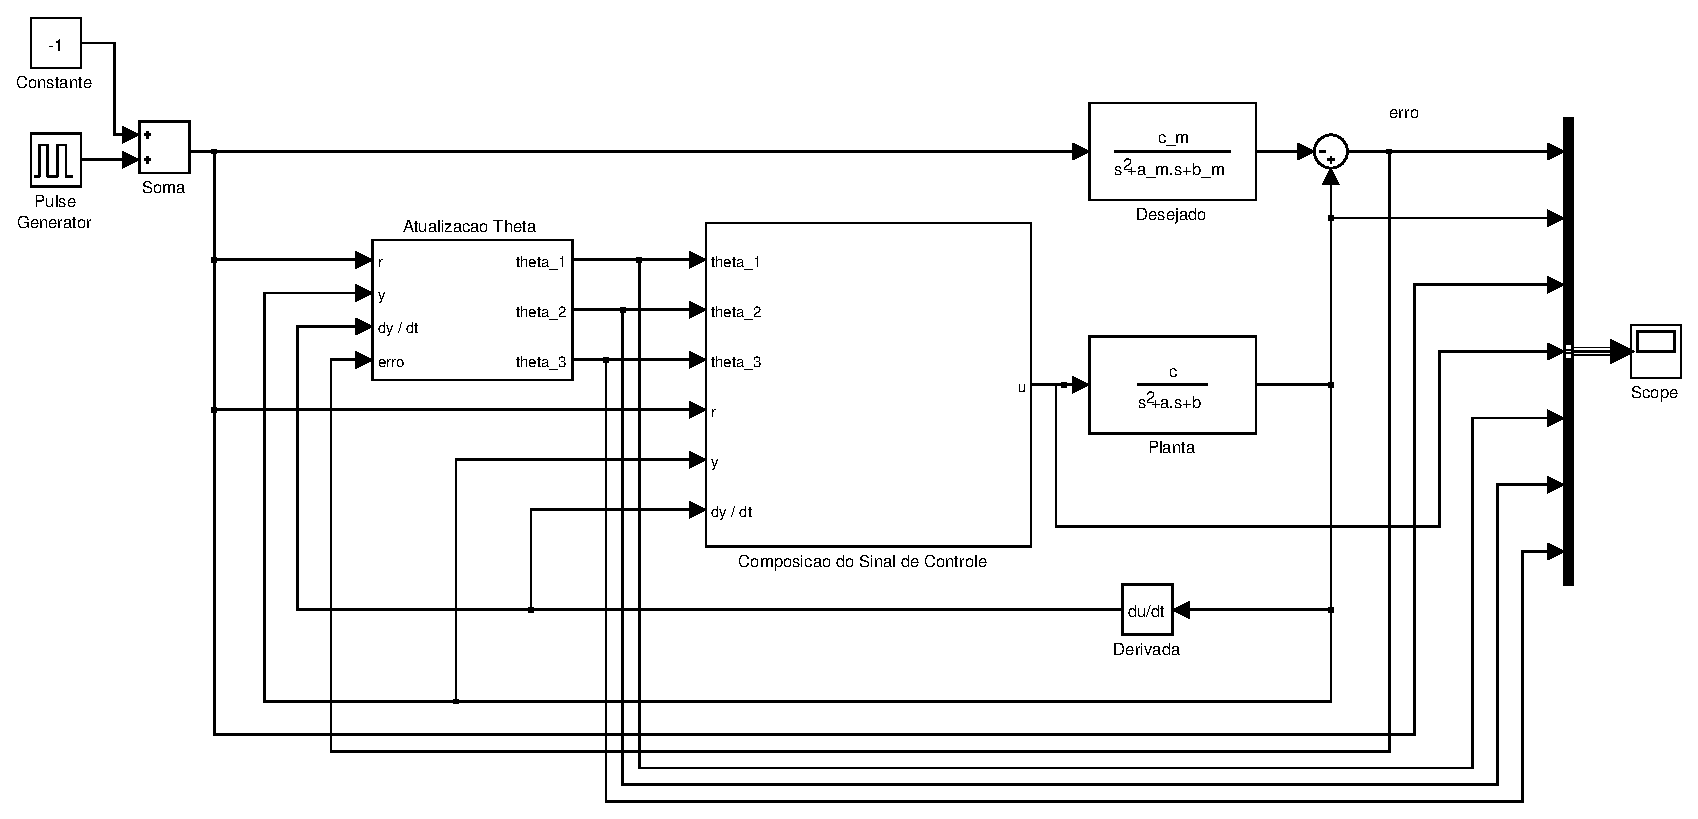
\includegraphics[width=0.95\textwidth]{imgs/questao3/sistema}
    \caption{Diagrama de blocos do sistema simulado.}
    \label{fig:q3_sistema}
\end{figure}

\begin{figure}[H]
    \centering
    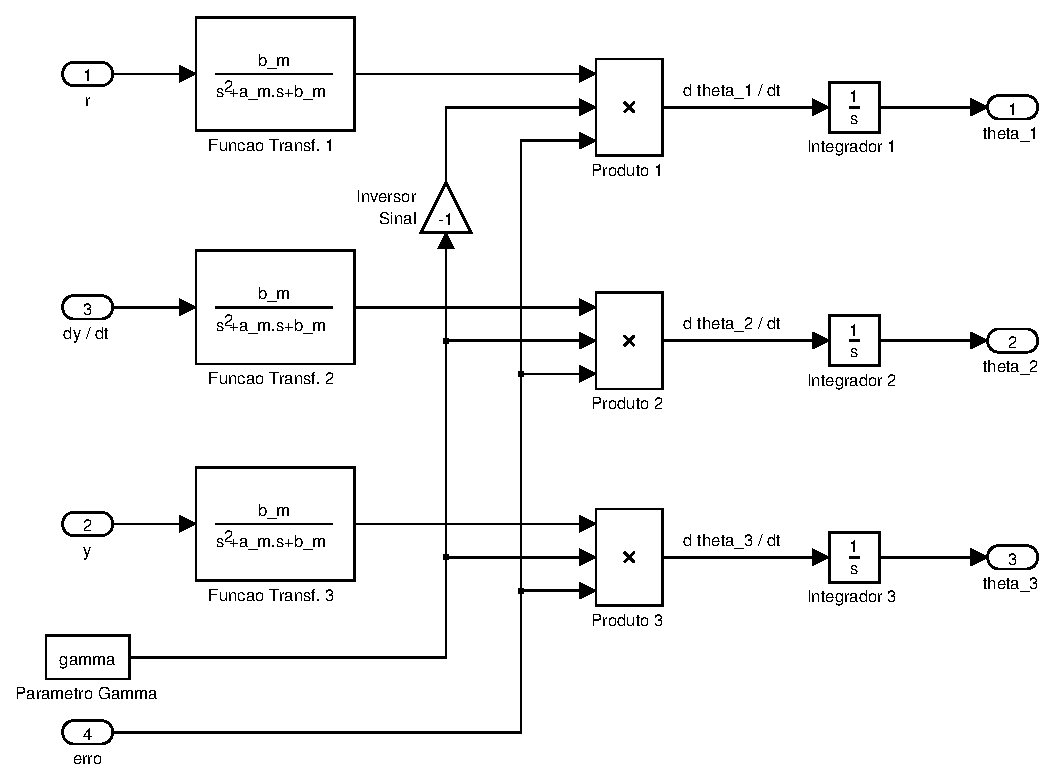
\includegraphics[width=0.8\textwidth]{imgs/questao3/theta}
    \caption{Diagrama de blocos do subsistema de atualização de $\theta$}
    \label{fig:q3_theta}
\end{figure}

\begin{figure}[H]
    \centering
    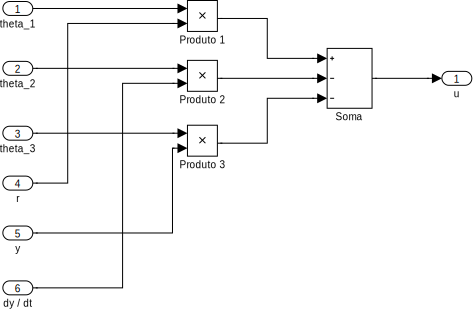
\includegraphics[width=0.6\textwidth]{imgs/questao3/sinal_controle}
    \caption{Diagrama de blocos do subsistema de composição do sinal de
             controle.}
    \label{fig:q3_sinal_cont}
\end{figure}

A simulação foi realizada para valores de $\gamma = 0.1\text{, } 0.2\text{, }
0.5\text{, } 0.7 \text{ e } 1.0$. Os resultados obtidos podem ser vistos nas
Figs. \ref{fig:q3_saida_gamma_0.1} a \ref{fig:q3_saida_gamma_1.0}

\begin{figure}[htb]
    \centering
    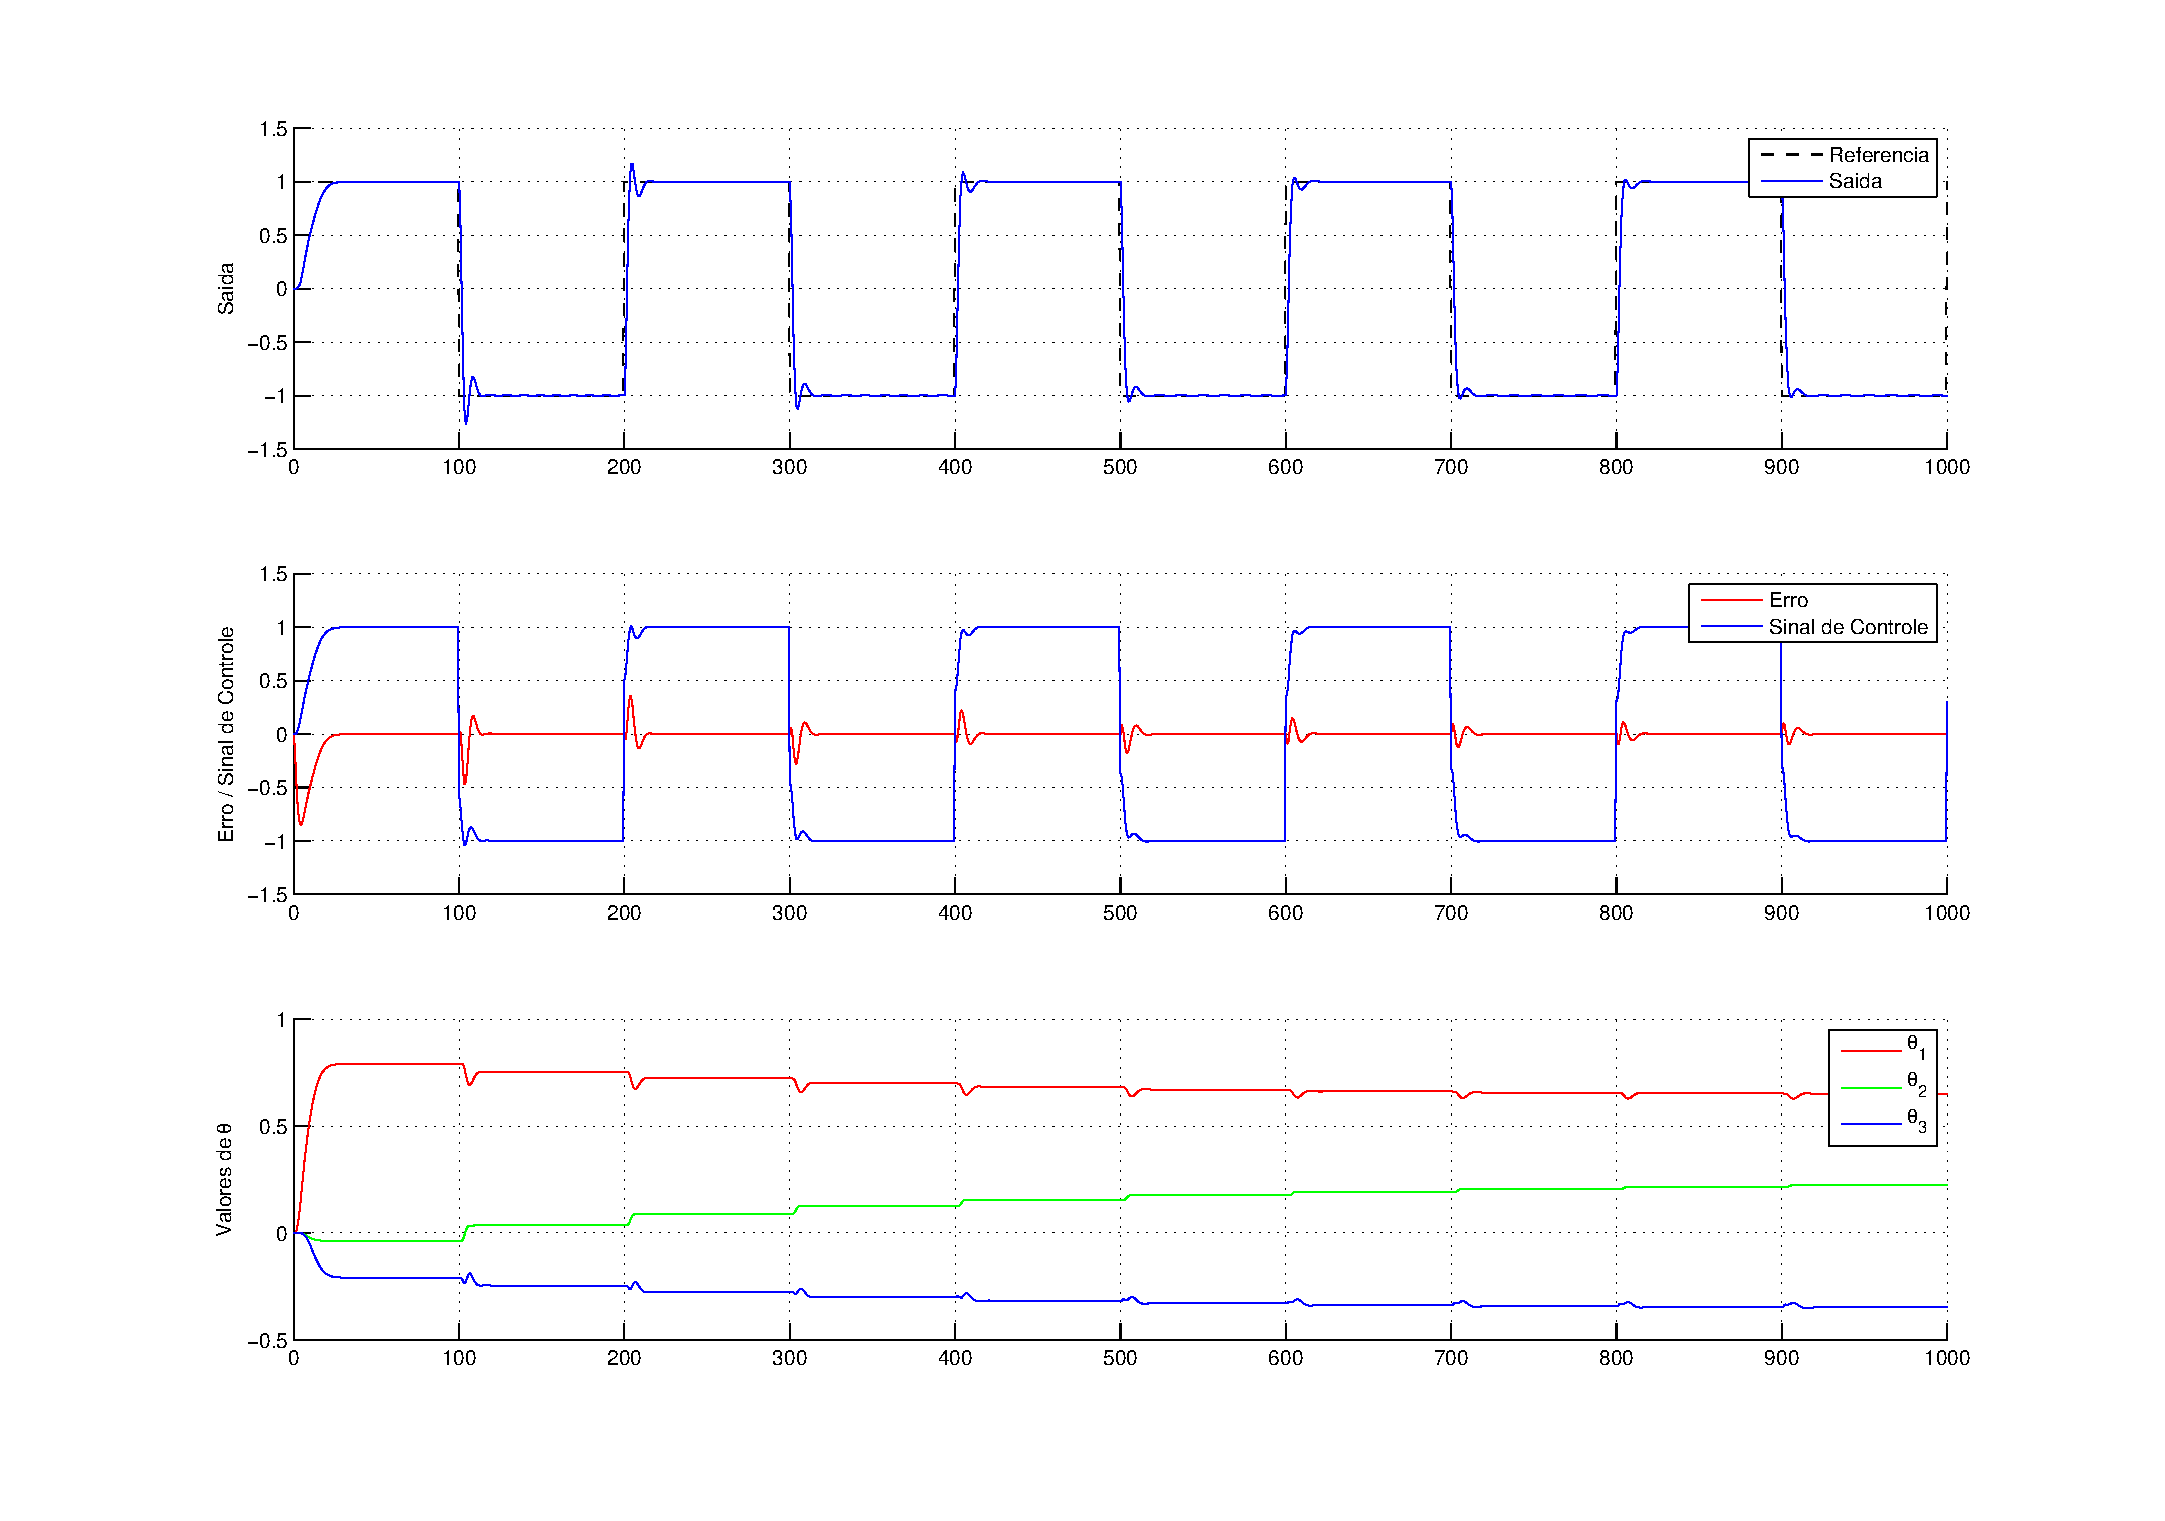
\includegraphics[width=0.95\textwidth]{imgs/questao3/saida_gamma_0.1.eps}
    \caption{Saída do sistema para $\gamma = 0.1$.}
    \label{fig:q3_saida_gamma_0.1}
\end{figure}

\begin{figure}[htb]
    \centering
    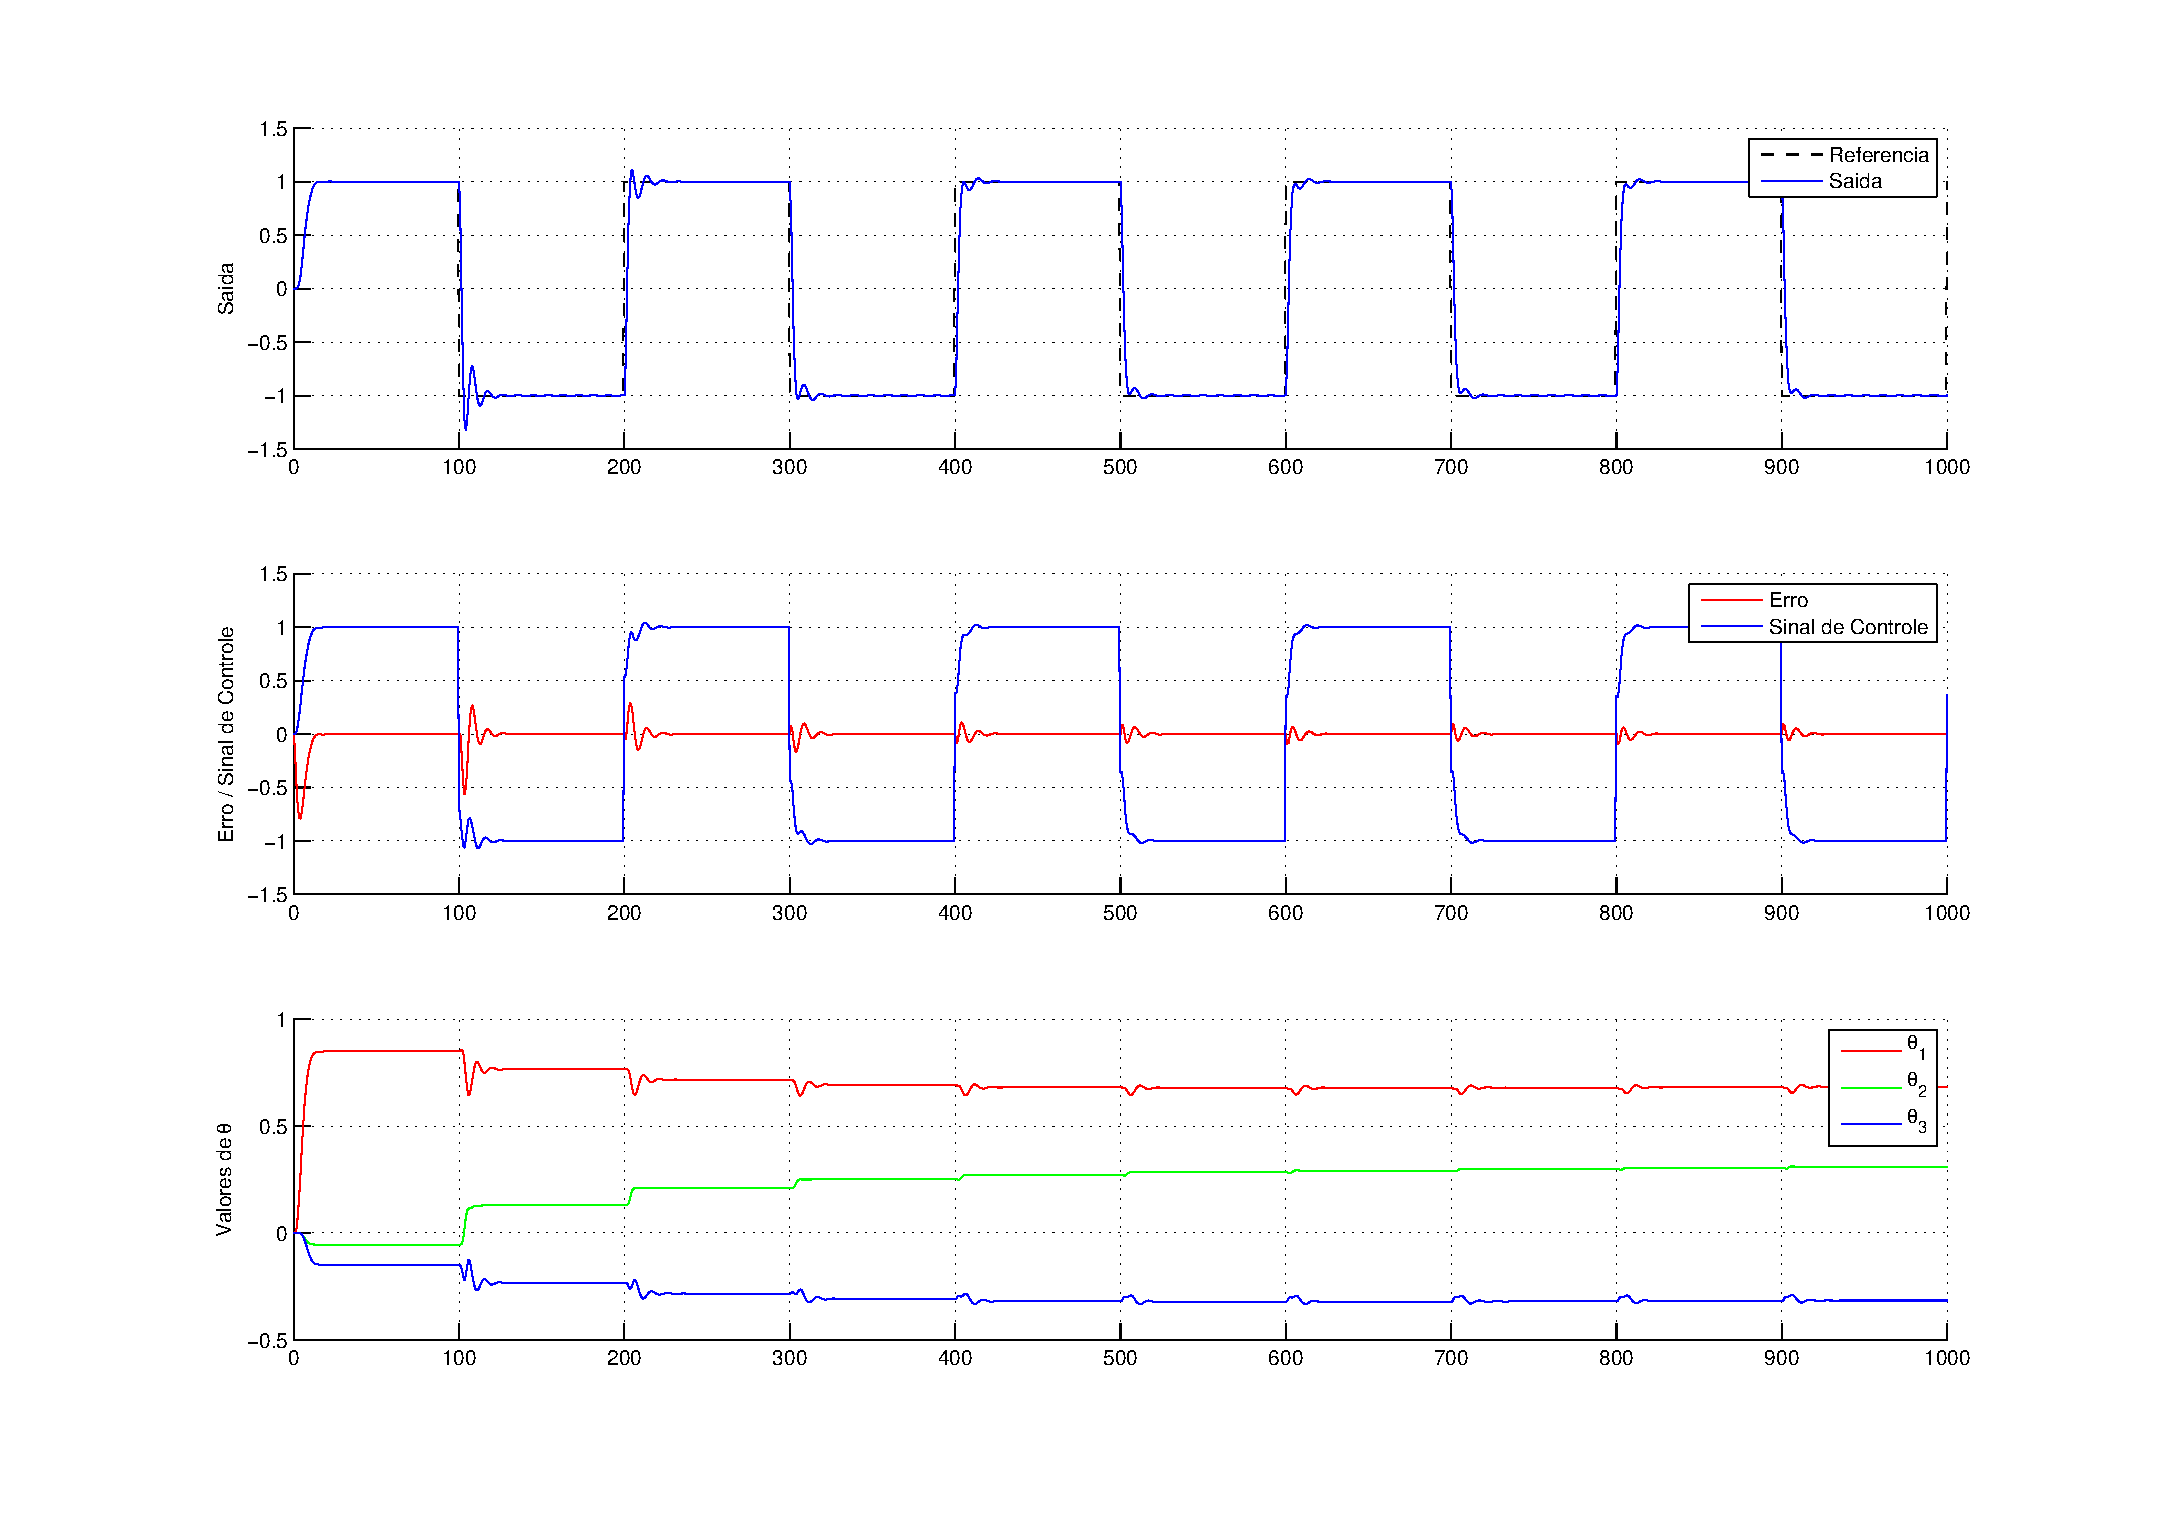
\includegraphics[width=0.95\textwidth]{imgs/questao3/saida_gamma_0.2.eps}
    \caption{Saída do sistema para $\gamma = 0.2$.}
    \label{fig:q3_saida_gamma_0.2}
\end{figure}

\begin{figure}[H]
    \centering
    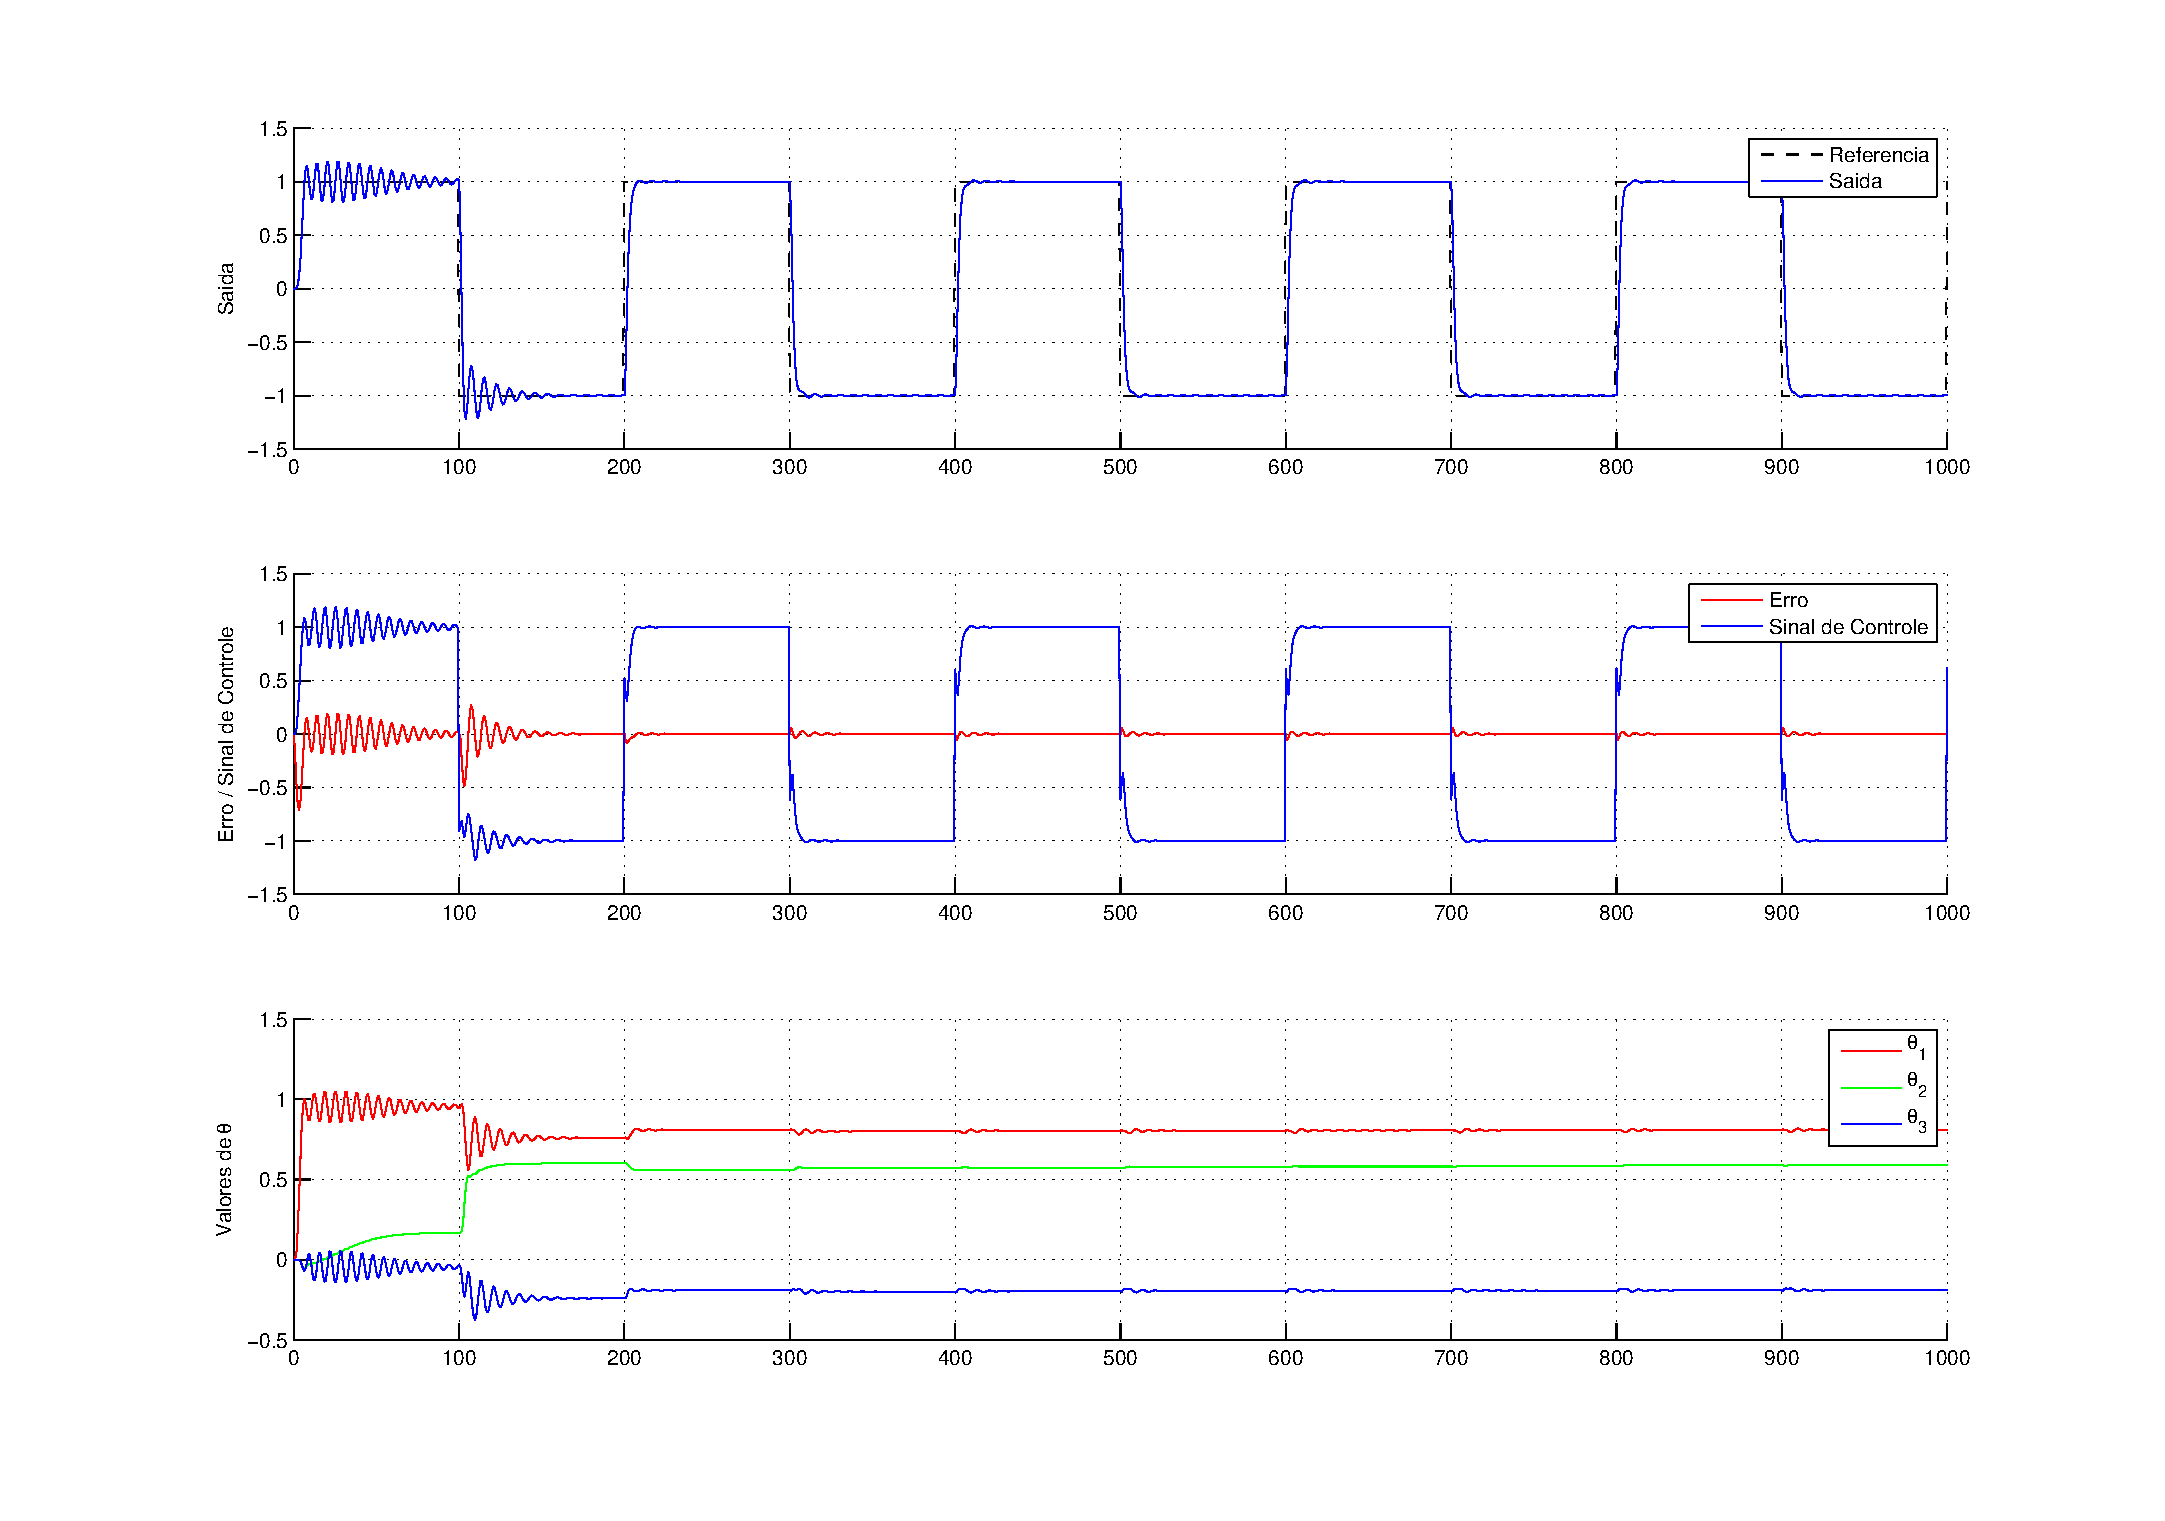
\includegraphics[width=0.95\textwidth]{imgs/questao3/saida_gamma_0.5.eps}
    \caption{Saída do sistema para $\gamma = 0.5$.}
    \label{fig:q3_saida_gamma_0.5}
\end{figure}

\begin{figure}[htb]
    \centering
    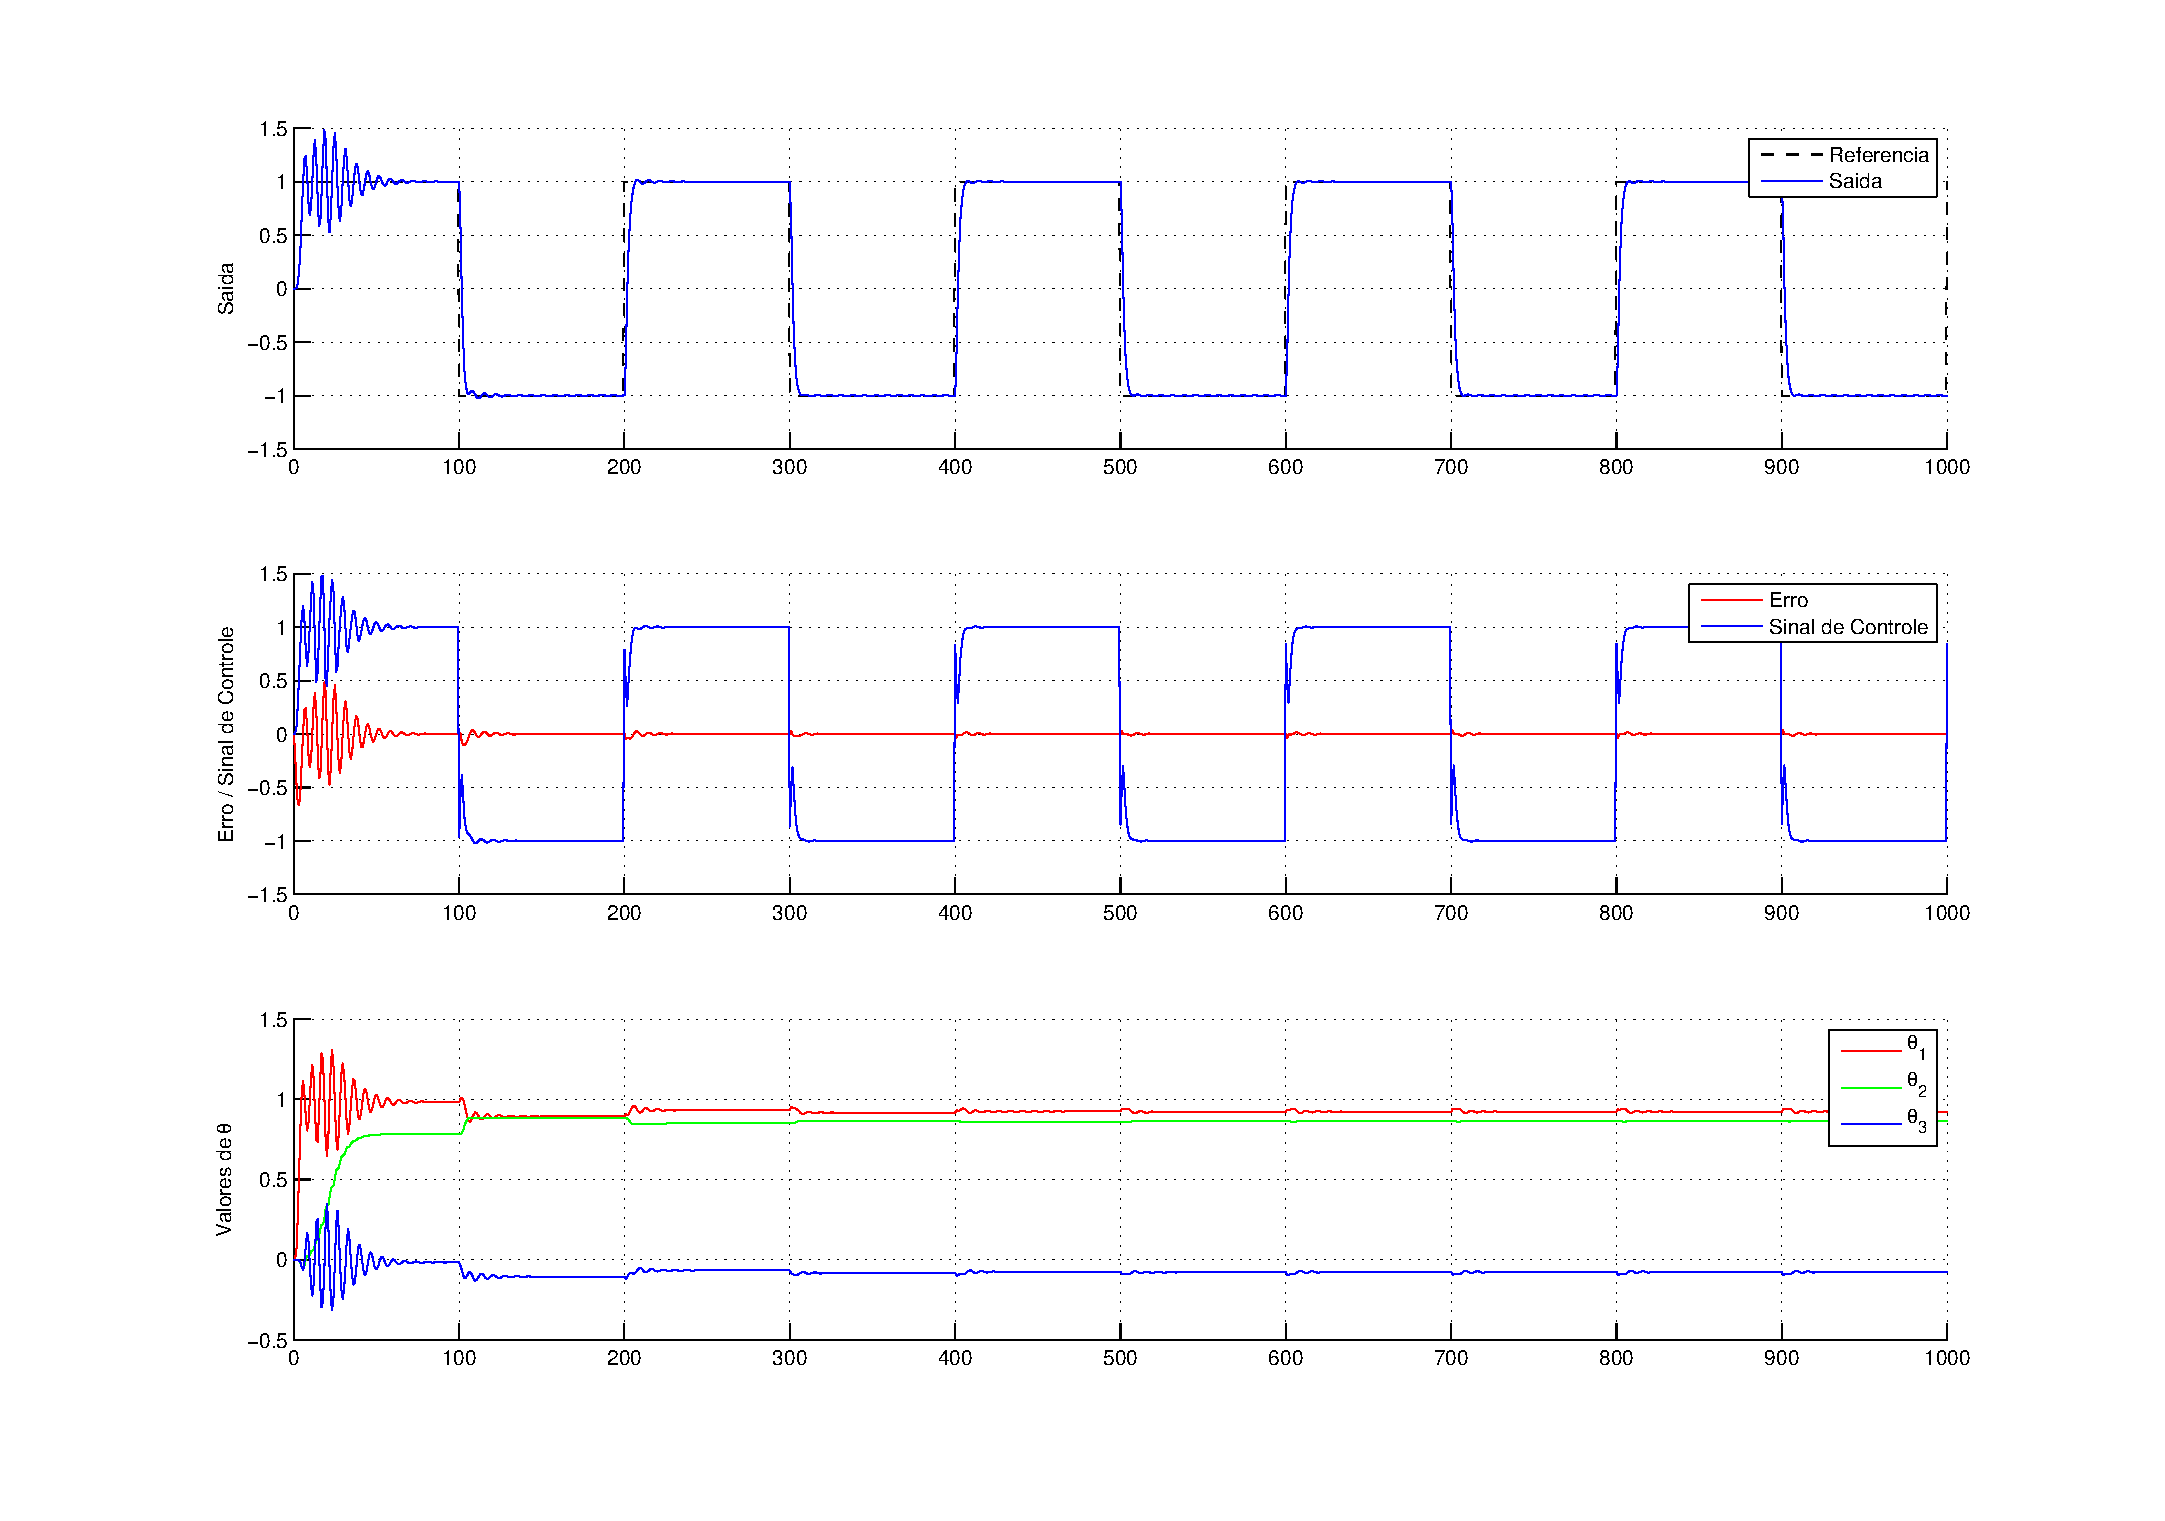
\includegraphics[width=0.95\textwidth]{imgs/questao3/saida_gamma_0.7.eps}
    \caption{Saída do sistema para $\gamma = 0.7$.}
    \label{fig:q3_saida_gamma_0.7}
\end{figure}

\begin{figure}[H]
    \centering
    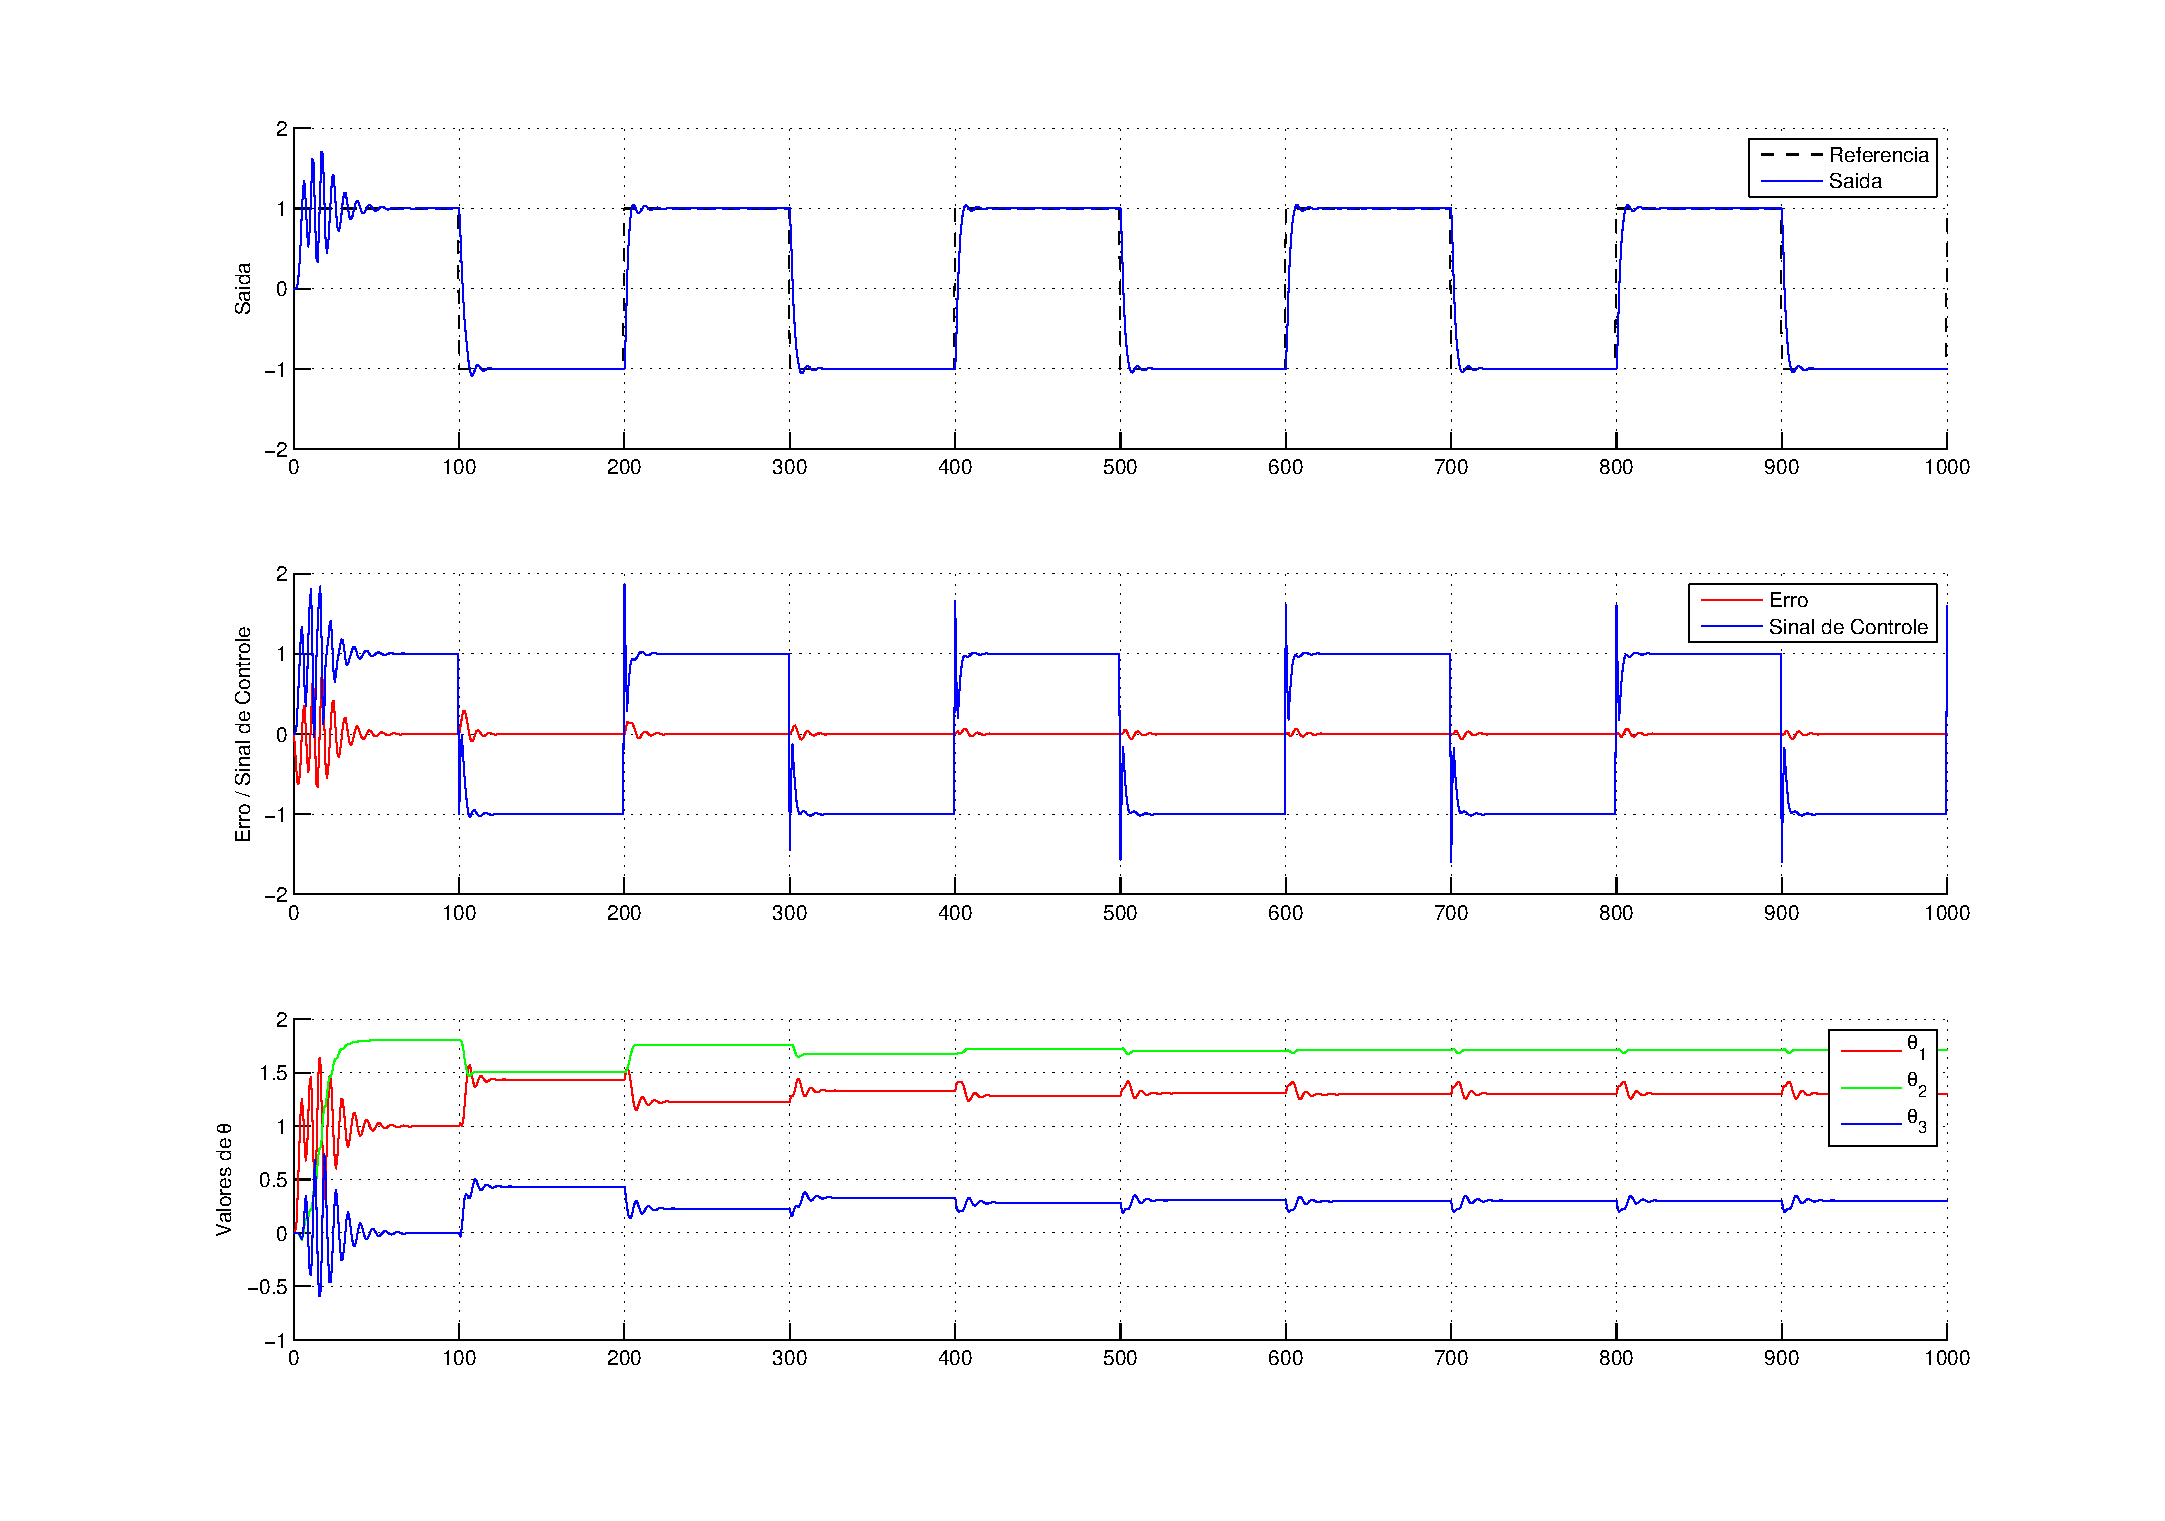
\includegraphics[width=0.95\textwidth]{imgs/questao3/saida_gamma_1.0.eps}
    \caption{Saída do sistema para $\gamma = 1.0$.}
    \label{fig:q3_saida_gamma_1.0}
\end{figure}

Avaliando o desempenho do sistema para os diferentes valores de $\gamma$,
percebe-se que para valores mais altos o sistema possui um sinal de controle
mais agressivo, fazendo com que apareçam oscilações subamortecidas em sua
saída, principalmente com as mudanças de {\it set point}. Por outro lado,
valores pequenos fazem com que a resposta do sistema evolua de maneira suave,
como pode ser comprovado pelos gráficos de $\gamma = 0.1$ e $\gamma = 0.2$.
Entretanto, percebe-se ainda que o erro de seguimento de trajetória é menor para
$\gamma = 0.5$, $\gamma = 0.7$ e $\gamma = 1.0$.

O {\it script} do Matlab\textsuperscript{\textregistered} desenvolvido para a
resolução dessa questão pode ser encontrado no Apêndice \ref{ap:cod_q3}.

\pagebreak
% Universidade Federal do Rio Grande do Norte
% Programa de Pos-Graduacao em Engenharia Eletrica e de Computacao
% Lista 1 - Questao 4
% Autores: Anna Giselle Camara Dantas Ribeiro
%          Cristiano Gurgel de Castro
%          Diogo Leite Reboucas
%          Thiago Medeiros Barros

% Revisado em 15/06/2010 12:38 por crisgc

  \chapter*{Questão 4}
% Enunciado
\noindent {\it Seja o sistema da Fig. \ref{fig:q4:sist}. Considerando $G(s) =
\frac{2e^{-s}}{s+0.25}$, pede-se: }

\begin{itemize}
    \item[a)] {\it projetar um controlador PI de forma que o desempenho do
              sistema em malha fechada não apresente sobre-sinal. Simule a 
              resposta no \Matlab.}
    \item[b)] {\it Considerando o sistema com o controlador projetado no item a
              e considerando $G_d(s) = 1$, projetar um controlador feedforward 
              (realizável) e avaliar o desempenho do sistema completo utilizando
              o \Matlab.}
\end{itemize}

\begin{figure}[H]
\centering
    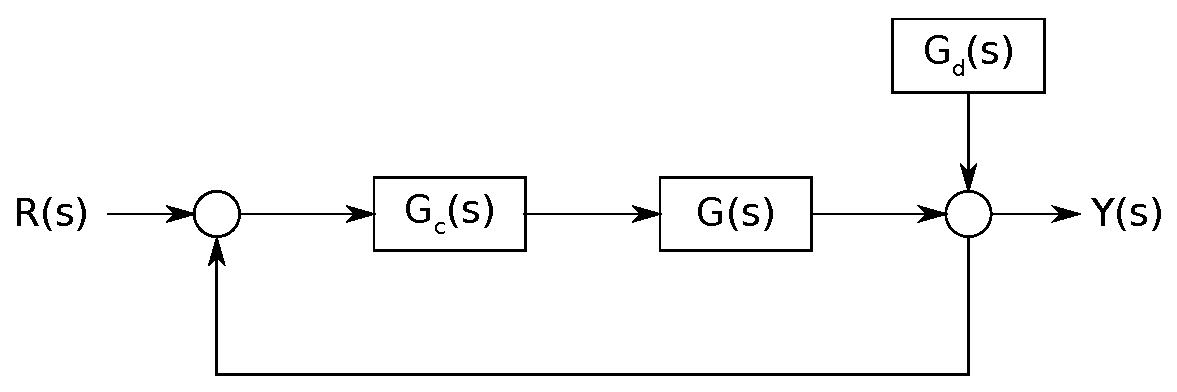
\includegraphics[width=0.65\textwidth]{imgs/questao4/sistema}
    \caption{Diagrama de blocos do sistema.}
    \label{fig:q4:sist}
\end{figure}

% Resolução
\vspace{0.5cm}

\noindent{\bf Resolução:}

\vspace{0.25cm}

% Parte a
O controlador PI foi projetado utilizando o método tradicional, desconsiderando
o atraso do sistema, ou seja, separando o termo $e^{-s}$ do restante da função
de transferência, como pode ser visto na Fig. \ref{fig:q4:projetoPI}.
Definiu-se então $G'(s)$, como sendo a função de transferência sem o atraso de
transporte, ou seja:

\begin{flalign}
G'(s) = \frac{2}{s+0.25} \label{eq:q4:glinha}
\end{flalign}

\begin{figure}[htb]
\centering
\scalebox{0.7}{\begin{picture}(0,0)%
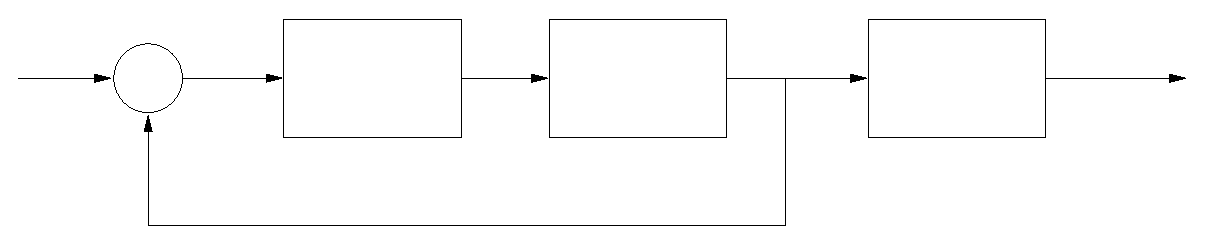
\includegraphics{./imgs/questao4/projetoPI.eps}%
\end{picture}%
\setlength{\unitlength}{4144sp}%
%
\begingroup\makeatletter\ifx\SetFigFont\undefined%
\gdef\SetFigFont#1#2#3#4#5{%
  \reset@font\fontsize{#1}{#2pt}%
  \fontfamily{#3}\fontseries{#4}\fontshape{#5}%
  \selectfont}%
\fi\endgroup%
\begin{picture}(8934,1599)(2914,-3448)
\put(3241,-2176){\makebox(0,0)[b]{\smash{{\SetFigFont{12}{14.4}{\familydefault}{\mddefault}{\updefault}{\color[rgb]{0,0,0}$R(s)$}%
}}}}
\put(5626,-2356){\makebox(0,0)[b]{\smash{{\SetFigFont{12}{14.4}{\familydefault}{\mddefault}{\updefault}{\color[rgb]{0,0,0}$G_c(s)$}%
}}}}
\put(3511,-2536){\makebox(0,0)[b]{\smash{{\SetFigFont{12}{14.4}{\familydefault}{\mddefault}{\updefault}{\color[rgb]{0,0,0}$+$}%
}}}}
\put(4096,-2716){\makebox(0,0)[b]{\smash{{\SetFigFont{12}{14.4}{\familydefault}{\mddefault}{\updefault}{\color[rgb]{0,0,0}$-$}%
}}}}
\put(7651,-2356){\makebox(0,0)[b]{\smash{{\SetFigFont{12}{14.4}{\familydefault}{\mddefault}{\updefault}{\color[rgb]{0,0,0}$\frac{2}{s+0.25}$}%
}}}}
\put(10081,-2356){\makebox(0,0)[b]{\smash{{\SetFigFont{12}{14.4}{\familydefault}{\mddefault}{\updefault}{\color[rgb]{0,0,0}$e^{-s}$}%
}}}}
\put(8911,-2131){\makebox(0,0)[b]{\smash{{\SetFigFont{12}{14.4}{\familydefault}{\mddefault}{\updefault}{\color[rgb]{0,0,0}$Y'(s)$}%
}}}}
\put(11341,-2131){\makebox(0,0)[b]{\smash{{\SetFigFont{12}{14.4}{\familydefault}{\mddefault}{\updefault}{\color[rgb]{0,0,0}$Y(s)$}%
}}}}
\end{picture}%
}
\caption{Projeto de controlador desconsiderando o atraso de transporte.}
\label{fig:q4:projetoPI}
\end{figure}

Primeiramente, analisou-se o sistema em malha fechada sem nenhum controlador ou
seja $G'_c(s) = 1$. O comportamento foi considerado aceitável uma vez que a
saída possui erro de regime aproximadamente nulo e tem uma constante de tempo
razoável (menos de $1$s), conforme Fig.  \ref{fig:q4:saida_mf}. O controlador PI
está, então, adequadamente empregado já que tem por objetivo na sua definição a
melhora do erro de regime.

\begin{figure}[htb]
\centering
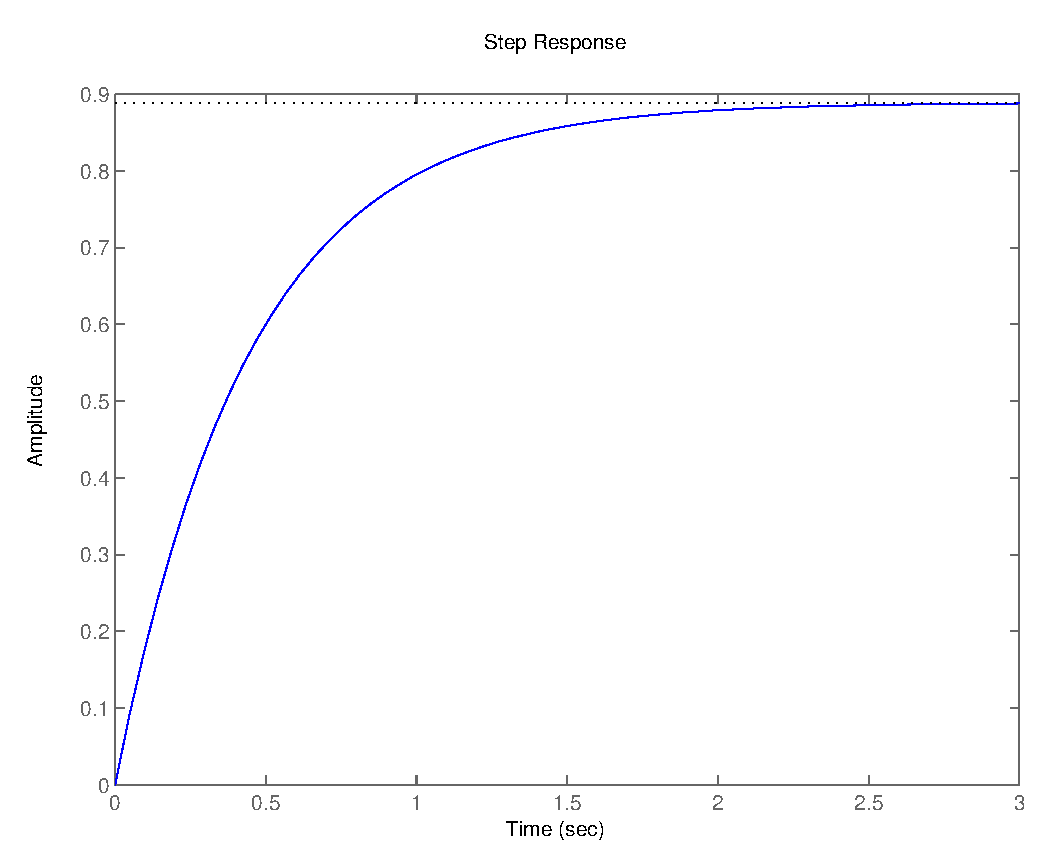
\includegraphics[width=0.65\textwidth]{imgs/questao4/saida_mf}
\caption{Saída do sistema sem o controlador}
\label{fig:q4:saida_mf}
\end{figure}

O requisito do sistema projetado foi a não-presença do sobre-sinal
(\emph{overshoot}). Dessa forma os polos de $G'_c(s)G'(s)$ não devem possuir
parte imaginária, o que significaria oscilações no sinal de saída. Segundo
\citeasnoun{Araujo}, o controlador PI tem a seguinte função de transferência:

\begin{flalign*}
G'_c(s) = k_p + \frac{k_i}{s} = \frac{k_c(s+z)}{s} 
\end{flalign*}

Logo o controlador adiciona um polo na origem e um zero. Para não afetar
demasiadamente as características do transitório, decidiu-se por posicionar o
zero do controlador antes do polo do sistema $G'(s)$, conforme Eq.
\ref{eq:q4:glinha}, ou seja $|z| < 0.25$. O sistema foi simulado com o seguinte
controlador:

\begin{flalign}
G'_c(s) = \frac{s+0.2}{s} \label{eq:q4:glinha_c}
\end{flalign}

\noindent e os resultados obtidos na simulação podem ser visualizados na Fig.
\ref{fig:q4:saida_comp_mf}. O diagrama do lugar geométrico das raízes para o
sistema com o controlador pode ser visualizado na Fig. \ref{fig:q4:rlocus_cmf}.

\begin{figure}[htb]
\centering
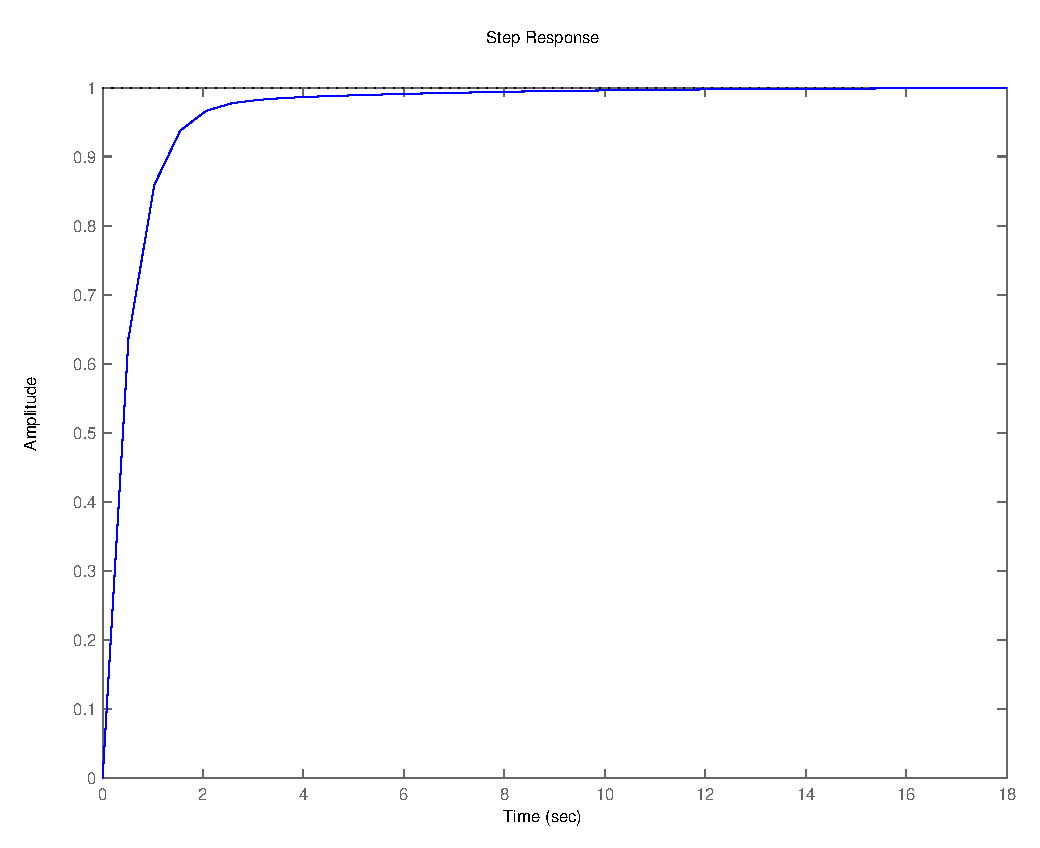
\includegraphics[width=0.65\textwidth]{imgs/questao4/saida_comp_mf}
\caption{Saída do sistema com o controlador projetado $G'_c(s) =
\frac{s+0.2}{s}$.}
\label{fig:q4:saida_comp_mf}
\end{figure}

\begin{figure}[H]
\centering
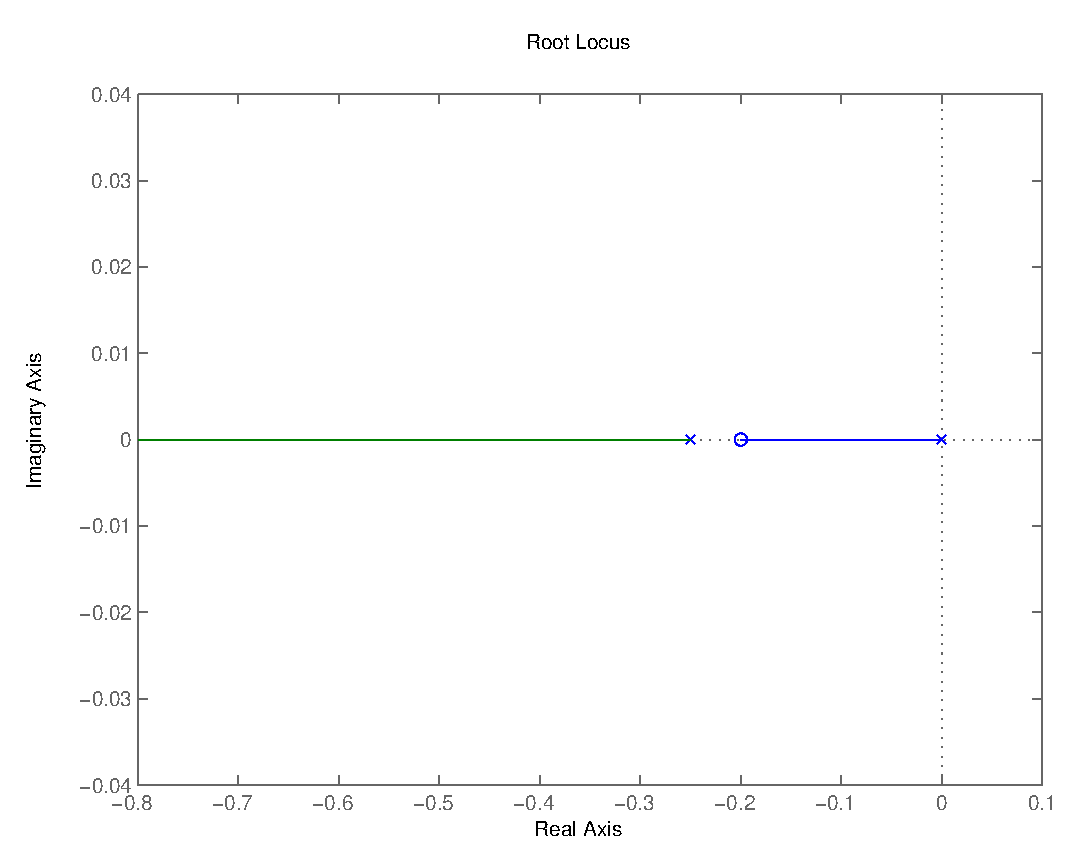
\includegraphics[width=0.65\textwidth]{imgs/questao4/rlocus_cma}
\caption{Lugar das raízes para $G'_c(s)G'(s) = \frac{0.4+2s}{0.25s+s^{2}}$.}
\label{fig:q4:rlocus_cmf}
\end{figure}

A função de transferência de malha fechada para do sistema com o controlador,
juntamente com o valor de $\omega_n$ e $\zeta$ é portanto:

\begin{eqnarray}
G'_{\text{MF}}(s) = \frac{G'_c(s)G'(s)}{1+G'_c(s)G'(s)} =
                    \frac{0.4+2s}{0.4+2.25s+s^{2}}
\end{eqnarray}

\noindent tal que $\omega_n \approx 0.632$ e $\zeta \approx 1.779$.

De acordo com \citeasnoun{Medeiros}, percebe-se que o sistema é sobreamortecido,
já que $\zeta > 1$, portanto a resposta não apresenta o sobressinal. Simulou-se
através do \Simulink\ o desempenho do compensador PI projetado no controle
do sistema $G(s)$ original, ou seja, com o atraso de transporte. O desempenho
foi completamente insatisfatório: o sistema tornou-se instável, conforme Fig.
\ref{fig:q4:saida_cont_dt}. 

\begin{figure}[htb]
\centering
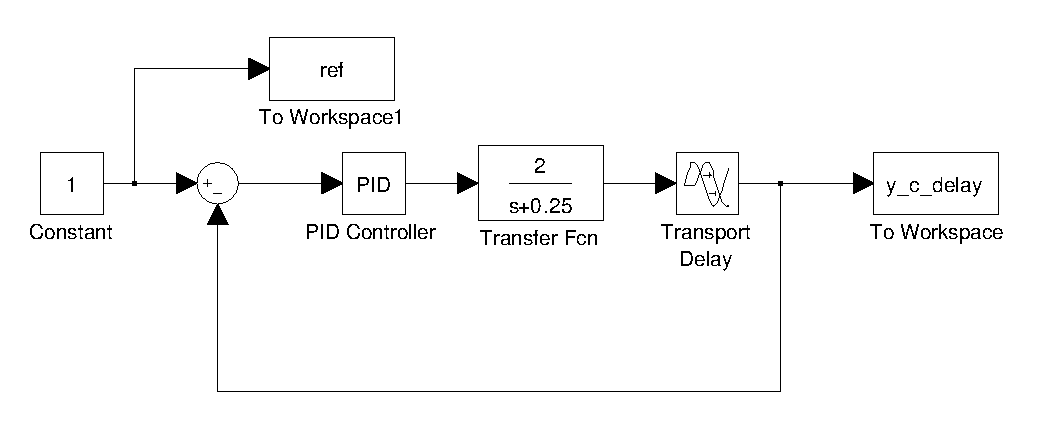
\includegraphics[width=0.65\textwidth]{imgs/questao4/sist_cont_dt}
\caption{Sistema com atraso controlado pelo PI.}
\label{fig:q4:sist_cont_dt}
\end{figure}

\begin{figure}[htb]
\centering
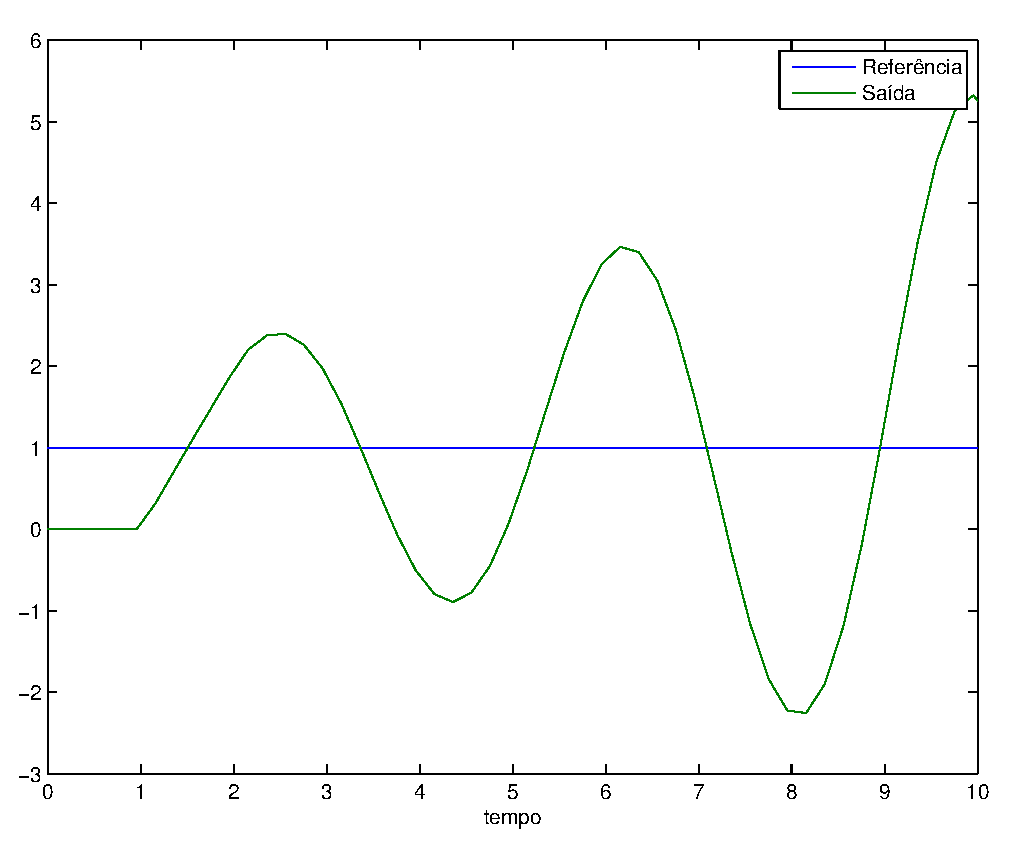
\includegraphics[width=0.65\textwidth]{imgs/questao4/saida_cont_dt}
\caption{Resposta do sistema da Fig. \ref{fig:q4:sist_cont_dt}.}
\label{fig:q4:saida_cont_dt}
\end{figure}

Foi adotado então o preditor de Smith, o qual implementa um tipo de predição
baseado no modelo e possibilita ao controlador projetado agir baseado na
predição $y'(t + L)$, onde $L$ é o atraso de transporte, ou seja, permite ao
controlador agir no sistema como se não houvesse atraso de transporte
\cite{Haegglund1996}. \citeasnoun{Haegglund1996} também justifica porque o tipo
de controlador normalmente usado com preditor de Smith é o PI. O sistema
utilizado para a implementação do preditor bem como o resultado obtido são
mostrados nas Figs. \ref{fig:q4:sist_smith} e \ref{fig:q4:saida_smith}. É
importante ressaltar que nesse preditor foi utilizada uma função de
transferência para predição $\hat{G}(s) = \frac{2}{s+0.25}$ igual, portanto, ao
sistema sem o atraso.

\begin{figure}[htb]
\centering
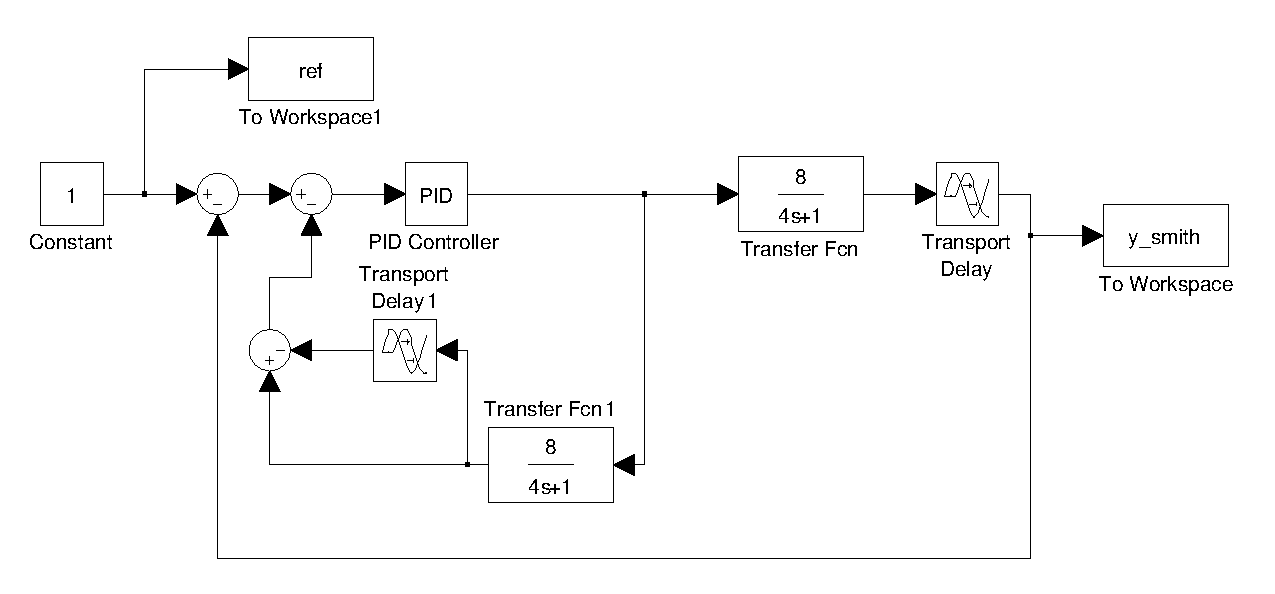
\includegraphics[width=0.75\textwidth]{imgs/questao4/sist_smith}
\caption{Preditor de Smith.}
\label{fig:q4:sist_smith}
\end{figure}

\begin{figure}[htb]
\centering
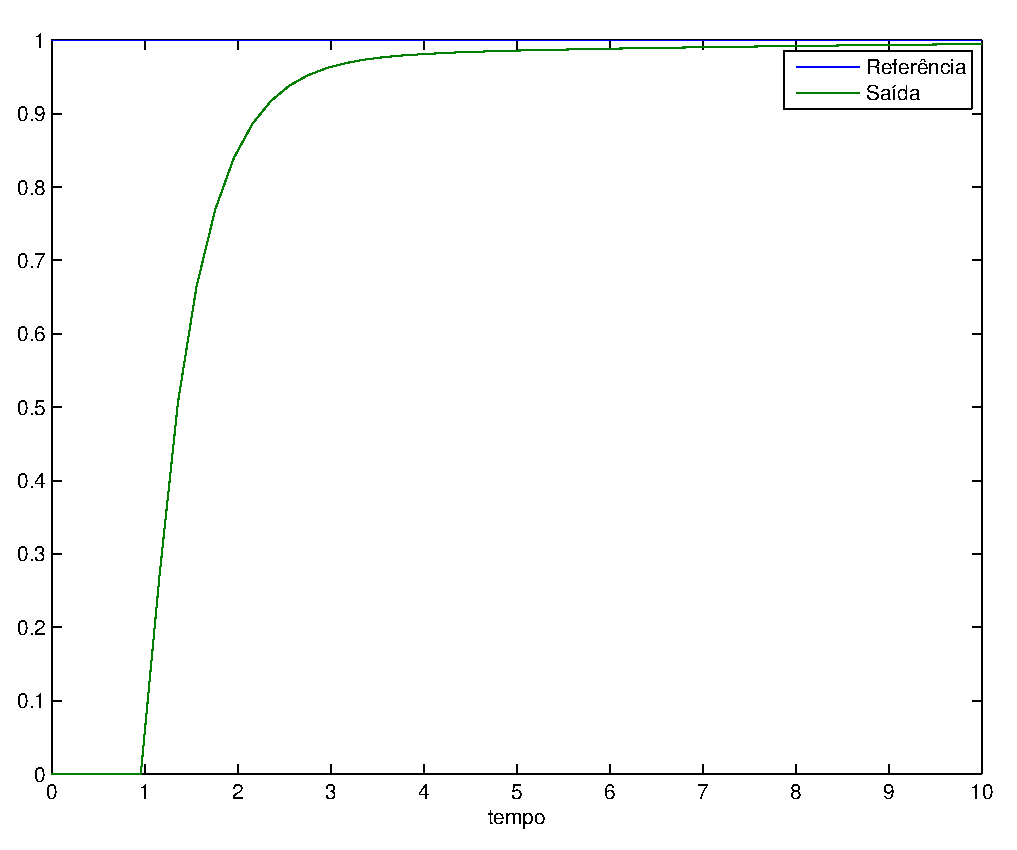
\includegraphics[width=0.65\textwidth]{imgs/questao4/saida_smith}
\caption{Resposta ao controlador com preditor da Fig. \ref{fig:q4:sist_smith}.}
\label{fig:q4:saida_smith}
\end{figure}

Foi analisado também o comportamento do preditor quando o sistema utilizado para
predição não corresponde exatamente ao processo simulado ou seja $\hat{G}(s)
\neq G'(s)$, conforme Fig. \ref{fig:q4:sist_smith_diff}. Apesar de ter
apresentado um baixo e indesejável sobressinal, o resultado foi razoável,
conforme Fig. \ref{fig:q4:saida_smith_diff}, o que mostra a boa adequação do
preditor mesmo com estimativas grosseiras da função de transferência do sistema
original. Escolheu-se para a continuação da questão o sistema tal que
$\hat{G}(s) = G'(s)$. A função de transferência final do controlador é,
portanto: 

\begin{flalign}
G_c(s) = \frac{G'_c(s)}{1 + G'_c(s)(1 - e^{-s})\hat{G}(s)} =
\frac{G'_c(s)}{1 + G'_c(s)(1 - e^{-s})G'(s)} \label{eq:q4:g_c}
\end{flalign}

\begin{figure}[htb]
\centering
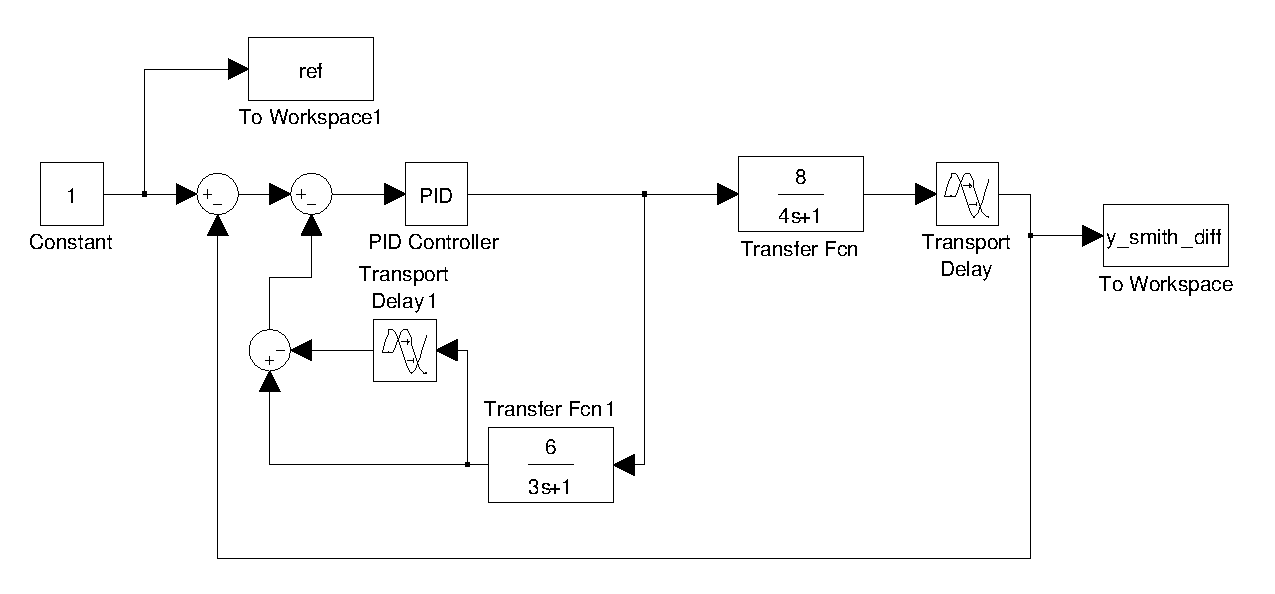
\includegraphics[width=0.65\textwidth]{imgs/questao4/sist_smith_diff}
\caption{Preditor de Smith com $G'(s) = \frac{6}{3s + 1}$.}
\label{fig:q4:sist_smith_diff}
\end{figure}

\begin{figure}[htb]
\centering
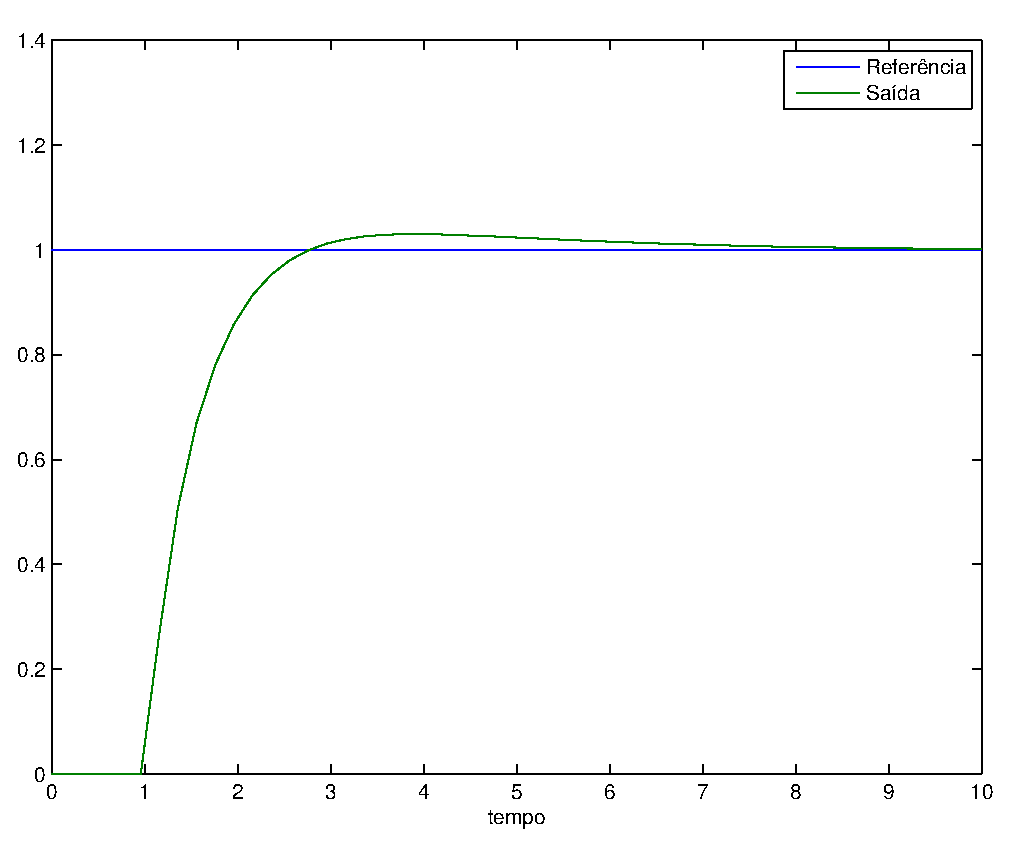
\includegraphics[width=0.65\textwidth]{imgs/questao4/saida_smith_diff}
\caption{Resposta ao controlador com preditor da Fig.
\ref{fig:q4:sist_smith_diff}.}
\label{fig:q4:saida_smith_diff}
\end{figure}

% Parte b

% Considerações sobre Gff(s)
Projetado o controlador PI, analisou-se então o acréscimo do controle {\it
feedforward} ($G_\text{ff}(s)$) ao processo, conforme Fig. \ref{fig:q4:sist_ff}.
Através da análise da figura, com o intuito de cancelar efeito do ruído, tem-se
que:

\begin{flalign*}
G'_\text{ff}(s) & = \frac{G_d(s)}{\underbrace{G_c(s)}_{\text{Eq.
\ref{eq:q4:g_c}}}G(s)} = \frac{1 + G'(s)G'_c(s) -
e^{-s}G'(s)G'_c(s)}{G'(s)G'_c(s)e^{-s}} \\
& = \frac{1 + G'(s)G'_c(s)}{G'(s)G'_c(s)}e^{s} - 1
\end{flalign*}

A partir de $G'_\text{ff}(s)$, pode-se notar que o compensador ideal é irrealizável,
já que envolve tanto um retorno no tempo $e^{s}$, quanto um impulso unitário $1$. Isso
poderia ser previamente notado, sem nenhum cálculo de função de transferência,
através da análise de duas características do sistema:

\begin{itemize}
\item o distúrbio ($D(s)$) atua no sistema instantaneamente, já que $G_d(s) =
1$;
\item qualquer ação na variável manipulada do sistema demorará um tempo $\tau =
1$ para ser refletida na saída, onde $\tau$ é o chamado atraso de transporte do sistema.
\end{itemize}

\begin{figure}[htb]
\centering
\scalebox{0.7}{\begin{picture}(0,0)%
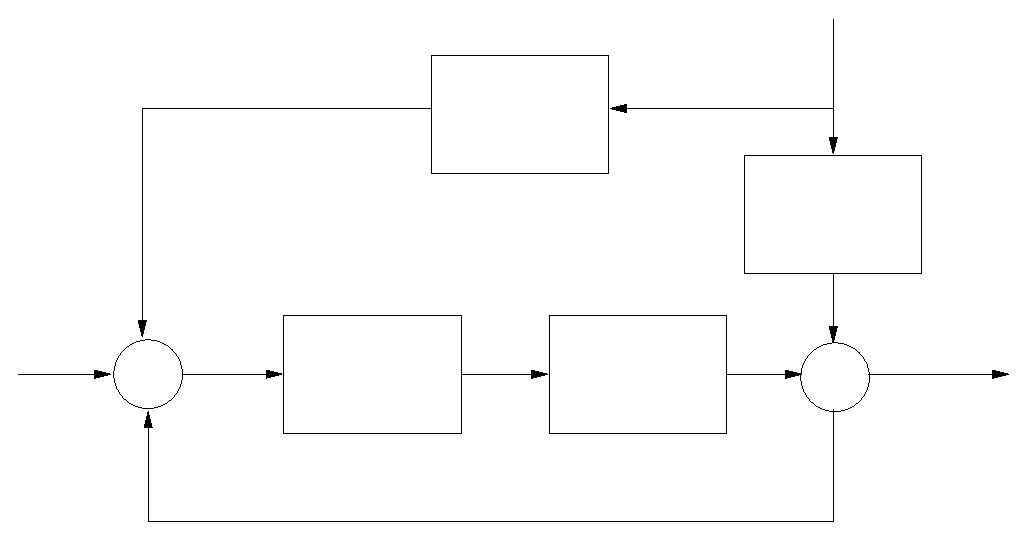
\includegraphics{./imgs/questao4/sist_ff.eps}%
\end{picture}%
\setlength{\unitlength}{4144sp}%
%
\begingroup\makeatletter\ifx\SetFigFont\undefined%
\gdef\SetFigFont#1#2#3#4#5{%
  \reset@font\fontsize{#1}{#2pt}%
  \fontfamily{#3}\fontseries{#4}\fontshape{#5}%
  \selectfont}%
\fi\endgroup%
\begin{picture}(7584,3849)(2914,-3448)
\put(3241,-2176){\makebox(0,0)[b]{\smash{{\SetFigFont{12}{14.4}{\familydefault}{\mddefault}{\updefault}{\color[rgb]{0,0,0}$R(s)$}%
}}}}
\put(5626,-2356){\makebox(0,0)[b]{\smash{{\SetFigFont{12}{14.4}{\familydefault}{\mddefault}{\updefault}{\color[rgb]{0,0,0}$G_c(s)$}%
}}}}
\put(3511,-2536){\makebox(0,0)[b]{\smash{{\SetFigFont{12}{14.4}{\familydefault}{\mddefault}{\updefault}{\color[rgb]{0,0,0}$+$}%
}}}}
\put(4096,-2716){\makebox(0,0)[b]{\smash{{\SetFigFont{12}{14.4}{\familydefault}{\mddefault}{\updefault}{\color[rgb]{0,0,0}$-$}%
}}}}
\put(7651,-2356){\makebox(0,0)[b]{\smash{{\SetFigFont{12}{14.4}{\familydefault}{\mddefault}{\updefault}{\color[rgb]{0,0,0}$G(s)$}%
}}}}
\put(9136,-1141){\makebox(0,0)[b]{\smash{{\SetFigFont{12}{14.4}{\familydefault}{\mddefault}{\updefault}{\color[rgb]{0,0,0}$G_d(s)$}%
}}}}
\put(6751,-331){\makebox(0,0)[b]{\smash{{\SetFigFont{12}{14.4}{\familydefault}{\mddefault}{\updefault}{\color[rgb]{0,0,0}$G_{ff}(s)$}%
}}}}
\put(8686,-2491){\makebox(0,0)[b]{\smash{{\SetFigFont{12}{14.4}{\familydefault}{\mddefault}{\updefault}{\color[rgb]{0,0,0}$+$}%
}}}}
\put(9361,-1996){\makebox(0,0)[b]{\smash{{\SetFigFont{12}{14.4}{\familydefault}{\mddefault}{\updefault}{\color[rgb]{0,0,0}$+$}%
}}}}
\put(4051,-1951){\makebox(0,0)[b]{\smash{{\SetFigFont{12}{14.4}{\familydefault}{\mddefault}{\updefault}{\color[rgb]{0,0,0}$-$}%
}}}}
\put(10081,-2131){\makebox(0,0)[b]{\smash{{\SetFigFont{12}{14.4}{\familydefault}{\mddefault}{\updefault}{\color[rgb]{0,0,0}$Y(s)$}%
}}}}
\put(9586,-16){\makebox(0,0)[b]{\smash{{\SetFigFont{12}{14.4}{\familydefault}{\mddefault}{\updefault}{\color[rgb]{0,0,0}$D(s)$}%
}}}}
\end{picture}%
}
\caption{Projeto de controlador desconsiderando o atraso de transporte.}
\label{fig:q4:sist_ff}
\end{figure}

Com isso, qualquer ruído detectado em um determinado momento, somente poderá a ser
compensado após o atraso de transporte do sistema, portanto o cancelamento de ruído
perfeito não é possível, o que se reflete em um $G'_\text{ff}(s)$ irrealizável. 

% Realizando G_ff
A partir do modelo ideal $G'_\text{ff}(s)$, $G_\text{ff}(s)$ foi projetado eliminando-se o
termo $e^{s}$, assim sendo:

\begin{flalign*}
G_\text{ff}(s) & = \frac{1 + G'(s)G'_c(s)}{G'(s)G'_c(s)}\cancel{e^{s}} - 1 =
\frac{1}{\underbrace{G'(s)}_{\text{Eq.
\ref{eq:q4:glinha}}}\underbrace{G'_c(s)}_{\text{Eq. \ref{eq:q4:glinha_c}}}}
\cancel{+ 1 - 1} = \frac{s(s+0.25)}{2(s+0.2)} \\
& = \frac{1}{2}\frac{s^2 + 0.25s}{s + 0.2}
\end{flalign*}

Observa-se que o número de zeros supera o de polos no sistema. Para contornar o
problema adicionou-se em série dois filtros (passa-baixa) na equação de
transferência $G_\text{ff}(s)$, foram testados dois tipos de filtros $F_1(s) =
\frac{1}{s+1}$ e $F_{10}(s) = \frac{10}{s+10}$, esses filtros possuem ganho
estático $1$ e não influenciam o regime do sistema. 

Analisou-se o comportamento da resposta de três sistemas. O primeiro deles sem o
controle {\it feedforward}, cujos resultados podem ser observados na Fig.
\ref{fig:q4:sist_ruido}.

O segundo dado pela função de transferência $G_{\text{ff}_1}(s)$ apresentada na
Eq. \ref{eq:q4:g_ff1}, cujos resultados podem ser observados na Fig.
\ref{fig:q4:sist_ruido_ff1}.

\begin{flalign}
F_1(s) & = \frac{1}{s+1} \nonumber \\
G_{\text{ff}_1} & = G_\text{ff}(s)F_1(s)F_1(s) = \frac{1}{2}\frac{s^2 + 0.25s}{s +
0.2}\frac{1}{s+1}\frac{1}{s+1} = 0.5\frac{0.25s+s^{2}}{0.2+1.4s+2.2s^{2}+s^{3}}
\label{eq:q4:g_ff1}
\end{flalign}

Por fim, o terceiro dado pela função de transferência $G_{\text{ff}_{10}}(s)$
apresentada na Eq. \ref{eq:q4:g_ff10}, cujos resultados podem ser observados na
Fig. \ref{fig:q4:sist_ruido_ff10}. 

\begin{flalign}
F_{10}(s) & = \frac{10}{s+10} \nonumber \\
G_{\text{ff}_{10}} & = G_\text{ff}(s)F_{10}(s)F_{10}(s) = 
                       \frac{1}{2}\frac{s^2 + 0.25s}{s +0.2}\frac{10}{s+10}
                       \frac{10}{s+10} = 50\frac{s^{2}+0.25s}
                                                {s^{3}+20.2s^{2}+104s+20}
\label{eq:q4:g_ff10}
\end{flalign}

O tipo de ruído utilizado foi um sinal tipo degrau unitário agindo a partir de
$t_r = 5$. Os resultados para os três sistemas estão apresentados nas Figs.
\ref{fig:q4:saida_ruido}, \ref{fig:q4:saida_ruido_ff1} e
\ref{fig:q4:saida_ruido_ff10}, respectivamente.

\begin{figure}[htb]
\centering
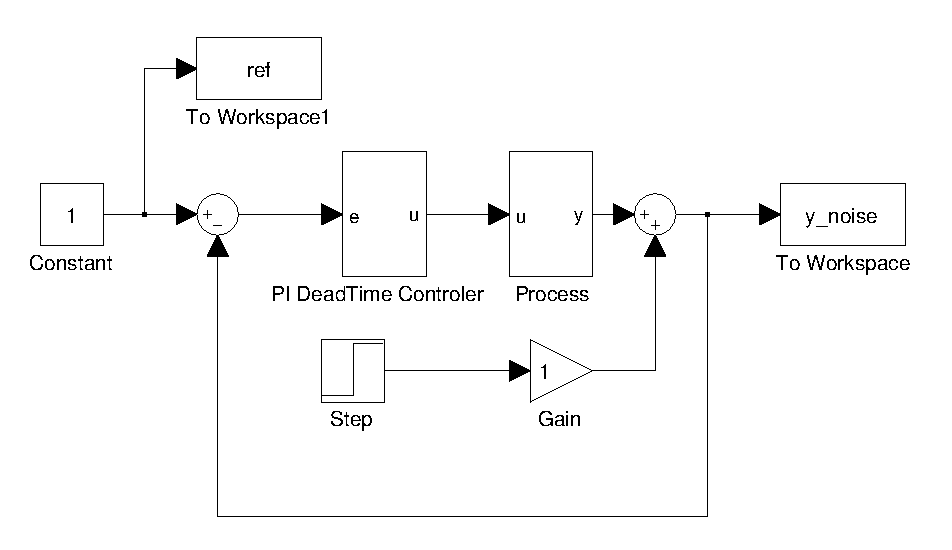
\includegraphics[width=0.75\textwidth]{imgs/questao4/sist_ruido}
\caption{Sistema com ruído na saída sem compensação {\it feedforward}.}
\label{fig:q4:sist_ruido}
\end{figure}

\begin{figure}[htb]
\centering
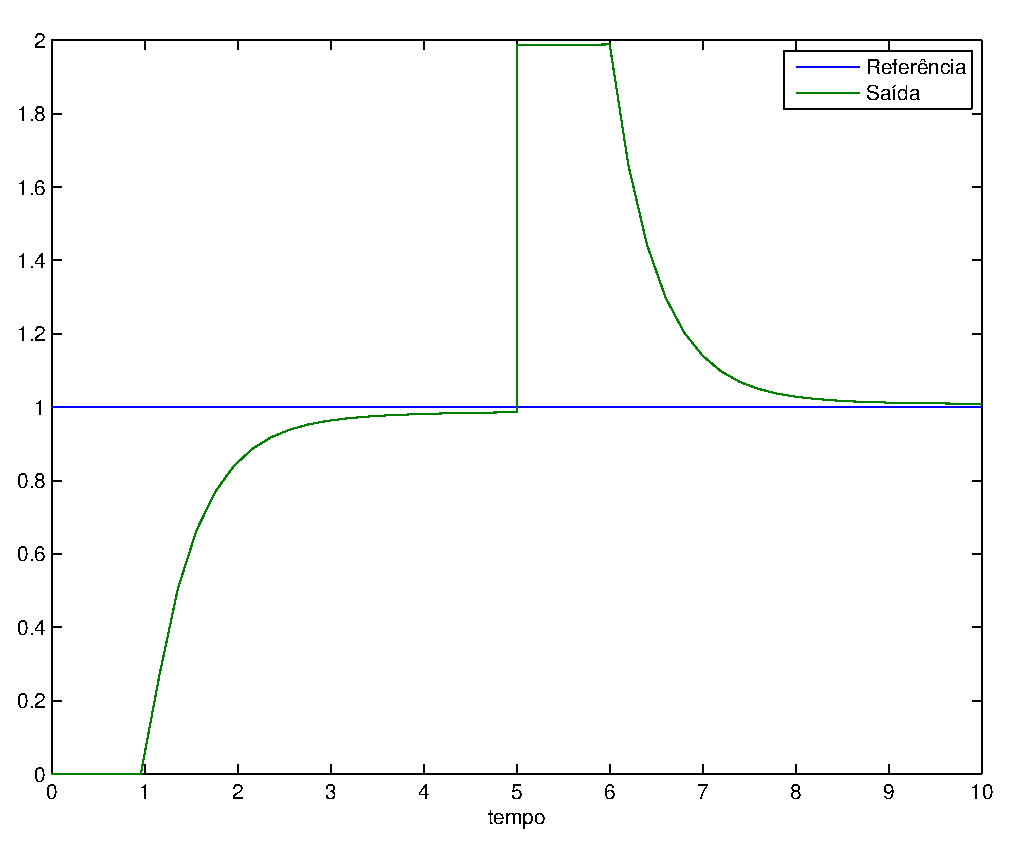
\includegraphics[width=0.65\textwidth]{imgs/questao4/saida_ruido}
\caption{Resposta do sistema da Fig. \ref{fig:q4:sist_ruido}.}
\label{fig:q4:saida_ruido}
\end{figure}

\begin{figure}[htb]
\centering
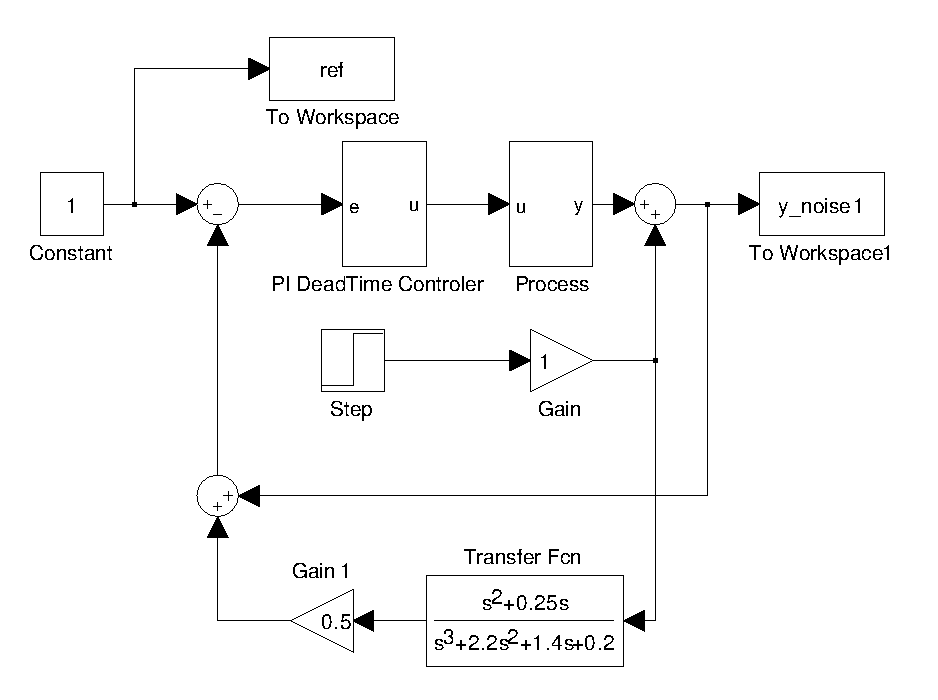
\includegraphics[width=0.75\textwidth]{imgs/questao4/sist_ruido_ff1}
\caption{Sistema com ruído na saída com compensação {\it feedforward} 
         $G_{\text{ff}_1}$.}
\label{fig:q4:sist_ruido_ff1}
\end{figure}

\begin{figure}[H]
\centering
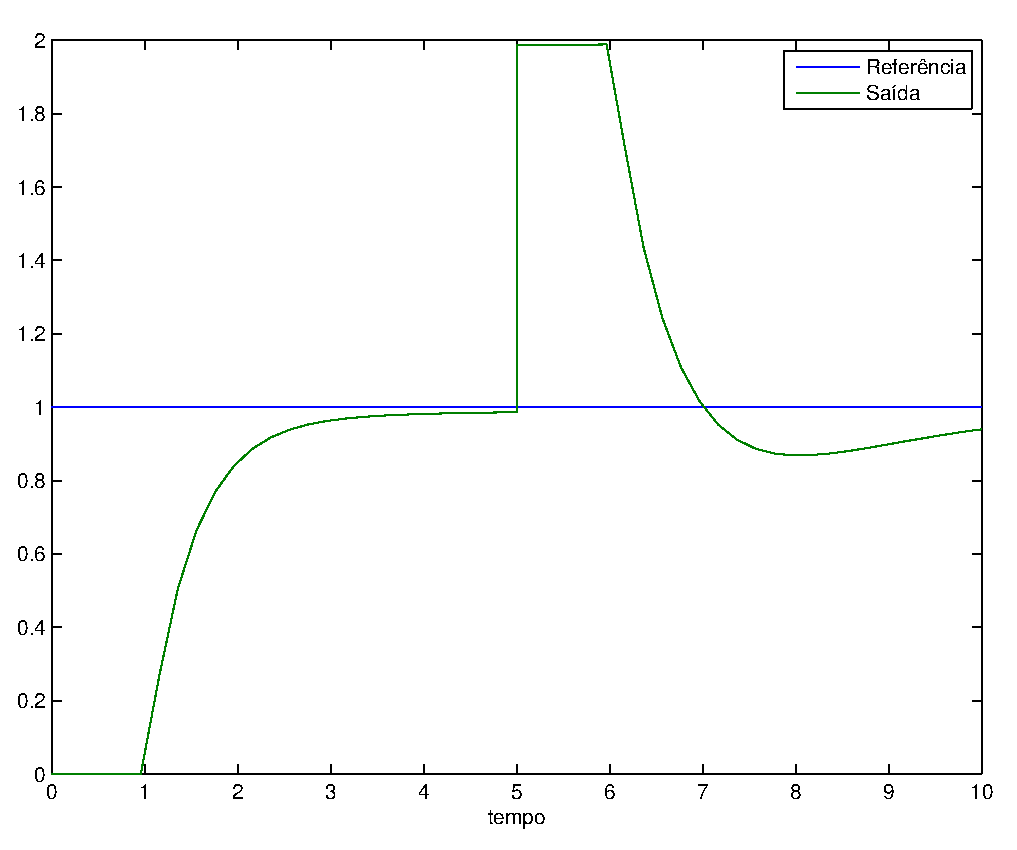
\includegraphics[width=0.65\textwidth]{imgs/questao4/saida_ruido_ff1}
\caption{Resposta do sistema da Fig. \ref{fig:q4:sist_ruido_ff1}.}
\label{fig:q4:saida_ruido_ff1}
\end{figure}

\begin{figure}[H]
\centering
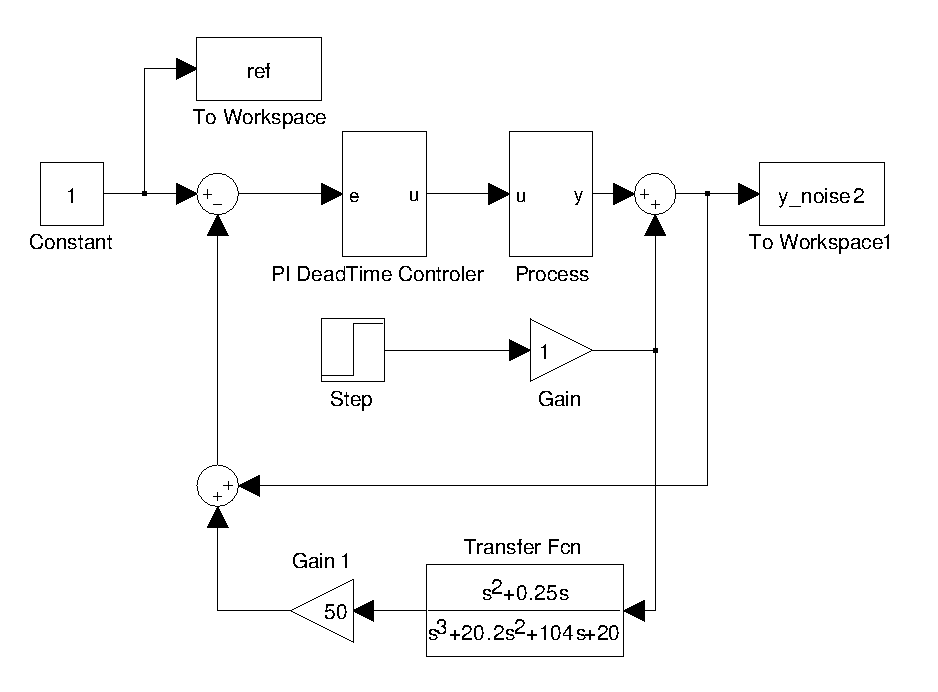
\includegraphics[width=0.75\textwidth]{imgs/questao4/sist_ruido_ff2}
\caption{Sistema com ruido na saída com compensação {\it feedforward}
         $G_{\text{ff}_{10}}$}
\label{fig:q4:sist_ruido_ff10}
\end{figure}

\begin{figure}[H]
\centering
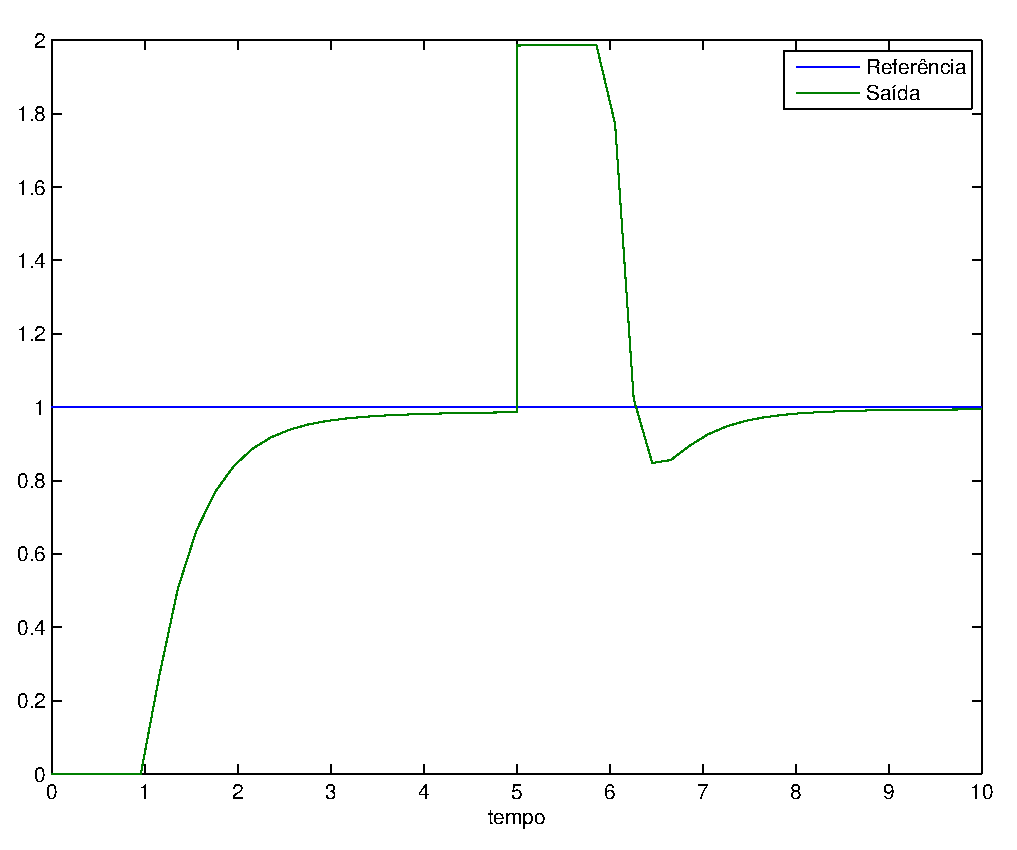
\includegraphics[width=0.65\textwidth]{imgs/questao4/saida_ruido_ff2}
\caption{Resposta do sistema da Fig. \ref{fig:q4:sist_ruido_ff10}.}
\label{fig:q4:saida_ruido_ff10}
\end{figure}

Observando-se o resultado dos três sistemas nota-se que, nesse caso, apesar do
que o próprio nome sugere, o controle {\it feedforward}, não irá atuar
antecipadamente em relação ao controle PI já instalado, pois, já que o distúrbio
atua instantaneamente na saída, o sinal de erro por ele gerado é detectado
(também instantaneamente) pelo controlador PI (com preditor) já instalado. Por
essa razão o sinal de saída do sistema sem o controle FF não se diferencia muito
em termos de desempenho dos sistemas com controle {\it feedforward}.

No entanto a adiçãoda compensação FF, possui uma diferença básica, a rapidez da
reação ao ruído após o tempo $t_r + \tau$, ou seja, passado o intervalo do
atraso de transporte após a aplicação do ruído, como pode ser visto na Fig.
\ref{fig:q4:saida_ruido_ff10}, na qual há um sobressinal na compensação do
ruído. Esse comportamento é devido à excitação do controlador $G_c(s)$ não
somente pelo erro gerado pelo ruído mas também sinal proveniente de
$G_\text{ff}(s)$ e possui a característica de causar um sobressinal no
restabelecimento da referência. A reação ao ruído na Fig.
\ref{fig:q4:sist_ruido_ff1}, no entanto, é bastante lenta, devido aos dois
filtros $F_1(s)$ utilizados, por possuírem uma constante de tempo elevada
($1$), apresentando o pior desempenho entre os três.

\pagebreak
\appendix
\chapter{\bf Código da Questão 1}\label{ap:cod_q1}

%\lstset{language=matlab,
%        numbers=left,
%        basicstyle=\scriptsize,
%        stepnumber=2,
%        numbersep=10pt,
%        showspaces=false,
%        showtabs=false,
%        showstringspaces=false,
%        morecomment=[l]{\%}
%        }
%
%\lstinputlisting{scripts_matlab/q1.m}

\pagebreak
\section{\bf Código da Questão 2}\label{ap:cod_q2}

\lstset{language=matlab,
        numbers=left,
        basicstyle=\scriptsize,
        stepnumber=2,
        numbersep=10pt,
        showspaces=false,
        showtabs=false,
        showstringspaces=false,
        morecomment=[l]{\%}
        inputencoding={utf-8}
        extendedchars=true
        }

\subsection{Polinômios de Kharitonov -- Teste A}
\label{ap:cod_q2_kharitonov_a}
\lstinputlisting{scripts_matlab/q2_kharitonov_a.m}

\subsection{Polinômios de Kharitonov -- Teste B}
\label{ap:cod_q2_kharitonov_b}
\lstinputlisting{scripts_matlab/q2_kharitonov_b.m}

\subsection{Resposta ao degrau e LGR}
\label{ap:cod_q2_simulacao}
\lstinputlisting{scripts_matlab/q2_simulacoes.m}

\pagebreak
\section{\bf Código da Questão 3}\label{ap:cod_q3}

\lstset{language=matlab,
        numbers=left,
        basicstyle=\scriptsize,
        stepnumber=2,
        numbersep=10pt,
        showspaces=false,
        showtabs=false,
        showstringspaces=false,
        morecomment=[l]{\%}
        }

\lstinputlisting{scripts_matlab/q3.m}

\pagebreak
\section{\bf Código da Questão 4}\label{ap:cod_q4}

\lstset{language=matlab,
        numbers=left,
        basicstyle=\scriptsize,
        stepnumber=2,
        numbersep=10pt,
        showspaces=false,
        showtabs=false,
        showstringspaces=false,
        morecomment=[l]{\%}
        }

\lstinputlisting{scripts_matlab/q4.m}

\pagebreak
\bibliographystyle{ppgeec}
\bibliography{bibliografia}

% Fim do documento -------------------------------------------------------------
\end{document}
